% =====================================================================
%  Relatório Final — TCC
%  Sistema Inteligente de Monitoramento Postural
%
%  Arquivo principal; cada capítulo vive em final/NN_<nome>.tex.
%  Introdução e Revisão partem da versão entregue (INTRODUÇÃO_TCC.pdf /
%  relatorio_parcial.tex) e foram atualizadas para o sistema final.
%
%  Compilar (rodar 2x p/ referências e sumário):
%     pdflatex relatorio_final.tex
%  Figuras: figures/ ou ../analysis/archive/figures/ (scripts em analysis/).
% =====================================================================
\documentclass[12pt,a4paper]{article}

\usepackage[utf8]{inputenc}
\usepackage[T1]{fontenc}
\usepackage[brazil]{babel}
\usepackage{mathptmx}     % Times New Roman (fonte recomendada — ABNT NBR 14724)
\usepackage[top=3cm,bottom=2cm,left=3cm,right=2cm]{geometry} % margens ABNT NBR 14724
\usepackage{graphicx}
\usepackage{booktabs}
\usepackage{tabularx}
\usepackage{multirow}
\usepackage{amsmath}
\usepackage{textcomp}
\usepackage{gensymb}      % \degree e \ohm em modo texto/mat
\AtBeginDocument{\renewcommand{\ohm}{\ensuremath{\Omega}}} % glifo do gensymb some com mathptmx
\usepackage{float}
\usepackage{enumitem}
\usepackage{xcolor}
\usepackage{tikz}
\usetikzlibrary{arrows.meta,positioning,fit,shapes.geometric,calc}
\usepackage{xurl}        % quebra URLs longas nas referências
\usepackage[hidelinks]{hyperref}
\usepackage{caption}
\usepackage{setspace}     % entrelinhas 1,5 (ABNT NBR 14724)
\usepackage{indentfirst}  % indenta o 1º parágrafo de cada seção (padrão PT-BR/ABNT)

\graphicspath{{figures/}{../analysis/archive/figures/}}
\onehalfspacing                 % entrelinhas 1,5 (ABNT NBR 14724)
\setlength{\parindent}{1.25cm}  % recuo de primeira linha (ABNT)
\setlength{\parskip}{0pt}
\setlength{\emergencystretch}{3em} % evita linhas estourando a margem

% --- Legendas no padrão ABNT: "Figura N – Título" / "Tabela N – Título" ---
\captionsetup{labelsep=endash}
% Linha de "Fonte" (fonte menor), colocada ABAIXO da figura/tabela.
\newcommand{\fonte}[1]{\par\vspace{2pt}{\footnotesize Fonte: #1}}
% Marcador de pendência visível no PDF (remover antes da entrega).
\newcommand{\pendente}[1]{\textcolor{red}{\textbf{[PENDENTE: #1]}}}

% --- Dados da capa (completar) ---
\newcommand{\instituicao}{\pendente{Instituição / Curso}}
\newcommand{\orientador}{\pendente{Nome do(a) orientador(a)}}
\newcommand{\cidade}{\pendente{Cidade}}

\begin{document}

% =====================================================================
%  Capa / folha de rosto
% =====================================================================
\begin{titlepage}
  \centering
  {\large\instituicao\par}
  \vspace{4cm}
  {\large André Thomas Monteiro\par}
  \vspace{3cm}
  {\LARGE\textbf{Sistema Inteligente de Monitoramento Postural}\par}
  \vspace{0.5cm}
  {\large Cadeira instrumentada com sensores de força e unidade vestível
  inercial para alerta de postura inadequada em tempo real\par}
  \vspace{2cm}
  \hfill\begin{minipage}{0.55\linewidth}
    \singlespacing
    Trabalho de Conclusão de Curso apresentado como requisito parcial para a
    obtenção do título de \pendente{grau}.\\[0.5em]
    Orientador(a): \orientador
  \end{minipage}
  \vfill
  {\cidade\\ 2026\par}
\end{titlepage}

% =====================================================================
%  Resumo / Abstract
% =====================================================================
\section*{Resumo}
% Resumo (ABNT NBR 6028: 150–500 palavras, parágrafo único) e Abstract.
\noindent
Os distúrbios osteomusculares relacionados ao trabalho atingem a maior parte dos
trabalhadores de escritório e estão associados a posturas inadequadas mantidas
por longos períodos. Este trabalho apresenta um sistema autônomo que detecta
postura sentada prejudicial e alerta o usuário em tempo real por vibração. O
sistema combina uma cadeira de escritório instrumentada com oito sensores de
força resistivos (FSR402), quatro no assento e quatro no encosto, e uma unidade
vestível com unidade de medição inercial (IMU), posicionada logo abaixo do
pescoço. Ambas usam o microcontrolador nRF52840 e se comunicam pelo protocolo
Enhanced ShockBurst a 20\,Hz; a cadeira funde as duas fontes, decide o alerta e
o devolve à unidade vestível, que aciona um motor de vibração. A caracterização
em bancada mostrou que a recolocação do sensor desloca a referência de postura
ereta em até cerca de 22\degree{} e que os FSR402 se prestam a indicar contato e
pressão relativa, não força calibrada, o que levou à calibração individual por
botão e à normalização das leituras pela linha de base do usuário. A regra de
alerta usa o desvio angular em relação à referência e, pelos sensores do
assento, distingue reclinar com apoio de escorregar o quadril e detecta a
cadeira vazia. Em capturas rotuladas com oito participantes, avaliadas deixando
cada participante fora do ajuste dos parâmetros, o sistema alertou em 58 de 62
segmentos de postura prejudicial e em 92\,\% do tempo dessas posturas, com
alerta em 3\,\% do tempo em postura ereta ou reclinada, contra 29\,\% da regra
baseada apenas no IMU. A validação em hardware com motor ativo confirmou o
funcionamento integrado e revelou interferência da vibração na leitura
inercial, posteriormente corrigida em firmware e verificada apenas por
reprodução dos dados. Em demonstração pública com
dezenas de pessoas, a postura prejudicial foi detectada em praticamente todos
os casos observados. Os resultados indicam a viabilidade técnica da fusão de
pressão no assento e orientação do tronco para detecção postural, com
limitações quanto ao tamanho da amostra, à projeção isolada da cabeça e ao
consumo de energia, ainda não medido.

\vspace{0.8em}
\noindent\textbf{Palavras-chave:} Monitoramento postural; Ergonomia; Distúrbios
osteomusculares relacionados ao trabalho; Sensores de força resistivos;
Unidade de medição inercial; Fusão de sensores.

\clearpage
\section*{Abstract}
\noindent
Work-related musculoskeletal disorders affect most office workers and are
associated with poor postures held for long periods. This work presents an
autonomous system that detects harmful sitting posture and alerts the user in
real time through vibration. It combines an office chair instrumented with
eight force-sensing resistors (FSR402), four on the seat and four on the
backrest, and a wearable unit with an inertial measurement unit (IMU) placed
just below the neck. Both run on nRF52840 microcontrollers and communicate over
Enhanced ShockBurst at 20\,Hz; the chair fuses both sources, decides the alert
and sends it back to the wearable, which drives a vibration motor. Bench
characterization showed that re-mounting the sensor shifts the upright
reference by up to about 22\degree{} and that the FSR402 is suited to contact
and relative pressure rather than calibrated force, which led to a per-user,
button-triggered calibration and to normalizing the readings by the user's
baseline. The alert rule uses the angular deviation from the reference and,
through the seat sensors, tells supported reclining from a forward slide of the
hips and detects an empty chair. On labeled captures with eight participants,
evaluated leaving each participant out of parameter tuning, the system alerted
in 58 of 62 harmful-posture segments and during 92\,\% of their time, while
alerting during 3\,\% of upright or reclined time, against 29\,\% for the
IMU-only rule. Hardware validation with the motor active confirmed end-to-end
operation and revealed vibration interference on the inertial reading, later
fixed in firmware and so far checked only by replaying the data. In a public demonstration with dozens of people, harmful
posture was detected in practically every observed case. The results indicate
the technical feasibility of fusing seat pressure and trunk orientation for
posture detection, with limitations regarding sample size, isolated head
protraction and the still unmeasured power consumption.

\vspace{0.8em}
\noindent\textbf{Keywords:} Posture monitoring; Ergonomics; Work-related
musculoskeletal disorders; Force-sensing resistors; Inertial measurement unit;
Sensor fusion.


\clearpage
\tableofcontents
\clearpage
\listoffigures
\listoftables
\clearpage

% =====================================================================
\section{Introdução}
\label{sec:introducao}

\subsection{Contextualização e Problema de Pesquisa}

Ao longo das últimas décadas, o trabalho em escritório tem crescido de forma
significativa, impulsionado principalmente pelos avanços tecnológicos e pela
digitalização das atividades profissionais. Esse cenário foi intensificado após a
pandemia de COVID-19, que consolidou o modelo de trabalho remoto, permitindo que
diversas funções fossem executadas fora do ambiente corporativo tradicional,
muitas vezes apenas com o uso de um computador.

Entretanto, essa transformação trouxe novos desafios relacionados às condições de
trabalho, especialmente no que diz respeito à ergonomia. O ambiente doméstico, na
maioria dos casos, não é projetado para suportar longas jornadas de trabalho, o que
pode comprometer aspectos importantes como a postura, o conforto e a saúde do
trabalhador. Além disso, mesmo em escritórios convencionais, ainda são frequentes
as inadequações ergonômicas que contribuem para o surgimento de problemas de saúde
ocupacional.

Nesse contexto, os distúrbios osteomusculares relacionados ao trabalho (DORT)
destacam-se como um dos principais problemas de saúde entre trabalhadores de
escritório. Estudos indicam uma alta prevalência dessas condições, com índices que
podem variar entre 71,9\,\% e 80,81\,\% dos trabalhadores, afetando principalmente
regiões como pescoço, ombros e coluna lombar (OKEZUE et al., 2020; MOHAMMADIAN et
al., 2025). Esses distúrbios estão diretamente associados a fatores como postura
inadequada, permanência prolongada em posições estáticas, mobiliário inadequado e
ausência de pausas regulares.

Além dos fatores físicos, aspectos organizacionais e psicológicos, como o estresse
ocupacional, também desempenham um papel relevante no agravamento desses problemas.
A manutenção de posturas inadequadas por longos períodos pode reduzir a circulação
sanguínea, aumentar a tensão muscular e contribuir para o desenvolvimento de
condições crônicas, impactando diretamente a qualidade de vida e a produtividade
dos trabalhadores (MOHAMMADIAN et al., 2025).

Diante desse cenário, a ergonomia assume um papel fundamental na promoção da saúde
e segurança no ambiente de trabalho. Contudo, a adoção de práticas ergonômicas
adequadas ainda depende, em grande parte, da conscientização individual e de
intervenções pontuais, o que limita sua eficácia a longo prazo.

Nesse sentido, o uso de sistemas inteligentes surge como uma alternativa
promissora, permitindo o monitoramento contínuo da postura e a geração de feedback
em tempo real para o usuário. Tecnologias como sensores, dispositivos vestíveis e
algoritmos de análise de dados possibilitam identificar padrões de comportamento
inadequados e atuar de forma preventiva, contribuindo para a redução dos riscos
associados aos distúrbios osteomusculares.

Dessa forma, define-se como problema de pesquisa: \emph{como sistemas inteligentes
podem ser utilizados para monitorar e melhorar a ergonomia no ambiente de trabalho,
contribuindo para a prevenção de distúrbios osteomusculares?}

\subsection{Justificativa}

A crescente incidência de distúrbios osteomusculares entre trabalhadores evidencia
a necessidade de soluções eficazes voltadas à prevenção desses problemas. Além de
impactarem negativamente a saúde dos indivíduos, essas condições geram custos
significativos para empresas e sistemas de saúde, devido ao aumento do absenteísmo
e à redução da produtividade.

Com a expansão do trabalho remoto, a responsabilidade pela adequação ergonômica do
ambiente passou, em grande parte, para o próprio trabalhador, que nem sempre dispõe
de recursos ou conhecimento para implementar boas práticas posturais. Esse cenário
reforça a importância do desenvolvimento de ferramentas tecnológicas que auxiliem na
promoção da ergonomia de forma acessível e contínua.

Nesse contexto, os sistemas inteligentes aplicados à ergonomia apresentam grande
potencial, pois permitem o monitoramento individualizado e em tempo real,
promovendo a autocorreção postural e prevenindo o surgimento de lesões. Dessa forma,
este trabalho justifica-se pela necessidade de desenvolver soluções que contribuam
para a melhoria da saúde ocupacional, especialmente em ambientes de trabalho
sedentários.

\subsection{Objetivo Geral}

O objetivo deste trabalho é desenvolver um sistema inteligente capaz de identificar
posturas ergonomicamente inadequadas e fornecer alertas ao usuário em tempo real,
visando à prevenção de distúrbios osteomusculares.

\subsection{Objetivos Específicos}
\begin{itemize}[nosep]
  \item \textbf{(OE1)} Compreender as variações anatômicas dos usuários;
  \item \textbf{(OE2)} Desenvolvimento do sistema integrado com sensores para
        monitoramento postural;
  \item \textbf{(OE3)} Implementação do sistema de comunicação com o usuário;
  \item \textbf{(OE4)} Avaliar a eficiência do sistema proposto.
\end{itemize}

\noindent\textbf{Organização do trabalho.} O Capítulo~\ref{sec:revisao} revisa
a ergonomia de escritório, os DORT, os métodos de avaliação ergonômica, os
sensores usados em monitoramento postural e os trabalhos relacionados. O
Capítulo~\ref{sec:metodologia} descreve o sistema desenvolvido --- unidade
vestível, cadeira instrumentada, enlace sem fio, regra de alerta e alimentação
--- e os protocolos experimentais. O Capítulo~\ref{sec:resultados} apresenta a
caracterização dos sensores em bancada, as capturas do sistema completo com
múltiplos sujeitos, a avaliação da regra de fusão e a validação em hardware. O
Capítulo~\ref{sec:discussao} discute os resultados à luz dos objetivos
específicos e das limitações, e o Capítulo~\ref{sec:conclusao} conclui e aponta
trabalhos futuros.

\section{Revisão Bibliográfica}
\label{sec:revisao}

\subsection{Ergonomia no ambiente de trabalho}

A ergonomia é uma área multidisciplinar que tem como objetivo adaptar as condições
de trabalho às características físicas, cognitivas e psicossociais dos indivíduos,
promovendo conforto, segurança e eficiência. Segundo Iida e Guimarães (2016), a
ergonomia busca otimizar a interação entre o ser humano e os sistemas de trabalho,
reduzindo riscos à saúde e aumentando a produtividade.

No contexto de atividades de escritório, a ergonomia assume um papel ainda mais
relevante, uma vez que grande parte das tarefas é realizada em posição sentada e com
uso contínuo de computadores. De acordo com Dul e Weerdmeester (2012), a postura
adotada durante o trabalho influencia diretamente o desempenho e o bem-estar do
indivíduo, sendo fundamental a adequação do mobiliário e dos equipamentos utilizados.

A postura correta em ambientes de escritório envolve o alinhamento adequado da
coluna vertebral, apoio dos pés no chão, posicionamento correto dos braços e ajuste
da altura do monitor à linha dos olhos. Grandjean (1998) destaca que a manutenção de
uma postura inadequada por longos períodos pode resultar em sobrecarga
musculoesquelética, favorecendo o surgimento de dores e lesões.

Além disso, fatores como iluminação, organização do espaço e pausas regulares também
fazem parte das boas práticas ergonômicas. A ausência desses cuidados pode
comprometer não apenas a saúde física, mas também a concentração e o rendimento do
trabalhador.

\subsection{Distúrbios osteomusculares relacionados ao trabalho (DORT)}

Os distúrbios osteomusculares relacionados ao trabalho (DORT), também conhecidos
como \emph{Work-Related Musculoskeletal Disorders} (WMSDs), representam um dos
principais problemas de saúde ocupacional na atualidade. Esses distúrbios afetam
estruturas como músculos, tendões, articulações e nervos, sendo causados
principalmente por esforços repetitivos, posturas inadequadas e sobrecarga física.

Estudos indicam que a prevalência desses distúrbios entre trabalhadores de
escritório é elevada. Okezue et al. (2020) identificaram que aproximadamente
71,9\,\% dos trabalhadores analisados apresentavam algum tipo de DORT, sendo as
regiões mais afetadas a lombar, ombros e membros superiores. De forma semelhante,
Mohammadian et al. (2025) apontam uma prevalência de 80,81\,\%, com maior incidência
de dores no pescoço, coluna lombar e ombros.

Esses dados evidenciam a magnitude do problema, que não apenas compromete a saúde
dos trabalhadores, mas também gera impactos econômicos significativos, como aumento
do absenteísmo e redução da produtividade. Além disso, os DORT podem evoluir para
condições crônicas, limitando a capacidade funcional do indivíduo e afetando sua
qualidade de vida.

Os principais fatores de risco associados a esses distúrbios incluem posturas
inadequadas, permanência prolongada em posição estática, mobiliário inadequado,
repetitividade de movimentos e ausência de pausas durante a jornada de trabalho.
Fatores psicossociais, como estresse e pressão por produtividade, também contribuem
para o agravamento dessas condições (MOHAMMADIAN et al., 2025).

\subsection{Métodos de avaliação ergonômica}

A avaliação ergonômica é fundamental para identificar riscos e propor melhorias nas
condições de trabalho. Diversos métodos foram desenvolvidos com o objetivo de
analisar posturas, movimentos e organização do ambiente laboral.

Um dos instrumentos mais utilizados é o \emph{Nordic Musculoskeletal Questionnaire},
desenvolvido por Kuorinka et al. (1987), que permite identificar a presença de
sintomas musculoesqueléticos em diferentes regiões do corpo, sendo amplamente
aplicado em estudos epidemiológicos.

Outro método relevante é o RULA (\emph{Rapid Upper Limb Assessment}), proposto por
McAtamney e Corlett (1993), que avalia o risco de lesões nos membros superiores a
partir da análise da postura adotada durante a execução de tarefas. Esse método
considera fatores como posição dos braços, pescoço, tronco e força aplicada.

Além disso, o método ROSA (\emph{Rapid Office Strain Assessment}), apresentado por
Sonne, Villalta e Andrews (2012), é voltado especificamente para ambientes de escritório,
permitindo avaliar a ergonomia de estações de trabalho com base em critérios como
altura da cadeira, posicionamento do monitor e uso de periféricos.

Essas ferramentas são essenciais para a identificação de inadequações ergonômicas e
para a implementação de medidas corretivas, servindo também como base para o
desenvolvimento de sistemas automatizados de monitoramento postural. Em particular,
RULA e ROSA pontuam o risco a partir de \textbf{ângulos de inclinação de tronco e
pescoço}, o que fundamenta a escolha de pitch/roll do IMU como variável de decisão
deste trabalho.

\subsection{Sistemas inteligentes aplicados à ergonomia}

Com o avanço da tecnologia, os sistemas inteligentes têm sido cada vez mais
utilizados na área da ergonomia, permitindo o monitoramento contínuo e em tempo real
das condições de trabalho. Esses sistemas utilizam sensores, dispositivos
vestíveis, visão computacional e algoritmos de análise de dados para identificar
padrões de comportamento e detectar posturas inadequadas.

Um exemplo relevante é o sistema BackWatch, desenvolvido por Ferreira, Souza e Cubas
(2025), que utiliza sensores integrados para monitorar a inclinação do tronco e da
cabeça do usuário. O sistema é capaz de identificar desvios posturais e fornecer
alertas ao usuário, promovendo a autocorreção e prevenindo problemas de saúde. No
protótipo, dois sensores ultrassônicos de distância instalados no encosto da
cadeira, na altura da cabeça/pescoço e do quadril/cóccix, medem o afastamento do
usuário em relação ao encosto; um afastamento superior a cerca de 11\,cm em
qualquer um deles é tratado como postura inadequada e sinalizado em um display LCD
(alerta visual). Os próprios autores apontam, como trabalhos futuros, a troca do
display por um LED e um aplicativo de smartphone.

Além disso, estudos como o de Robertson et al. (2013) demonstram que intervenções
baseadas em ergonomia, aliadas ao uso de tecnologias, podem reduzir
significativamente os sintomas musculoesqueléticos e melhorar o desempenho dos
trabalhadores.

Os sistemas inteligentes apresentam vantagens como monitoramento contínuo,
personalização das recomendações e maior engajamento do usuário. No entanto, ainda
existem desafios relacionados à precisão dos sensores, adaptação a diferentes
biotipos e custo de implementação. \textbf{A proposta deste trabalho diferencia-se do
BackWatch ao fundir a pressão na cadeira (FSR) com a orientação do tronco superior
(IMU vestível)} --- combinação que o BackWatch, baseado apenas na distância ao
encosto com um limiar fixo, não realiza. As subseções seguintes revisam os sensores
empregados (Seção~\ref{sec:rev-sensores}), os trabalhos relacionados
(Seção~\ref{sec:rev-relacionados}), o uso de feedback háptico para a correção
postural (Seção~\ref{sec:rev-feedback}) e os limiares angulares usados na
literatura (Seção~\ref{sec:rev-limiares}), que fundamentam as escolhas do sistema
integrado descrito na Seção~\ref{sec:metodologia}.

% ---------------------------------------------------------------------------
\subsection{Sensores para monitoramento postural}
\label{sec:rev-sensores}

O monitoramento da postura sentada pode ser feito por sensores no mobiliário, que
medem a interação do corpo com a superfície de contato, ou por sensores vestíveis,
que medem a orientação de segmentos do corpo. Esta seção descreve as duas famílias
usadas neste trabalho e as limitações que condicionam o seu uso.

\subsubsection{Resistores sensíveis à força (FSR)}
\label{sec:rev-fsr}

Os resistores sensíveis à força (\emph{Force Sensing Resistors}, FSR) são
dispositivos de filme espesso polimérico (\emph{polymer thick film}, PTF) cuja
resistência elétrica diminui à medida que aumenta a força aplicada à sua superfície
(INTERLINK ELECTRONICS, [2012?a]). O efeito é piezorresistivo: o compósito de
polímero com partículas condutoras tem a sua condução entre partículas alterada
pela compressão, e o comportamento reológico (viscoelástico) do polímero introduz
uma dependência temporal da resistência sob carga constante (PAREDES-MADRID et al.,
2017). O modelo FSR402 usado neste trabalho pertence à série FSR 400 da Interlink
Electronics, com área ativa circular de 12{,}7\,mm de diâmetro (INTERLINK
ELECTRONICS, [2012?b]).

Segundo o fabricante, a série FSR 400 tem força de acionamento de cerca de
0{,}2\,N, faixa de sensibilidade de aproximadamente 0{,}2 a 20\,N, resistência sem
carga superior a 10\,M$\Omega$, repetibilidade de $\pm$2\,\% em uma mesma peça e de
$\pm$6\,\% entre peças de um mesmo lote, histerese média de +10\,\% e deriva de
longo prazo inferior a 5\,\% por década de tempo (ensaio de 35 dias sob 1\,kg)
(INTERLINK ELECTRONICS, [2012?a]). A curva força--resistência é fortemente não
linear e, por conveniência, é apresentada pelo fabricante em escalas logarítmicas
nos dois eixos (INTERLINK ELECTRONICS, [2012?b]). O guia
de integração do fabricante é explícito ao afirmar que o FSR \emph{não} é uma
célula de carga, um extensômetro ou um transdutor de pressão: em medições dinâmicas
obtêm-se, em geral, apenas resultados qualitativos, e a exatidão em força varia de
cerca de $\pm$6\,\% a $\pm$50\,\% conforme a consistência do sistema mecânico de
acionamento e do ambiente (INTERLINK ELECTRONICS, [2012?b]). O mesmo guia recomenda
o circuito divisor de tensão com um resistor de medição escolhido para maximizar a
sensibilidade na faixa de interesse e limitar a corrente, e alerta que a leitura
estática depende de um tempo de acomodação mecânica da ordem de segundos.

A deriva sob carga constante (\emph{creep}) é a limitação mais relevante para uma
pessoa sentada por longos períodos. Paredes-Madrid et al. (2017), estudando 32
amostras de FSR, mostraram que a resposta de \emph{creep} afeta fortemente a
exatidão das leituras de força e depende da tensão de alimentação do sensor. Por
essas razões, a literatura e o fabricante convergem para o uso do FSR como medida
\textbf{relativa} de distribuição de carga --- comparar sensores entre si, ou um
sensor com a sua própria leitura de referência --- e não como medida absoluta de
força. É essa a forma de uso adotada neste trabalho: a regra de decisão trabalha
com somas de grupos de sensores normalizadas por uma linha de base capturada na
calibração de cada usuário (Seção~\ref{sec:met-regra}).

\subsubsection{Matrizes e redes de sensores de pressão em assentos}
\label{sec:rev-matrizes}

Os primeiros trabalhos de cadeiras instrumentadas usaram mapas de pressão de alta
resolução, tratados como imagens em tons de cinza (TAN; SLIVOVSKY; PENTLAND, 2001).
Mapas desse tipo exigem tapetes comerciais de custo elevado, o que motivou duas
linhas de simplificação: reduzir o número de sensores discretos, escolhendo as
posições mais informativas (MUTLU et al., 2007), ou substituir o tapete por
sensores mais baratos e confortáveis, como sensores capacitivos têxteis (MEYER et
al., 2010) e matrizes têxteis resistivas com calibração própria (XU et al., 2013).
Meyer et al. (2010) observam que o material compressível do sensor têxtil apresenta
histerese significativa; modelando-a, o erro médio de medição caiu de 24\,\% para
5\,\%. Abordagens ainda mais enxutas usam células de carga sob o assento (ROH et
al., 2018) ou FSRs discretos distribuídos em assento, encosto e braços (ZEMP et al.,
2016).

Em revisão sistemática sobre redes de sensores para monitoramento da postura
sentada, Kappattanavar et al. (2021) identificaram que 13 dos 14 estudos incluídos
usavam sensores de pressão, e apenas 2 usavam acelerômetro --- um deles fixado no
encosto da cadeira, e não no corpo. Os autores recomendam incorporar IMUs para
capturar o movimento da coluna e as transições entre posturas, e destacam a falta
de definições padronizadas de postura como obstáculo à comparação entre estudos.

\subsubsection{Acelerômetros e IMUs para inclinação do tronco}
\label{sec:rev-imu}

Uma unidade de medição inercial (IMU) combina acelerômetro e giroscópio (e, em
alguns modelos, magnetômetro). O acelerômetro mede a diferença entre a aceleração
linear do sensor e o campo gravitacional local; na ausência de aceleração linear,
a sua saída é o vetor gravidade rotacionado para o referencial do sensor, do qual
se obtêm diretamente os ângulos de arfagem (\emph{pitch}) e rolagem (\emph{roll})
(PEDLEY, 2013). Essa estimativa estática tem três limitações conhecidas: (i) depende
da hipótese de aceleração linear desprezível, de modo que qualquer aceleração
dinâmica (movimento, impacto, vibração) contamina o ângulo; (ii) o ângulo de
guinada (\emph{yaw}), rotação em torno da vertical, não é observável pela
gravidade; e (iii) a solução se torna instável perto de $\pm$90\degree{} de
arfagem (PEDLEY, 2013).

O giroscópio, por sua vez, mede velocidade angular e não sofre com a aceleração
linear, mas a integração da sua saída acumula erro (deriva) ao longo do tempo.
Por isso, para movimentos dinâmicos, a orientação de segmentos corporais costuma
ser estimada por fusão dos dois sensores --- por exemplo, com filtro de Kalman que
usa o acelerômetro para corrigir continuamente a deriva da integração do
giroscópio (LUINGE; VELTINK, 2005). Wong e Wong (2008) aplicaram módulos com
acelerômetro triaxial e giroscópio no tronco superior, no tronco médio e na pelve
para estimar a inclinação do tronco e a variação da curvatura da coluna,
validando-os contra um sistema óptico de captura de movimento (Vicon 370) com nove
sujeitos.

A postura sentada é, em grande parte do tempo, quase estática, situação em que a
estimativa por gravidade é adequada e dispensa o giroscópio. Este trabalho usa
apenas o acelerômetro do LSM6DS3TR-C (giroscópio desligado), com
\emph{pitch} e \emph{roll} calculados pelas equações~(\ref{eq:met-pitch})
e~(\ref{eq:met-roll}). A limitação (i) aparece concretamente no sistema: a vibração
do próprio motor de alerta contamina a leitura, o que é tratado no firmware
(Seção~\ref{sec:met-corpo}). Além disso, a leitura absoluta depende de como a placa
assenta nas costas a cada uso, o que motiva a calibração por usuário em vez de um
limiar absoluto (Seção~\ref{sec:met-regra}).

% ---------------------------------------------------------------------------
\subsection{Trabalhos relacionados}
\label{sec:rev-relacionados}

\paragraph{Cadeiras instrumentadas.} Tan, Slivovsky e Pentland (2001) instalaram
sensores de distribuição de pressão no assento e no encosto de uma cadeira de
escritório e, aplicando análise de componentes principais aos mapas de pressão,
classificaram posturas estáticas com 96\,\% de acerto para usuários conhecidos e
79\,\% para usuários novos. Mutlu et al. (2007) propuseram uma estratégia de
posicionamento quase ótimo de sensores para reduzir custo e complexidade: obtiveram
87\,\% de acerto para dez posturas com 31 sensores em validação cruzada e 78\,\%
com 19 sensores em uma implantação física. Zemp et al. (2016) instrumentaram
cadeiras de escritório com 16 sinais de FSR (Interlink FSR 406: dez no assento,
quatro no encosto e três em cada braço) e um módulo inercial no encosto, usado para
estimar o ângulo do encosto; com 41 sujeitos e sete posições, o classificador
\emph{Random Forest} atingiu 90{,}9\,\% de acerto médio em sujeitos não vistos no
treinamento. Roh et al. (2018) mostraram que quatro células de carga sob o assento
bastam para classificar seis posturas (97{,}2\,\% de acerto médio, SVM, nove
sujeitos). Em todos esses trabalhos a saída é a \emph{classificação} da postura,
sem retorno ao usuário.

Outros trabalhos acrescentam feedback à cadeira. Haller et al. (2011) usaram uma
cadeira com quatro sensores para comparar alertas gráficos, físicos (movimento da
cadeira) e vibrotáteis. Zheng e Morrell (2013) desenvolveram uma cadeira de
orientação postural que compara a postura atual com uma postura de referência e
avalia feedback vibrotátil e visual. O LifeChair (BOURAHMOUNE; AMAGASA, 2019) é uma
almofada com sensores de pressão, aplicativo de smartphone e quatro atuadores
vibratórios, com acerto de 98{,}93\,\% em mais de 13 posturas; os autores destacam a
influência do índice de massa corporal do usuário no padrão de pressão.

\paragraph{Vestíveis com sensores inerciais.} Wong e Wong (2008), já citados,
observaram de forma preliminar que os sujeitos melhoravam a postura quando
recebiam sinais de feedback do sistema vestível. Breen, Nisar e ÓLaighin (2009)
usaram um único acelerômetro para estimar o ângulo craniovertebral e fornecer
biofeedback visual em tempo real a usuários de computador. Kuo et al. (2021)
avaliaram um sensor vestível que vibra quando o usuário curva o tronco
(Seção~\ref{sec:rev-feedback}). O BackWatch (FERREIRA; SOUZA; CUBAS, 2025), embora
monitore a inclinação do tronco e da cabeça, é um sistema montado na cadeira
(sensores ultrassônicos), e não vestível.

\paragraph{Fusão de modalidades.} A combinação de pressão no assento com orientação
do tronco medida no corpo é pouco explorada. Entre os 14 estudos revisados por
Kappattanavar et al. (2021), nenhum combinava sensores de pressão na cadeira com
IMU vestível; o caso mais próximo é o de Zemp et al. (2016), cujo módulo inercial
está no encosto e mede a inclinação da cadeira, não a do usuário. A
Tabela~\ref{tab:rev-comparativo} resume os trabalhos discutidos.

\begin{table}[H]
\centering
\caption{Comparação entre trabalhos relacionados e o sistema proposto.}
\label{tab:rev-comparativo}
\begin{singlespace}
\footnotesize
\begin{tabularx}{\textwidth}{>{\raggedright\arraybackslash}p{2.7cm}
                             >{\raggedright\arraybackslash}X
                             >{\raggedright\arraybackslash}p{2.1cm}
                             >{\raggedright\arraybackslash}X
                             >{\raggedright\arraybackslash}p{2.0cm}}
\toprule
\textbf{Trabalho} & \textbf{Sensores} & \textbf{Local} &
\textbf{Saída / feedback} & \textbf{Calibração por usuário} \\
\midrule
Tan, Slivovsky e Pentland (2001) & Mapas de pressão de alta resolução &
  Assento e encosto & Classificação (96\,\% / 79\,\%); sem feedback & --- \\
Mutlu et al. (2007) & 19--31 sensores de pressão (posicionamento otimizado) &
  Cadeira & Classificação de 10 posturas (87\,\% / 78\,\%); sem feedback & --- \\
Zemp et al. (2016) & 16 sinais de FSR 406 + módulo inercial &
  Assento, encosto, braços; IMU no encosto & Classificação de 7 posições
  (90{,}9\,\%); sem feedback & Não (modelo geral) \\
Roh et al. (2018) & 4 células de carga & Sob o assento &
  Classificação de 6 posturas (97{,}2\,\%) & --- \\
Haller et al. (2011) & 4 sensores na cadeira & Cadeira &
  Alerta gráfico, físico ou vibrotátil & --- \\
Zheng e Morrell (2013) & Sensores na cadeira & Cadeira &
  Feedback vibrotátil ou visual & Postura de referência \\
Bourahmoune e Amagasa (2019) & Sensores de pressão (almofada) &
  Assento & Classificação ($>$13 posturas) + vibração + aplicativo & --- \\
Wong e Wong (2008) & 3 módulos (acelerômetro + giroscópio) &
  Corpo: tronco e pelve & Inclinação do tronco + sinais de feedback & --- \\
Breen, Nisar e ÓLaighin (2009) & 1 acelerômetro & Corpo: cabeça/pescoço &
  Biofeedback visual em tempo real & --- \\
Kuo et al. (2021) & Sensor vestível de biofeedback & Corpo (vestível) &
  Vibração ao curvar o tronco & --- \\
Ferreira, Souza e Cubas (2025) & 2 sensores ultrassônicos de distância &
  Encosto & Alerta visual (LCD), limiar fixo de distância & Não \\
\midrule
\textbf{Este trabalho} & 8 FSR402 + acelerômetro (IMU LSM6DS3TR-C) &
  Assento e encosto + corpo (alto das costas) & Alerta sim/não decidido na
  cadeira; vibração no vestível & Sim (botão: referência do IMU + linha de base
  dos FSRs) \\
\bottomrule
\end{tabularx}
\end{singlespace}
\fonte{Elaborado pelo autor (2026), com base nas fontes citadas. Percentuais =
acerto de classificação relatado pelos autores (usuários conhecidos / novos, ou
validação cruzada / implantação), obtidos com protocolos diferentes e, portanto,
não comparáveis entre si. ``---'' = não descrito nas fontes consultadas.}
\end{table}

\paragraph{Posicionamento deste trabalho.} Diante desse panorama, o sistema
proposto diferencia-se em quatro aspectos. Primeiro, \textbf{funde as duas
modalidades}: a cadeira observa como o peso se distribui (assento traseiro
descarregado, deslocamento lateral, cadeira vazia) e o vestível observa a
orientação do tronco superior, a parte do corpo que não toca a cadeira; cada canal
cobre casos que o outro confunde, como reclinar no encosto (ângulo grande, mas
postura aceitável) e escorregar no assento (tronco pouco inclinado, mas apoio
traseiro perdido). Segundo, fornece \textbf{feedback háptico em tempo real} no
próprio corpo, em vez de apenas registrar ou classificar a postura. Terceiro, usa
\textbf{calibração por usuário}, capturando por botão a referência ``ereto'' do IMU
e a linha de base dos FSRs na mesma janela, em vez de limiares absolutos ou de
modelos treinados em outras pessoas. Quarto, todo o \textbf{processamento é
embarcado} --- a cadeira decide o alerta e o devolve ao vestível pelo enlace sem fio
---, sem aplicativo de smartphone nem nuvem. O objetivo é \emph{detectar} postura
prejudicial (alerta sim/não), não maximizar o acerto de classificação; por isso,
e porque a validação deste trabalho usa amostra pequena, os percentuais da
Tabela~\ref{tab:rev-comparativo} não devem ser comparados diretamente com os
resultados da Seção~\ref{sec:resultados}.

% ---------------------------------------------------------------------------
\subsection{Feedback háptico e biofeedback para correção postural}
\label{sec:rev-feedback}

O biofeedback postural consiste em devolver ao usuário, em tempo real, uma
informação sobre a própria postura que ele não percebe espontaneamente durante a
tarefa, de modo que a correção parta dele. Há evidências de curto prazo de que
esse retorno induz autocorreção. Breen, Nisar e ÓLaighin (2009), com seis sujeitos
monitorados por cinco horas com e sem biofeedback visual, observaram redução
significativa da fração de tempo em postura inadequada em todos eles. Kuo et al.
(2021), em estudo quase-experimental com 21 adultos jovens que digitaram por uma
hora com e sem um sensor vestível que vibra quando o usuário curva o tronco,
mediram com captura de movimento tridimensional redução da flexão do pescoço
($p < 0{,}001$), da cifose torácica ($p = 0{,}033$) e do ângulo pélvico
($p = 0{,}021$) com o dispositivo; os autores ressaltam, porém, que se tratou de uma
única sessão.

Quanto à modalidade, Zheng e Morrell (2013) não encontraram diferença
estatisticamente significativa entre feedback vibrotátil e visual na capacidade de
levar o usuário a uma postura de referência; em tarefa dupla (digitar enquanto
recebia o feedback), ambos reduziram o desempenho de digitação em grau semelhante.
O argumento a favor do canal tátil é que, no trabalho de escritório, a visão já
está ocupada pela tela. A vibração, entretanto, tem custo: Haller et al. (2011)
verificaram que o feedback vibrotátil parecia o mais útil para chamar a atenção no
início, mas era o mais intrusivo, sendo o feedback físico (movimento da cadeira)
avaliado como o menos disruptivo ao trabalho.

A evidência de efeito sustentado é mais fraca. Em ensaio de viabilidade com 62
trabalhadores da área da saúde, Ribeiro et al. (2014) observaram redução da postura
lombar flexionada no grupo com feedback constante em relação à linha de base, mas
sem diferença estatisticamente significativa entre os grupos. No ensaio
randomizado por \emph{clusters} subsequente, controlado por dispositivo simulado
(\emph{sham}), o feedback sonoro não reduziu o número de vezes em que o limiar
postural foi excedido (RIBEIRO et al., 2020). Esses resultados indicam que o alerta
precisa ser pouco intrusivo, para não ser abandonado, e que o efeito em longo prazo
não pode ser presumido a partir de testes curtos.

No sistema proposto, essas considerações se traduzem em escolhas de projeto: o
alerta só dispara após o desvio persistir por 3\,s (evitando reagir a movimentos
breves), só termina abaixo de um limiar menor (histerese de 10\degree{} para
7\degree{}), não dispara com a cadeira vazia nem em posturas aceitáveis como
reclinar no encosto, e a vibração é aplicada no corpo, onde é percebida sem
desviar a visão da tela (Seção~\ref{sec:met-regra}). A adesão e o efeito em uso
prolongado não foram avaliados neste trabalho.

% ---------------------------------------------------------------------------
\subsection{Ângulos e limiares de postura sentada}
\label{sec:rev-limiares}

Os métodos observacionais pontuam o risco por faixas de ângulo absoluto em relação
à vertical. No RULA (MCATAMNEY; CORLETT, 1993), o pescoço recebe +1 para flexão de
0 a 10\degree{}, +2 de 10 a 20\degree{}, +3 acima de 20\degree{} e +4 em extensão;
o tronco recebe +1 quando ereto (inclusive sentado corretamente), +2 de 0 a 20\degree{} de
flexão, +3 de 20 a 60\degree{} e +4 acima de 60\degree{}, com +1 adicional em ambos
os casos para torção ou inclinação lateral. No ROSA (SONNE; VILLALTA; ANDREWS, 2012),
o encosto recebe a menor pontuação quando oferece apoio lombar adequado com
reclinação entre 95 e 110\degree{}, e é penalizado quando o ângulo fica abaixo de
95\degree{} ou acima de 110\degree{}. A norma ISO 11226 (INTERNATIONAL ORGANIZATION
FOR STANDARDIZATION, 2000) estabelece limites recomendados para posturas de
trabalho estáticas combinando ângulos corporais e tempo de manutenção da postura.

Dois pontos dessas referências orientam o sistema. Primeiro, o risco depende tanto
do ângulo quanto do \textbf{tempo} de permanência, o que justifica exigir que o
desvio persista antes de alertar. Segundo, as faixas do RULA para o pescoço têm
largura de 10\degree{}, mesma ordem do limiar de 10\degree{} usado neste trabalho.
A comparação, porém, é apenas indicativa: o sistema mede o \textbf{desvio} em
relação à referência ``ereto'' de cada usuário, com o sensor no alto das costas, e
não o ângulo absoluto de um segmento em relação à vertical; além disso, o
reclinar no encosto, que o ROSA considera aceitável dentro da faixa recomendada, é
tratado pela fusão com os FSRs, e não pelo ângulo. Os valores de 10\degree{},
7\degree{} e 3\,s vieram dos dados deste trabalho
(Seção~\ref{sec:met-regra}), não de uma norma.

\section{Materiais e Métodos}
\label{sec:metodologia}

O desenvolvimento compreendeu a caracterização independente dos sensores,
a integração de duas unidades embarcadas e a avaliação de uma regra de
alerta com dados rotulados. O objetivo operacional foi detectar desvios
posturais sustentados e fornecer retorno por vibração. A identificação do
tipo de postura auxilia a interpretação da decisão, sem constituir uma
exigência de classificação exaustiva. Os procedimentos foram descritivos:
as campanhas de bancada, as capturas integradas, a validação com atuador
e a demonstração pública tiveram condições e finalidades distintas.

\subsection{Visão geral e arquitetura do sistema}
\label{sec:met-arquitetura}

O protótipo reuniu uma unidade vestível, posicionada na parte superior das
costas, e uma cadeira instrumentada. Ambas empregaram placas Seeed Studio
XIAO nRF52840 Sense. A unidade corporal adquiriu a orientação pelo
acelerômetro da IMU embarcada e comandou um motor vibratório. A cadeira
leu oito sensores resistivos de força FSR402, recebeu os ângulos do corpo,
armazenou a referência de calibração em memória de execução e calculou o
alerta. A Figura~\ref{fig:met-arquitetura} apresenta os caminhos de
sensoriamento, decisão, atuação e visualização.

\begin{figure}[H]
  \centering
  \caption{Arquitetura do sistema e interfaces de comunicação.}
  \label{fig:met-arquitetura}
  \begin{tikzpicture}[
    box/.style={draw,rounded corners,align=center,text width=3.25cm,
                minimum height=1.05cm,font=\small},
    arr/.style={-{Latex[length=2mm]},thick},
    note/.style={font=\footnotesize,align=center,fill=white,inner sep=2pt}]
    \node[box] (body) at (0,0) {XIAO do corpo\\aquisição da IMU e atuação};
    \node[box] (chair) at (8,0) {XIAO da cadeira\\calibração e regra de fusão};
    \node[box] (imu) at (0,2.7) {LSM6DS3TR-C\\acelerômetro};
    \node[box] (fsr) at (8,2.7) {8 FSR402 + CD74HC4067\\4 assento + 4 encosto};
    \node[box] (motor) at (0,-2.8) {Driver BC337\\motor vibratório};
    \node[box] (pc) at (8,-3.3) {Notebook\\captura e dashboard};
    \draw[arr] (imu) -- node[note,right] {I\textsuperscript{2}C} (body);
    \draw[arr] (fsr) -- node[note,right] {ADC} (chair);
    \draw[arr] (body.north east) -- node[note,above] {ESB: ângulos e estado\\20\,Hz} (chair.north west);
    \draw[arr] (chair.south west) -- node[note,below] {ACK payload: alerta,\\referência e comandos} (body.south east);
    \draw[arr] (body) -- node[note,right] {D10 / PWM} (motor);
    \draw[arr] (chair.south) -- node[note,right] {USB: CSV} (pc.north);
    \draw[arr,dashed] (chair.east) -- ++(0.8,0) |- node[note,pos=0.75,right] {beacon BLE} (pc.east);
  \end{tikzpicture}
  \fonte{Elaborado pelo autor (2026)}
\end{figure}

A cadeira foi adotada como unidade central de decisão porque concentra os
oito canais de contato e pode associá-los a cada amostra recebida do
corpo. Essa organização evita transmitir todos os FSRs para a unidade
vestível e permite registrar, por uma única conexão USB, a decisão e os
dados que a fundamentaram. O notebook atua como observador e ferramenta
de captura; o processamento do alerta e o acionamento do motor permanecem
autônomos. Na ausência do enlace, o corpo conserva a última referência
recebida e utiliza uma regra local baseada somente na IMU.

Os programas embarcados encontram-se em \texttt{firmware/body} e
\texttt{firmware/chair}. O protocolo e as regras compartilhadas estão em
\texttt{firmware/libraries/PostureLink}. A descrição a seguir corresponde
à implementação final consultada, enquanto as versões usadas nos
experimentos são identificadas na Seção~\ref{sec:met-experimentos}.
Essa distinção é necessária porque o controle do motor e a interface BLE
foram aperfeiçoados após as primeiras capturas integradas.

\subsection{Unidade vestível: aquisição inercial e atuação}
\label{sec:met-corpo}

\subsubsection{Montagem e estimativa de inclinação}

A placa XIAO nRF52840 Sense contém a IMU de seis eixos LSM6DS3TR-C. Na
montagem integrada, o conjunto foi acondicionado em um colar/invólucro,
com o sensor nas costas, logo abaixo do pescoço. Mede-se a orientação
local dessa região; não se obtém diretamente a curvatura de toda a coluna
nem um ângulo anatômico entre vértebras. A posição e a acomodação do
colar participam da medida e motivam a calibração a cada usuário e
recolocação.

Utilizou-se apenas o acelerômetro para estimar a inclinação estática.
Sejam $a_x$, $a_y$ e $a_z$ as componentes de aceleração nos eixos da placa.
Os ângulos, em graus, são calculados por
\begin{align}
 p &= \frac{180}{\pi}\operatorname{atan2}
       \left(-a_x,\sqrt{a_y^2+a_z^2}\right),
       \label{eq:met-pitch}\\
 r &= \frac{180}{\pi}\operatorname{atan2}(a_y,a_z).
       \label{eq:met-roll}
\end{align}
Os símbolos $p$ e $r$ correspondem aos campos \texttt{pitch} e
\texttt{roll}. Essas expressões usam a direção da gravidade em condições
aproximadamente estáticas e dispensam integração da velocidade angular.
Não eliminam erros por aceleração durante movimentos, deslocamento do
colar ou vibração do atuador. O giroscópio permanece desligado no
firmware final.

Na orientação física do colar utilizado, o desvio de \texttt{roll}
representa o plano sagital: negativo para a frente e positivo para trás.
O desvio de \texttt{pitch} representa a inclinação lateral: negativo para
a esquerda e positivo para a direita de quem está sentado. Essa
convenção de montagem, adotada em \texttt{Fusion.h} e nas ferramentas de
análise, prevalece sobre a interpretação genérica dos nomes dos ângulos
nos protocolos antigos de bancada.

O leitor \texttt{Lsm6Accel.h} acessa o sensor por \texttt{Wire1}, verifica
sua identificação e confere os registradores após a configuração. O
acelerômetro opera internamente a 416\,Hz, com escala de
$\pm16$\,g; a aplicação lê e transmite uma amostra a cada 50\,ms
(20\,Hz). Portanto, a taxa interna do sensor não deve ser confundida
com a taxa de registro do sistema. A leitura consulta a indicação de
dado novo e transfere os seis bytes dos três eixos em bloco, com
proteção contra atualização parcial dos registradores.

Verificam-se o retorno das transações I\textsuperscript{2}C, o número de
bytes e a plausibilidade do vetor. Um eixo saturado ou módulo inferior
a 0{,}25\,g invalida a orientação. O campo \texttt{imu} distingue
amostra válida, inicialização, erro de barramento/leitura incompleta,
ausência de dado novo e vetor inválido. Uma amostra inválida leva ângulos
\texttt{nan}, interrompe o alerta postural e aborta uma calibração em
curso, preservando uma referência anteriormente válida. Após 20 falhas
consecutivas, o corpo tenta reconfigurar o sensor, no máximo uma vez por
segundo. Esses mecanismos verificam a aquisição, sem assegurar que todo
vetor numericamente plausível represente uma postura correta.

\subsubsection{Acionamento do motor e interferência mecânica}

O motor de vibração tipo moeda, especificado no projeto para
$2{,}5$--4\,V e corrente de até 90\,mA, é alimentado pela saída
de 3{,}3\,V. Como sua corrente excede a de uma saída lógica, o pino
D10 comanda a base de um transistor NPN BC337 através de
1\,k\ohm. O emissor liga-se ao GND e o coletor ao terminal negativo
do motor. Um diodo em paralelo, com cátodo no positivo, oferece caminho
para a corrente indutiva no desligamento; um capacitor cerâmico de
33\,nF, identificado pela marcação ``333'', está associado à supressão
de ruído. O circuito é representado na Figura~\ref{fig:met-circuitos}.
\pendente{Confirmar a identificação do diodo flyback instalado; o registro
de montagem sugere 1N4148, mas sua marcação não foi confirmada.}

\begin{figure}[H]
  \centering
  \caption{Circuitos simplificados de leitura de um FSR selecionado e de acionamento do motor.}
  \label{fig:met-circuitos}
  \begin{tikzpicture}[font=\footnotesize,line width=0.6pt]
    \node[font=\small\bfseries] at (2,5.9) {(a) Canal da cadeira};
    \draw (1.2,5.1) node[above] {3{,}3\,V} -- (1.2,4.7);
    \draw (0.8,3.9) rectangle (1.6,4.7);
    \node[right] at (1.7,4.3) {FSR402};
    \draw (1.2,3.9) -- (1.2,3.5);
    \draw (0.65,2.7) rectangle (1.75,3.5);
    \node at (1.2,3.1) {mux};
    \node[right,align=left] at (1.85,3.1) {$C_n$ selecionado\\$R_{\mathrm{on}}\approx100$\,\ohm};
    \draw (1.2,2.7) -- (1.2,2.2) -- (3.4,2.2) node[right] {SIG / A0};
    \fill (1.2,2.2) circle (1.3pt);
    \draw (1.2,2.2) -- (1.2,1.8);
    \draw (0.8,1) rectangle (1.6,1.8);
    \node[right,align=left] at (1.7,1.4) {$R_{\mathrm{fixo}}$\\3{,}3\,k\ohm};
    \draw (1.2,1) -- (1.2,0.5);
    \draw (0.8,0.5) -- (1.6,0.5);
    \node[below] at (1.2,0.5) {GND};
    \begin{scope}[xshift=6.8cm]
      \node[font=\small\bfseries] at (2.4,5.9) {(b) Unidade corporal};
      \draw (2.5,5.1) node[above] {3{,}3\,V} -- (2.5,4.5);
      \draw (2.5,4) circle (0.5);
      \node at (2.5,4) {M};
      \draw (2.5,3.5) -- (2.5,2.3);
      \draw (2.1,1.7) circle (0.72);
      \draw (1.8,1.25) -- (1.8,2.15);
      \draw (1.8,1.95) -- (2.5,2.3);
      \draw[-{Latex[length=1.5mm]}] (1.8,1.5) -- (2.5,1.05);
      \draw (2.5,1.05) -- (2.5,0.5);
      \draw (2.1,0.5) -- (2.9,0.5);
      \node[below] at (2.5,0.5) {GND};
      \node[right] at (2.9,1.7) {BC337};
      \draw (-0.4,1.7) node[left,align=right] {D10\\PWM} -- (0.1,1.7);
      \draw (0.1,1.5) rectangle (1,1.9);
      \node[above] at (0.55,1.9) {1\,k\ohm};
      \draw (1,1.7) -- (1.8,1.7);
      % Diodo: anodo no coletor e catodo no positivo.
      \draw (2.5,4.9) -- (4,4.9) -- (4,4.2);
      \draw (3.75,4.2) -- (4.25,4.2);
      \draw (3.75,3.7) -- (4.25,3.7) -- (4,4.2) -- cycle;
      \draw (4,3.7) -- (4,3.1) -- (2.5,3.1);
      \node[above] at (4,4.9) {diodo};
      \draw (4,4.9) -- (5.2,4.9) -- (5.2,4.1);
      \draw (4.95,4.1) -- (5.45,4.1);
      \draw (4.95,3.9) -- (5.45,3.9);
      \draw (5.2,3.9) -- (5.2,3.1) -- (4,3.1);
      \node[above] at (5.2,4.9) {33\,nF};
      \fill (2.5,4.9) circle (1.3pt);
      \fill (2.5,3.1) circle (1.3pt);
    \end{scope}
  \end{tikzpicture}
  \fonte{Elaborado pelo autor (2026)}
\end{figure}

O comando usa PWM de oito bits. Na configuração final, a amplitude
adotada é 255 em uma escala de 0 a 255, com pulsos de 700\,ms ligados
e 300\,ms desligados durante o alerta. O teste manual dura
500\,ms e é registrado separadamente da decisão postural. O programa
só reconfigura a saída quando necessário, evitando reiniciar
continuamente a sequência PWM.

A vibração transmite-se ao acelerômetro e pode produzir excursões da
ordem de $\pm10\degree{}$, descritas no histórico da correção do motor.
Para evitar que a própria atuação altere a decisão que a originou, o
firmware final transmite a última leitura válida obtida com o motor
desligado enquanto houver PWM efetivamente ativo. A retenção é limitada
a 1{,}5\,s, inclusive quando um teste manual se sobrepõe ao pulso de
alerta. As transações da IMU e as verificações de validade continuam
ocorrendo; uma falha invalida também a leitura retida. Assim, durante
esses intervalos, amostras transmitidas não representam novas medidas
independentes da orientação. Antes de entrar no acesso I\textsuperscript{2}C,
o programa desliga a saída do motor, para que um bloqueio do barramento
não mantenha o atuador ligado indefinidamente.

\subsection{Cadeira instrumentada e aquisição dos FSRs}
\label{sec:met-cadeira}

Foram instalados oito FSR402, quatro no assento e quatro no encosto. Os
sensores do assento cobrem as regiões frontal esquerda, frontal direita,
traseira esquerda e traseira direita; no encosto, as regiões inferior e
superior, à esquerda e à direita. Como a resistência do FSR diminui com a
carga, o circuito fornece um indicador de contato e distribuição
relativa. Não se realizou conversão das leituras da cadeira em força
absoluta calibrada.

\subsubsection{Multiplexação, divisor e pinagem}

O CD74HC4067 seleciona um dos oito canais C8--C15 para leitura na entrada
A0. Há um único resistor de pull-down de 3{,}3\,k\ohm em SIG,
compartilhado pelos canais. O caminho de corrente é
3{,}3\,V--FSR--canal selecionado--SIG--resistor--GND, conforme a
Figura~\ref{fig:met-circuitos}. Para uma resistência $R_{\mathrm{FSR}}$
e a resistência de condução $R_{\mathrm{on}}$ do multiplexador,
\begin{equation}
 V_{\mathrm{SIG}}=V_{\mathrm{DD}}
 \frac{R_{\mathrm{fixo}}}
 {R_{\mathrm{fixo}}+R_{\mathrm{FSR}}+R_{\mathrm{on}}}.
 \label{eq:met-divisor}
\end{equation}
Portanto, a tensão sobe com a carga e se aproxima de zero quando o FSR
está aberto. Os nós dos canais não selecionados ficam sem caminho de
retorno pelo resistor compartilhado.

Adotou-se como critério de compromisso para a resolução do divisor
$R_{\mathrm{fixo}}\approx\sqrt{R_{\min}R_{\max}}$, considerando a faixa
de contato de interesse documentada no projeto. O valor final foi
3{,}3\,k\ohm; o valor medido de 2833\,\ohm usado na Campanha B
pertence a outra montagem e não foi transferido para a cadeira. A
resistência do multiplexador, estimada em aproximadamente
100\,\ohm a 3{,}3\,V nos registros do projeto, integra o divisor.
Seu efeito por canal é acomodado pela normalização em relação à
calibração, sem pressupor uma compensação exata de suas variações.

O ADC opera com 12 bits e referência proporcional a $V_{\mathrm{DD}}$
(\texttt{AR\_VDD4}). Para $q$ em contagens e $Q=4095$, a conversão
usada na visualização é
\begin{equation}
 R_{\mathrm{FSR}}+R_{\mathrm{on}}\approx
 R_{\mathrm{fixo}}\frac{Q-q}{q},\qquad 0<q<Q.
 \label{eq:met-resistencia}
\end{equation}
Esse cálculo é ratiométrico e não requer conhecer a tensão exata da
alimentação. A resistência mostrada no computador inclui
$R_{\mathrm{on}}$; a regra embarcada utiliza as contagens brutas, não
essa conversão. As situações de circuito aberto e de extremo de escala
recebem tratamento próprio no software de visualização.

A ligação do multiplexador ao XIAO é SIG em D0/A0, S0 em D10, S1 em D3,
S2 em D2 e S3 em D1; EN está em GND, VCC na saída de 3{,}3\,V e os
terras são comuns. O botão de calibração liga D9 ao GND, com
\texttt{INPUT\_PULLUP} e confirmação de nível estável por 25\,ms.
O compartilhamento de D10 entre funções distintas nas duas placas
exige identificar a unidade ao gravar o firmware: na cadeira ele
seleciona o multiplexador; no corpo ele aciona o motor.

\subsubsection{Mapa físico e sequência de aquisição}

O mapa definitivo toma esquerda e direita pela perspectiva do usuário
sentado. No assento, C8 corresponde à frente esquerda; C9, à frente
direita; C10, à traseira esquerda; e C11, à traseira direita. No encosto,
C14 corresponde à região inferior esquerda; C12, à inferior direita;
C15, à superior esquerda; e C13, à superior direita. O mapa está
replicado em \texttt{FSR\_SPOT\_CH}, no firmware, e em
\texttt{analysis/chair\_map.json}; uma alteração física requer atualizar
ambos. O procedimento de conferência pressiona individualmente cada
posição e verifica o canal que responde.

A varredura ocorre a cada 50\,ms. Após selecionar um canal, aguardam-se
50\,\textmu s, descarta-se a primeira conversão e conserva-se a seguinte;
o tempo de aquisição do ADC é configurado em 10\,\textmu s. Não há
capacitor em SIG na montagem documentada. Os valores dos oito canais
constituem a última varredura disponível, associada à amostra corporal
recebida; não são medidas simultâneas de todos os sensores. Como a
varredura completa dura aproximadamente 2\,ms, chama-se o serviço do
rádio entre canais para não atrasar a confirmação ESB.

\subsection{Enlace ESB, telemetria e beacon BLE}
\label{sec:met-enlace}

O enlace corpo--cadeira utiliza Nordic Enhanced ShockBurst (ESB), pela
biblioteca \texttt{nrf\_to\_nrf}, que controla diretamente o periférico
de rádio, sem SoftDevice. O corpo é transmissor e a cadeira é receptora.
Os parâmetros compartilhados incluem canal 76 (2476\,MHz), endereço
de cinco bytes e confirmação com payload. A cada amostra corporal,
transmitem-se ângulos, sequência, identificação da sessão, validade da
IMU, tensão da bateria e estado de controle aplicado.

Depois de processar a amostra $N$, a cadeira prepara um
\texttt{ChairAck} com alerta, referência e identificadores. Em condições
regulares, esse conteúdo acompanha a confirmação da amostra $N+1$;
uma retransmissão também pode recebê-lo. O corpo informa o estado
aplicado no pacote seguinte. Por isso, no CSV da cadeira a idade
habitual do estado relatado pelo corpo é de duas amostras: decisão em
$N$, aplicação após o ACK de $N+1$ e relato em $N+2$. Os campos
\texttt{basisSeq}/\texttt{basisBoot}, \texttt{bseq} e \texttt{bage}
permitem rastrear essa relação sem comparar os relógios das duas placas.

O protocolo final é a versão 5, com \texttt{BodyPacket} de 21 bytes e
\texttt{ChairAck} de 15 bytes. Sua evolução acrescentou telemetria do
estado aplicado na versão 2, validade da IMU na versão 3, bateria na
versão 4 e silenciamento do motor na versão 5. Verificam-se versão,
tamanho e coerência dos campos; versões incompatíveis não são aceitas
como controle válido. As duas placas devem receber versões
compatíveis. A sequência permite distinguir amostras novas, duplicatas,
atrasos e reinicializações, com identificadores de sessão de um byte;
não se pressupõe identificação global sem possibilidade de colisão.

A recepção é consultada por software: o ACK é enviado durante
\texttt{radio.available()}. O laço da cadeira deve permanecer
responsivo, pois o transmissor espera aproximadamente 0{,}8\,ms
pela confirmação de uma tentativa. O corpo admite até 15
retransmissões, espaçadas em aproximadamente 1{,}3\,ms. As tarefas
são escalonadas por tempo decorrido, e a saída serial não espera
indefinidamente por espaço no computador. Uma linha só é enviada se
couber inteira no buffer USB; descartes de linhas e eventos são
contabilizados em \texttt{sdrop} e \texttt{edrop}.

A presença do rádio não basta para validar a postura. No corpo,
somente ACKs com conteúdo de controle válido renovam o enlace. Após
1\,s sem eles, inicia-se o modo local: com a última referência válida,
aplica-se o desvio angular com limiar de $10\degree{}$, permanência de
3\,s e liberação abaixo de $7\degree{}$. Sem referência, não se
produz alerta postural. Como o corpo não recebe os FSRs, esse modo não
distingue cadeira vazia, escorregamento e reclinação apoiada como a
fusão da cadeira. Uma amostra inercial inválida também interrompe o
alerta local; decisões anteriores à falha são bloqueadas até haver
uma decisão baseada em amostra posterior.

Para capturas, o comando \texttt{q} à cadeira ativa
\texttt{CF\_MUTE}; \texttt{v} desfaz o silenciamento. O corpo continua
relatando quando vibraria, mas mantém o PWM desligado nos alertas. O
teste manual continua disponível. O estado é conservado durante a
perda de enlace, mas não é persistente: reiniciar uma placa ou fechar
a porta USB da cadeira restaura o funcionamento normal. A opção
\texttt{--motor-muted} de \texttt{live\_posture.py} envia o comando
a cada conexão e reconexão.

Além do ESB, a cadeira transmite seu estado em anúncios BLE não
conectáveis, aproximadamente a 20\,Hz. O beacon versão 1 contém
27 bytes de dados, com estado, desvios em décimos de grau, bateria e
oito FSRs compactados em 12 bits por canal. O rádio é temporariamente
reconfigurado para enviar nos canais de publicidade 37, 38 e 39 e
depois retorna ao ESB. Essa operação é iniciada sem pacote ESB pendente
e dura aproximadamente 1{,}3\,ms, conforme \texttt{BleAdv.h}.
O beacon é unidirecional, sem pareamento nem comandos, e sua recepção
pelo notebook pode ser esparsa. Utiliza-se USB nas capturas completas;
o BLE destina-se ao acompanhamento do sistema pelo dashboard.

\subsection{Calibração, processamento e regra de alerta}
\label{sec:met-regra}

\subsubsection{Referência individual e linha de base}

A calibração é acionada pelo botão da cadeira ou pelo comando
\texttt{c}, com o usuário ereto e sentado até o fundo do assento. A
cadeira precisa receber uma amostra inercial válida para iniciar a
captura. Calculam-se as médias das próximas 20 amostras válidas
recebidas, correspondentes a aproximadamente 1\,s, para os dois
ângulos e para cada canal FSR:
\begin{equation}
 p_0=\frac{1}{20}\sum_{k=1}^{20}p_k,\qquad
 r_0=\frac{1}{20}\sum_{k=1}^{20}r_k,\qquad
 b_i=\frac{1}{20}\sum_{k=1}^{20}f_{i,k}.
 \label{eq:met-calibracao}
\end{equation}
Os $f_{i,k}$ são as últimas leituras brutas dos FSRs disponíveis para
cada amostra corporal. Uma falha inercial ou perda de enlace aborta a
janela, sem completar a referência a partir de dados interrompidos.
Durante a captura, novas decisões ficam suspensas; a conclusão aceita
reinicia o portão temporal. A referência é mantida em RAM, sem gravação
em flash, e deve ser refeita após reinicialização ou recolocação.

Denotam-se as quatro posições do assento por $FE$, $FD$, $TE$ e $TD$
(frente/trás e esquerda/direita). Exige-se
$B_T=b_{TE}+b_{TD}\geq1000$ contagens para aceitar a calibração. Essa
condição impede estabelecer uma referência com a cadeira vazia ou com
o usuário sentado apenas na borda frontal. Uma captura recusada
preserva o estado anterior e sinaliza a recusa pelo LED vermelho rápido
por 2\,s. O comando \texttt{r} apaga a referência e a linha de base.

Definem-se os desvios em relação ao ereto por
\begin{equation}
 \Delta p=p-p_0,\qquad \Delta r=r-r_0,\qquad
 d=\sqrt{(\Delta p)^2+(\Delta r)^2}.
 \label{eq:met-desvio}
\end{equation}
Essa distância no plano dos ângulos é o campo \texttt{dev} do CSV e a
medida da regra local do corpo. A fusão pode usar um desvio efetivo
diferente para aceitar a reclinação, sem modificar o significado do
campo registrado.

\subsubsection{Indicadores de contato e fusão}

A regra usa somas e razões de grupos do assento, evitando depender de
um único FSR do encosto. Os oito canais permanecem disponíveis no
registro e no mapa visual, mas os quatro do encosto não participam
diretamente dos termos decisórios da versão final. Essa escolha evita
normalizar canais que podem permanecer praticamente descarregados
mesmo na postura de referência.

Definem-se a soma do assento $S$, a fração de carga traseira em relação
à referência $\rho$ e o deslocamento do equilíbrio lateral $\ell$:
\begin{align}
 S &= f_{FE}+f_{FD}+f_{TE}+f_{TD},
       \label{eq:met-assento}\\
 \rho &= \frac{f_{TE}+f_{TD}}{B_T},
       \label{eq:met-traseira}\\
 \ell &= \frac{f_{FE}+f_{TE}-f_{FD}-f_{TD}}{S}
       -\frac{b_{FE}+b_{TE}-b_{FD}-b_{TD}}
                   {b_{FE}+b_{TE}+b_{FD}+b_{TD}}.
       \label{eq:met-lateral}
\end{align}
A razão $\rho$ só é habilitada com base traseira válida. O indicador
lateral exige soma de base do assento de pelo menos 2000 contagens.
O teste de assento vazio precede as divisões pelo valor atual de $S$.
Um $\ell$ positivo indica deslocamento relativo para a esquerda.
Para confirmar uma inclinação, usa-se $h=\ell$ quando $\Delta p<0$,
e $h=-\ell$ nos demais casos, exigindo concordância entre os sinais
da IMU e da distribuição no assento.

Considera-se reclinação apoiada quando $\Delta r>0$ e
$\rho\geq0{,}7$, com base traseira válida. Nessa condição, a componente
sagital é retirada apenas do teste de desvio:
\begin{equation}
 d_{\mathrm{ef}}=
 \begin{cases}
   |\Delta p|, & \text{se há reclinação apoiada},\\
   \sqrt{(\Delta p)^2+(\Delta r)^2}, & \text{caso contrário}.
 \end{cases}
 \label{eq:met-desvio-efetivo}
\end{equation}
A inclinação lateral permanece avaliada, mesmo durante a reclinação.
O escorregamento tem prioridade sobre a interpretação dos ângulos.
Em \texttt{Fusion.h}, a decisão segue esta sequência:
\begin{enumerate}[nosep]
  \item IMU inválida: \texttt{INVALID}, sem alerta e com reinício do portão.
  \item $S<2000$: \texttt{EMPTY}, também sem alerta e com reinício do portão.
  \item Base traseira válida e $\rho<0{,}3$: \texttt{SLUMP}, condição ruim.
  \item $d_{\mathrm{ef}}>10\degree{}$: \texttt{IMU\_DEV}, condição ruim.
  \item Base lateral válida, $|\Delta p|\geq5\degree{}$ e
        $h\geq0{,}08$: \texttt{LEAN}, condição ruim.
  \item Na ausência das condições ruins, \texttt{RECLINE\_OK} quando
        houver reclinação apoiada e $d>10\degree{}$; nos demais casos,
        \texttt{OK}.
\end{enumerate}

Os códigos explicam a causa prioritária, não todas as características
da postura. Por exemplo, escorregar e inclinar simultaneamente pode
produzir \texttt{SLUMP}. Não se adicionou um detector específico de
pernas cruzadas: a decisão documentada foi não alertar pelo cruzamento
isolado, pois quatro pontos no assento não forneceram um padrão comum
confiável entre usuários. Isso não desativa a detecção de desvio do
tronco ou de escorregamento quando combinados ao cruzamento. Na
avaliação rotulada, entretanto, as tags de pernas cruzadas integram o
grupo sem alerta esperado, conforme o protocolo.

\subsubsection{Portão temporal e constantes}

Uma condição ruim inicia a contagem de permanência. O alerta só é
ativado quando essa condição persiste por pelo menos 3\,s; ela pode
mudar de motivo entre \texttt{SLUMP}, \texttt{IMU\_DEV} e
\texttt{LEAN} sem interromper a contagem. Uma amostra sem condição
ruim reinicia a contagem. Com o alerta ativo, a liberação exige uma
amostra sem condição ruim e com $d_{\mathrm{ef}}<7\degree{}$.
Entre os limiares de liberação e disparo, conserva-se o estado anterior.
Portanto, \texttt{OK} nem sempre significa alerta já desligado: a
histerese pode conservar um alerta previamente ativo.

IMU inválida, assento vazio, perda de enlace na cadeira e calibração
aceita zeram o portão. Sem host USB conectado, 10\,s contínuos de
assento vazio também apagam a calibração, encerrando o uso da
referência daquele visitante. Com a porta aberta, a limpeza fica a
cargo do operador ou do software. A Tabela~\ref{tab:met-constantes}
reúne os parâmetros finais, diferenciando unidades angulares, temporais
e contagens do ADC. São escolhas de engenharia ajustadas ao protótipo,
não limites clínicos universais.

\begin{table}[H]
  \centering
  \begin{singlespace}
  \caption{Constantes da calibração e da regra embarcada final.}
  \label{tab:met-constantes}
  \small
  \begin{tabularx}{\linewidth}{@{}l l X@{}}
    \toprule
    Parâmetro & Valor & Finalidade e critério de escolha \\
    \midrule
    \texttt{CAL\_SAMPLES} & 20 & Média da referência e dos FSRs na mesma janela, cerca de 1\,s. \\
    \texttt{ALERT\_DEG} & $10\degree{}$ & Desvio inicial da bancada, reavaliado na grade de fusão. \\
    \texttt{CLEAR\_DEG} & $7\degree{}$ & Histerese de $3\degree{}$ para reduzir alternância junto ao limiar. \\
    \texttt{ALERT\_HOLD\_MS} & 3000\,ms & Exigir desvio sustentado, em vez de movimento breve. \\
    \texttt{SLUMP\_FRAC} & $0{,}3$ & Identificar descarga traseira acentuada em relação ao ereto. \\
    \texttt{RECLINE\_FRAC} & $0{,}7$ & Aceitar inclinação para trás quando persiste apoio traseiro. \\
    \texttt{LEAN\_DEG} & $5\degree{}$ & Admitir inclinação lateral menor se confirmada pelo assento. \\
    \texttt{LEAN\_LR} & $0{,}08$ & Exigir deslocamento lateral normalizado no mesmo sentido da IMU. \\
    \texttt{EMPTY\_RAW} & 2000 & Soma mínima de contagens dos quatro FSRs do assento para presença. \\
    \texttt{BASE\_MIN} & 1000 & Base traseira mínima; a base lateral exige duas vezes esse valor. \\
    \bottomrule
  \end{tabularx}
  \end{singlespace}
  \fonte{Elaborado pelo autor (2026), a partir de \texttt{chair.ino},
  \texttt{PostureLink.h} e \texttt{Fusion.h}}
\end{table}

\subsection{Alimentação, proteção e sinalização}
\label{sec:met-alimentacao}

A alimentação portátil emprega bateria LiPo de uma célula, nominalmente
3{,}7\,V e 1800\,mAh, identificada como JYH LIP103450-1800 1S1P.
Os terminais positivo e negativo ligam-se aos pads BAT+ e BAT-- do
XIAO, com carga pelo USB. O terceiro fio fica isolado: o circuito da
placa não expõe uma entrada para o termistor do pack. A existência de
proteção interna nesse pack não foi confirmada nos registros; a tensão
de corte de 2{,}75\,V citada na pesquisa da célula não foi tomada
como limiar operacional do firmware.

As duas unidades usam a mesma topologia de alimentação, e seus
programas mantêm P0.13 em nível baixo para selecionar carga de
100\,mA e P0.14 em nível baixo para habilitar o divisor de medida.
Esses pinos não devem ser comandados em nível alto nessa montagem.
A pesquisa de alimentação registra um temporizador de segurança de
carga da ordem de 10\,h; por isso, o LED de carga apagado não foi
adotado como prova de carga completa da bateria de 1800\,mAh.
Não se estimou autonomia a partir apenas da capacidade nominal.

No corpo, P0.31 mede a bateria pelo divisor de 1\,M\ohm e
510\,k\ohm. A conversão usa referência interna, faixa de
1{,}8\,V, 12 bits e aquisição de 40\,\textmu s. Cada leitura é a
média de 16 conversões, com fator nominal $1510/510$. A medida é
atualizada a cada 2\,s, somente depois de pelo menos 200\,ms
com motor efetivamente desligado, evitando interpretar a queda
transitória causada pelo atuador como descarga sustentada.

Sem USB, três leituras abaixo de 3{,}30\,V levam ao desligamento
do motor e rádio e à entrada em \texttt{System OFF}. Uma leitura acima
de 3{,}35\,V zera a contagem; na faixa intermediária, conserva-se
a contagem acumulada. Leituras inferiores a 2{,}00\,V são tratadas
como falha de medida, não como tensão válida de uma célula que está
alimentando a placa. Na partida por bateria, exige-se pelo menos
3{,}40\,V. O corte é inibido com VBUS presente. A tensão do corpo
é enviada ao CSV no campo \texttt{vbat}, em milivolts; com USB,
sua interpretação inclui a atuação do carregador.

Um watchdog de 4\,s no corpo reinicia o programa em caso de
bloqueio, retornando à checagem de bateria antes da inicialização dos
periféricos. A sequência de desligamento desativa também a IMU e
remove os pull-ups do barramento para evitar realimentá-la pelas
linhas de comunicação. O retorno de \texttt{System OFF} foi previsto
por reset ou conexão USB; o guia de firmware identifica a verificação
em bancada desse despertar como ainda não registrada. Na cadeira,
o programa contém a configuração dos pinos de alimentação e carga,
mas não implementa o monitor de corte nem o watchdog do corpo.
Assim, a igualdade de topologia elétrica não implica igualdade das
proteções de software.

Os LEDs RGB das duas placas indicam laranja para ausência de enlace,
azul para enlace sem calibração, verde para referência válida e
vermelho lento para alerta. Vermelho rápido indica falha de rádio ou
indisponibilidade persistente da IMU; na cadeira, também sinaliza
recusa de calibração. Verde rápido identifica a captura da referência.
O corpo emite três piscadas magenta antes do desligamento por bateria
baixa. O LED é ativo em nível baixo; sua intensidade no corpo é
limitada a 32 em 255, enquanto a cadeira utiliza 255. Esses sinais
permitem operar o protótipo sem depender do notebook.

\subsection{Software de apoio e verificação}
\label{sec:met-software}

\subsubsection{Captura e visualização}

As ferramentas em Python utilizam ambiente virtual com dependências
declaradas em \texttt{analysis/requirements.txt}: NumPy, pandas,
Matplotlib, pyserial, PyQt6 e bleak. O programa
\texttt{live\_posture.py} apresenta o desvio angular, o mapa dos oito
FSRs e os traçados por canal. Também compara o alerta decidido pela
cadeira com o estado que o corpo relata ter aplicado, considerando
sequência, sessão e idade da decisão. O estado do motor é um comando,
não uma medida elétrica ou mecânica de vibração.

Com \texttt{--log}, o programa salva o stream serial, acrescenta a
coluna \texttt{tag} e registra os mapas de posturas e de canais no
cabeçalho. A abertura em modo exclusivo recusa um nome de arquivo já
existente. As teclas de 0 a 9 rotulam as amostras seguintes; um
cronômetro auxilia a manutenção de cada postura. A porta é aberta com
DTR baixo e posteriormente ativada para receber um cabeçalho novo,
inclusive na reconexão. O parser identifica as colunas pelo cabeçalho,
mantendo leitura de formatos históricos.

O \texttt{mostra.py} oferece a interface para visitantes, ilustrada
na Figura~\ref{fig:met-dashboard}. A faixa de estado combina texto,
ícone e cor para postura boa, atenção antes do disparo e correção com
alerta. A tela mostra desvio, distribuição relativa no assento/encosto,
tempo sentado e linha do tempo. Uma visita começa com a calibração
e termina após 10\,s de assento vazio ou comando do operador;
recalibrar sem sair da cadeira mantém a mesma visita. Os contadores
da tela são auxiliares de demonstração e não substituem sessões
rotuladas para medir desempenho do detector.

\begin{figure}[H]
  \centering
  \caption{Interface de demonstração reproduzida a partir de uma captura gravada.
  Os contadores ilustram o funcionamento da tela, não uma taxa de acerto experimental.}
  \label{fig:met-dashboard}
  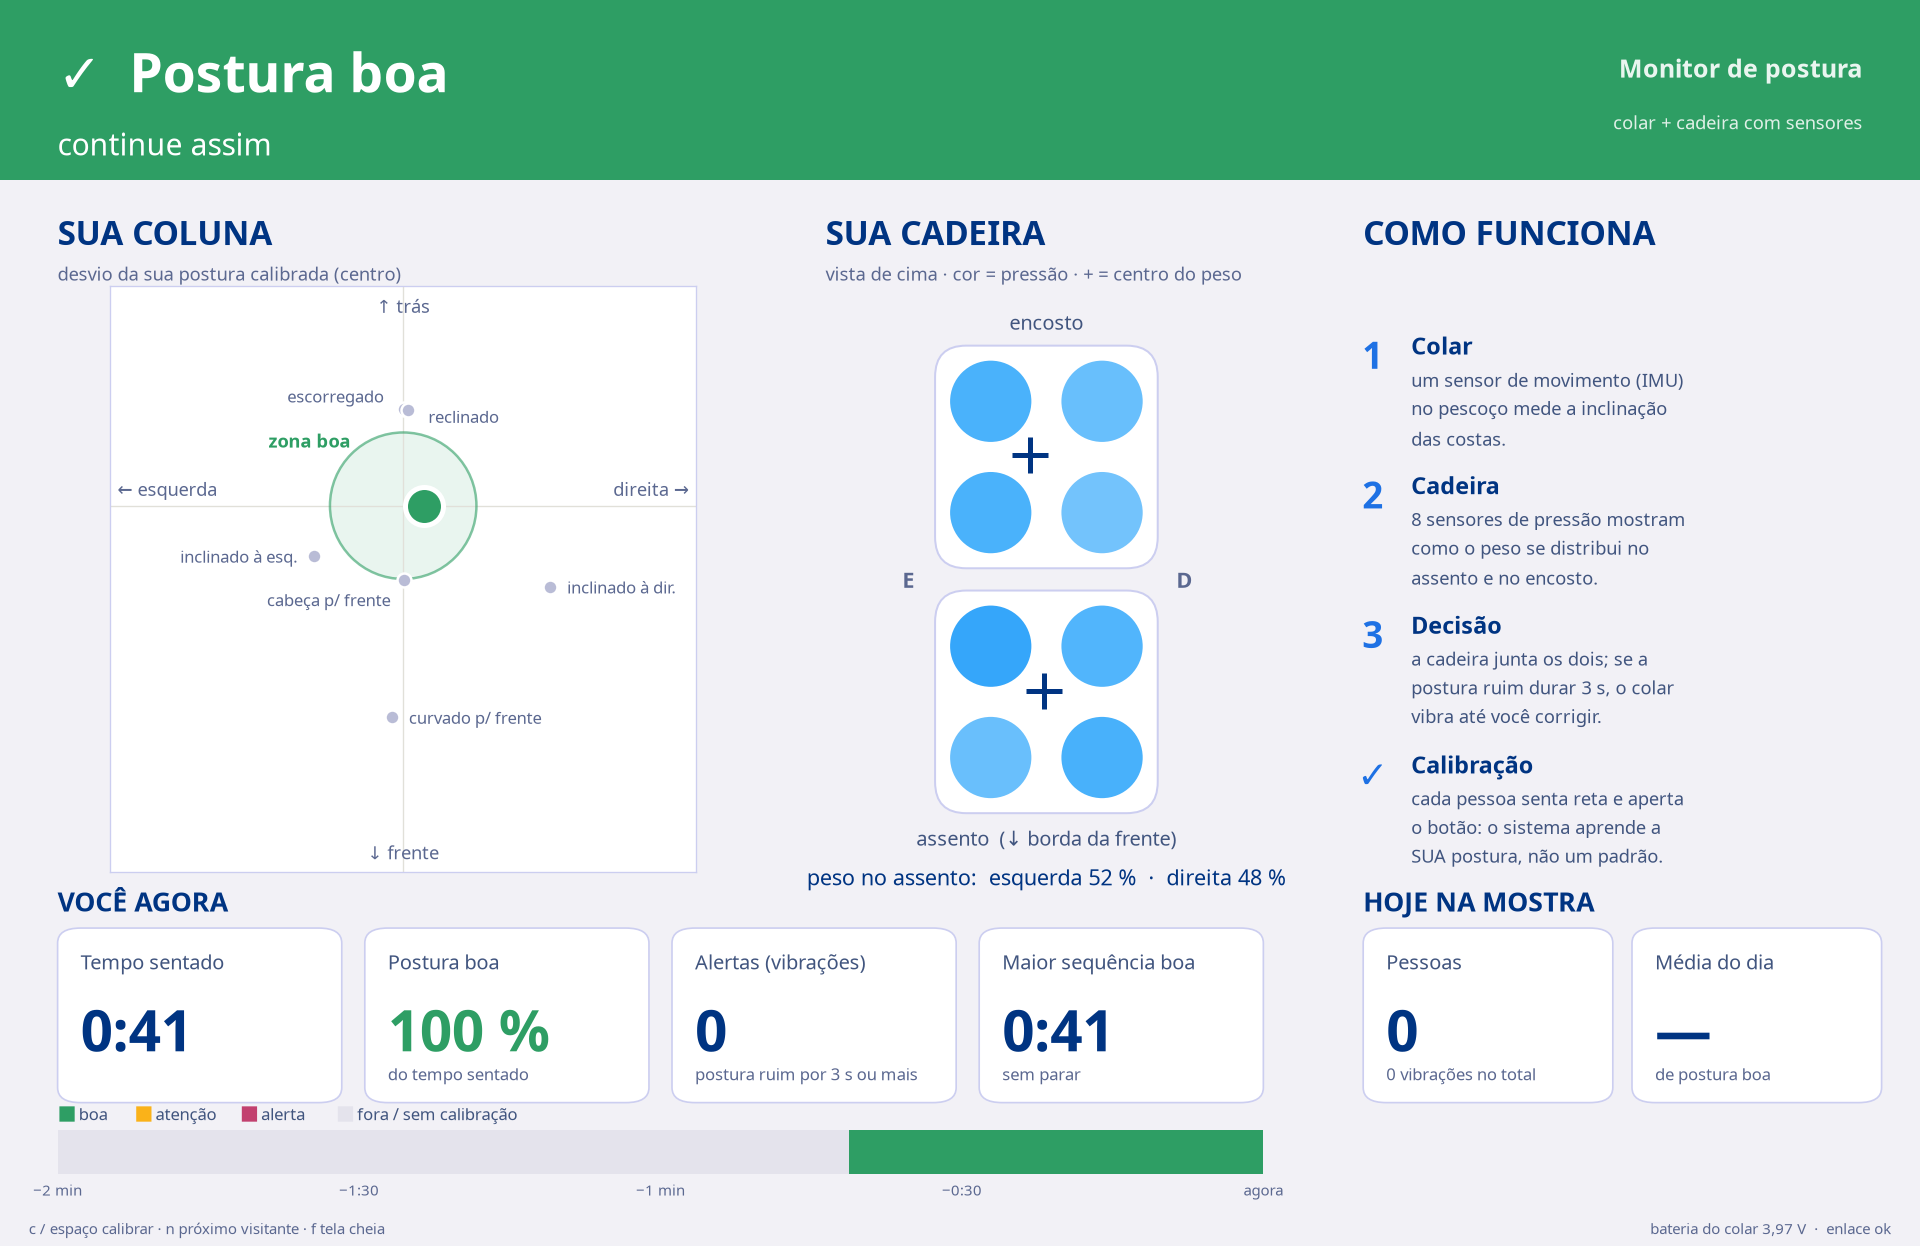
\includegraphics[width=\linewidth]{met-dashboard-boa.png}
  \fonte{Elaborado pelo autor (2026), captura disponível em \texttt{docs/stand}}
\end{figure}

O modo padrão prioriza USB, passa ao BLE após desconexão ou 1\,s
sem dados USB válidos e retorna ao cabo quando os dados reaparecem.
Somente uma fonte alimenta a tela a cada instante; no modo automático,
usa-se o relógio monotônico do notebook para manter a continuidade da
visita. Em BLE, a calibração depende do botão físico. A interface
tolera intervalos de até 2\,s para sua contabilização visual e
aguarda 5\,s de silêncio BLE para mostrar desconexão. Essa
continuidade estimada não recupera amostras perdidas. O modo
\texttt{--replay} reproduz CSVs sem hardware e mantém os contadores
da reprodução separados do dia real.

\subsubsection{Toolchain e testes automatizados}

Os programas embarcados são compilados com \texttt{arduino-cli},
core \texttt{Seeeduino:nrf52} versão 1.1.13 e alvo
\texttt{Seeeduino:nrf52:xiaonRF52840Sense}. A biblioteca local é
incluída por \texttt{--libraries firmware/libraries};
\texttt{Adafruit\_TinyUSB} acompanha o core. Para a bancada FSR
histórica utilizou-se o alvo \texttt{arduino:avr:uno}. As placas são
selecionadas para gravação por número de série USB, evitando depender
da numeração variável das portas.

A verificação automatizada tem três níveis. Primeiro, testes C++
exercitam protocolo, sequência, validade, portões temporais, bateria,
leitor inercial e formatação serial. Segundo, os próprios programas
\texttt{body.ino} e \texttt{chair.ino} são compilados no computador
com substitutos de rádio, USB e IMU; \texttt{test\_system} executa
ambos sobre um enlace simulado. São exercitados perda de enlace,
reinicialização, duplicatas, host USB que deixa de ler e falhas
retornadas pelo barramento. Terceiro, testes Python verificam
carregadores, análise, leitores de transporte e sessões do dashboard.

O teste C++ \texttt{test\_fusion} compara motivo e alerta, amostra a
amostra, com trechos reais cujo resultado esperado foi gerado por
\texttt{analysis/fusion.py}. As bases e o estado inicial do portão
acompanham os trechos em \texttt{fusion\_cases.txt}. Os testes Python
também verificam a equivalência entre replay sequencial e vetorizado
e a leitura de saídas do sistema simulado. Essa comparação confere a
transposição da regra para C++; não constitui validação independente
dos limiares nos usuários.

O \texttt{Makefile} de \texttt{firmware/test} usa C++11, avisos como
erros e sanitizadores de endereço e comportamento indefinido. Há um
teste adicional com \texttt{-Ofast}, opção do core que pode eliminar
verificações usuais de \texttt{NaN}; por isso o protocolo inspeciona a
representação IEEE-754 dos números. Os comandos de reprodução são
\texttt{make -C firmware/test} e, para a suíte Python,
\texttt{QT\_QPA\_PLATFORM=offscreen} seguido de
\texttt{.venv/bin/python -m unittest discover -s analysis}.
Os substitutos em host não reproduzem um barramento físico travado
nem todos os aspectos temporais do microcontrolador, devendo ser
complementados pela observação em hardware.

\subsection{Procedimentos experimentais e avaliação}
\label{sec:met-experimentos}

\subsubsection{Caracterização em bancada: Campanhas A e B}

Na etapa parcial, realizada em junho de 2026, os canais foram
caracterizados separadamente. A Campanha A empregou um participante
com o XIAO sem o colar/invólucro final, fixado abaixo do pescoço e
conectado por USB. Registraram-se posturas mantidas por aproximadamente
10\,s, com movimentos rotulados e excluídos da análise. Retiradas e
recolocações do sensor, seguidas de calibração, permitiram avaliar a
dependência da referência em relação à montagem. Os scripts de
validação e visualização estão em \texttt{analysis/archive}.

A codificação dessa campanha foi distinta da integrada: 0 indicava
ereto; 1, curvar para a frente; 2 e 3, inclinações laterais; 4,
cabeça baixa; 5, recostar com quadril à frente; e 9, transição.
Não se equiparou automaticamente essa última postura à reclinação
apoiada definida no protocolo final. A série registrada utilizou
posturas pronunciadas, não representando uso natural contínuo.

A Campanha B utilizou Arduino Uno, FSR402 e divisor com resistor
medido de 2833\,\ohm, alimentado a 5\,V, com ADC de dez bits.
Foram caracterizadas três peças físicas, com carga aplicada por
elemento rígido centralizado sobre o sensor e lida em balança.
O protocolo de precisão incluiu níveis próximos de 50, 100, 200, 400,
800, 1200, 1600 e 2000\,g, em subida e descida, retenção de cerca
de 5\,s por nível e ensaio de deriva sob massa constante próxima
de 1\,kg, planejado por 10\,min.

O tratamento recuperou resistência a partir do divisor, reuniu níveis
com pequenas oscilações da carga digitada e comparou medianas,
trajetórias de carga/descarga, condutância e modelos de resposta.
As capturas passaram pelo validador \texttt{validate\_fsr.py}.
Esses ensaios caracterizam sensores e montagem de bancada, não
calibram força na espuma da cadeira integrada. Os resultados de
ambas as campanhas são apresentados na Seção~\ref{sec:resultados}.

\subsubsection{Capturas integradas de 21 de outubro de 2026}

O conjunto de desenvolvimento contém nove arquivos de oito sujeitos,
com duas sessões de um mesmo participante mantidas sob a mesma
identidade. Os CSVs reúnem IMU e FSRs em um único relógio de recepção
da cadeira. O motor foi mantido mudo nas capturas de desenvolvimento,
para não orientar a autocorreção do participante nem introduzir
vibração na aquisição. Na ocasião, usou-se uma compilação com motor
silenciado; o mecanismo em execução \texttt{--motor-muted}, descrito
anteriormente, foi acrescentado depois e é o procedimento atual.
Não se atribuem retroativamente colunas da versão 5 aos logs de
21/10, identificados com protocolo 4.

A Tabela~\ref{tab:met-posturas} apresenta a codificação integrada.
O operador marca 0 antes de qualquer movimento e só seleciona a
postura após sua estabilização. As tags persistem até a próxima
tecla; descrevem a instrução dada ao participante e não uma medida
anatômica independente.

\begin{table}[H]
  \centering
  \begin{singlespace}
  \caption{Tags e posturas do protocolo do sistema completo.}
  \label{tab:met-posturas}
  \small
  \begin{tabularx}{\linewidth}{@{}c l X@{}}
    \toprule
    Tag & Postura & Instrução operacional \\
    \midrule
    0 & Transição & Movimento ou trecho não rotulado; excluído da pontuação. \\
    1 & Ereto & Sentar até o fundo, na postura de referência da calibração. \\
    2 & Curvado à frente & Curvar o tronco, retirando as costas do encosto. \\
    3 & Cabeça à frente & Manter o tronco apoiado e projetar cabeça/pescoço à frente. \\
    4 & Escorregado & Deslocar o quadril à frente, mantendo apenas as escápulas no encosto. \\
    5 & Inclinado à esquerda & Inclinar o tronco para a esquerda, apoiado no braço. \\
    6 & Inclinado à direita & Repetir a inclinação para a direita. \\
    7 & Reclinado & Apoiar o encosto inteiro, conservando o quadril atrás; aceitável. \\
    8 & Perna E sobre D & Cruzar a esquerda sobre a direita, com tronco ereto. \\
    9 & Perna D sobre E & Cruzar a direita sobre a esquerda, com tronco ereto. \\
    \bottomrule
  \end{tabularx}
  \end{singlespace}
  \fonte{Elaborado pelo autor (2026), a partir de \texttt{docs/protocolo-captura.md}}
\end{table}

O protocolo curto prevê aproximadamente 15\,s por postura e
10\,s de ereto entre posturas, duas passadas em ordem embaralhada,
série sutil e recolocação com nova calibração. Voltar o quadril ao
fundo depois de escorregar é uma instrução explícita para evitar
posturas combinadas. A ordem embaralhada busca separar efeitos de
postura dos efeitos de tempo, acomodação e deriva.

Entretanto, o registro de execução não sustenta que todos completaram
esse roteiro. As primeiras sessões foram séries marcadas em ordem
fixa; algumas tiveram uma passada, outras duas e recalibrações.
Somente as sessões de Gustavo e Rafael utilizaram a primeira passada
das folhas embaralhadas P1 e P2, respectivamente, com omissões
registradas na segunda. Por isso, a avaliação usa os segmentos
efetivamente disponíveis, sem supor um desenho balanceado, séries
sutis completas ou recolocações sistemáticas para os oito sujeitos.

Antes da análise, tomou-se o mapa corrigido para a perspectiva de
quem senta: os cabeçalhos de 21/10 haviam sido mapeados de frente
para a cadeira e tiveram esquerda/direita espelhadas, com nota de
proveniência. O registro também documenta correções pontuais de tags
e a separação de uma sessão anexada por engano a outro arquivo.
Preservaram-se as observações de deriva e de posturas mistas para
interpretar os limites do conjunto. Não se aplicou estatística
inferencial aos oito sujeitos.

\subsubsection{Reconstrução das calibrações e replay da decisão}

O carregador \texttt{captures.py} lê dados, eventos iniciados por
\texttt{\#}, mapa dos FSRs, tags e identificadores de calibração.
Quando a linha de base dos FSRs está gravada no evento de calibração,
ela é utilizada diretamente. Nos logs anteriores, reconstrói-se a
janela de 20 amostras: as 19 linhas anteriores a
\texttt{\# calibrated} e a primeira posterior, já com o novo
\texttt{calid}. Isso reproduz o instante em que a cadeira termina
a média e só então escreve a linha correspondente.

Verificam-se comprimento da janela, presença do evento inicial,
continuidade da sequência, sessão corporal e validade da IMU. Se
faltam linhas ou a janela é incoerente, a calibração é marcada como
não confiável e não participa da pontuação. Para uma calibração já
ativa antes do início do arquivo, sem evento disponível, usam-se as
primeiras 20 linhas daquele identificador como aproximação da base.
Esse recurso afeta os trechos iniciais não rotulados; uma base que
seria recusada pela regra final não habilita a avaliação.

O replay percorre cada sessão completa na ordem temporal original,
usando milissegundos inteiros da cadeira. Reaplica referências,
reinícios, pausas de captura e o portão temporal amostra a amostra.
Os trechos de transição continuam alimentando o estado da regra:
excluí-los do processamento alteraria a contagem dos 3\,s e a
histerese. Durante uma captura de referência, conserva-se o estado
do portão sem atualizá-lo, como no programa embarcado.

Um cuidado adicional distingue rejeição real e contrafactual. A
cadeira preserva a referência anterior se recusar uma nova captura.
Ao simular a recusa de uma calibração que o firmware antigo aceitou,
o replay não utiliza os desvios já registrados sob aquela referência
como se pertencessem à anterior; deixa esses trechos sem decisão
avaliável. Comparam-se as regras somente nas linhas calibradas com
base confiável e utilizável pela fusão final.

Para a pontuação, consideram-se as tags diferentes de 0 e descartam-se
os primeiros 2\,s após cada troca de tag. A expressão ``amostras
assentadas'' designa aqui esse recorte temporal estabilizado, não
uma seleção de acertos pelo estado previsto pelo detector. Cada
segmento é uma sequência contínua de uma tag, sob os critérios de
calibração válidos. O replay vetorizado acelera a busca, com
equivalência ao sequencial verificada pelos testes.

\subsubsection{Métrica, grade de candidatos e validação por sujeito}

As tags 2--6 integram o grupo com alerta esperado; 1, 7, 8 e 9
integram o grupo sem alerta esperado. Para cada segmento $s$, calcula-se
$a_s$, a fração das suas amostras estabilizadas avaliáveis em que o
alerta está ativo. A função de escolha é
\begin{equation}
 J=\frac{1}{2}\left[
 \frac{1}{|\mathcal{B}|}\sum_{s\in\mathcal{B}}a_s+
 \frac{1}{|\mathcal{A}|}\sum_{s\in\mathcal{A}}(1-a_s)
 \right],
 \label{eq:met-pontuacao}
\end{equation}
em que $\mathcal{B}$ reúne os segmentos ruins e $\mathcal{A}$, os
aceitáveis, incluindo pernas cruzadas. Trata-se da média entre
sensibilidade temporal média dos segmentos ruins e especificidade
temporal média dos aceitáveis. Cada segmento tem o mesmo peso dentro
do grupo; a função não é a fração global de amostras corretas nem a
proporção de segmentos em que ocorreu ao menos um disparo.

A busca em \texttt{fusion.py} compreende 2250 combinações:
\begin{itemize}[nosep]
  \item \texttt{ALERT\_DEG} em $\{8,9,10,11,12\}\degree{}$;
  \item \texttt{SLUMP\_FRAC} desabilitado ou em $\{0{,}2;\,0{,}3;\,0{,}4;\,0{,}5\}$;
  \item \texttt{RECLINE\_FRAC} em $\{0{,}5;\,0{,}6;\,0{,}7;\,0{,}8;\,0{,}9\}$
        ou desabilitado;
  \item \texttt{LEAN\_DEG} em $\{5,6,7,8\}\degree{}$ ou desabilitado;
  \item \texttt{LEAN\_LR} em $\{0{,}03;\,0{,}05;\,0{,}08\}$.
\end{itemize}
Mantêm-se \texttt{CLEAR\_DEG} igual a \texttt{ALERT\_DEG} menos $3\degree{}$
e permanência de 3\,s. A seleção utiliza a média da pontuação de
cada candidato e dos vizinhos a até um passo em cada eixo da grade,
para privilegiar regiões estáveis do espaço de parâmetros.

Aplicou-se validação deixando um sujeito de fora
(\emph{leave-one-subject-out}, LOSO): selecionam-se parâmetros com
sete sujeitos e avalia-se o oitavo, repetindo-se a separação por
identidade. As duas sessões de André permanecem juntas na mesma
dobra. Compara-se também a regra histórica somente inercial,
representada por \texttt{CURRENT}, com os termos FSR desligados.
Esse nome no script é histórico; a regra embarcada final é a fusão.
Uma seleção feita com todos os oito sujeitos é identificada como
ajuste no próprio conjunto, separadamente da avaliação LOSO.

Além da pontuação, os scripts produzem fração de tempo alertado por
postura, ocorrência de alerta por segmento e latência a partir da
marcação da tag. Essa latência não mede diretamente o atraso desde o
início físico do desvio: o participante pode ter assumido a postura
durante a transição, antes da tecla. A comparação entre replay e
coluna de alerta gravada também considera o arredondamento dos
ângulos a uma casa decimal. Resultados e divergências são reservados
à Seção~\ref{sec:resultados}.

\subsubsection{Validação em hardware em 22 de outubro de 2026}

A regra de fusão foi gravada nas duas placas e exercitada com motor
ativo. Foram registradas duas sessões, sendo uma de André, já
presente no desenvolvimento, e uma de Lucas, primeiro sujeito novo.
A sessão de André utilizou a revisão \texttt{c4ae8f2}, em sequência
guiada, com retornos ao ereto, assento vazio, recolocação e nova
calibração. A de Lucas utilizou \texttt{b3c29b1}, protocolo 5,
com execução parcial da folha P3: tags 1, 5, 4, 8, 1, 2 e 6,
seguidas de aproximadamente 10\,s de cadeira vazia. Não foram
executadas nessa sessão as tags 3, 7 e 9, a segunda passada, a série
sutil ou a recolocação.

O procedimento verificou aquisição integrada, decisão transmitida,
vibração e retorno após correção, conservando o CSV para inspeção.
Somente o participante novo permite uma observação adicional fora
do conjunto usado na seleção, ainda limitada às posturas realizadas.
A identificação da cadeira e os detalhes de montagem do
colar/invólucro não foram registrados nessas sessões.

Esses arquivos foram obtidos antes da alteração que retém a última
orientação sem vibração, descrita na Seção~\ref{sec:met-corpo}.
O histórico \texttt{5e82e20}, seguido de \texttt{6eaafbe}, documenta
a introdução dessa proteção e o limite final de 1{,}5\,s.
Assim, o ensaio de 22/10 avalia a implementação que estava gravada
na ocasião; não é tratado como novo ensaio de hardware da correção
posterior. Uma repetição computacional dos ângulos retidos deve ser
identificada como simulação, sem substituir uma nova captura.

\subsubsection{Demonstração na feira de ciências}

Em novembro de 2026, o sistema completo foi demonstrado informalmente
a dezenas de pessoas, com calibração individual, observação da tela
do \texttt{mostra.py} e retorno vibratório. O fluxo consistiu em
colocar o colar, sentar até o fundo, calibrar pelo botão e demonstrar
curvatura, inclinação lateral, escorregamento, reclinação apoiada e
pernas cruzadas. O encerramento da visita e a limpeza da referência
preparavam o sistema para a próxima pessoa.

Essa atividade avaliou a operação pública do conjunto, com sensores,
atuador, alimentação e interface. Não houve sessões rotuladas ou
registro de dados experimentais para estimar sensibilidade,
especificidade ou taxa de acerto. Os contadores de demonstração do
dashboard não foram adotados como base quantitativa do relatório.
A feira é, portanto, distinguida das capturas controladas e da
avaliação por replay.

% REFERENCIAS NOVAS:
% Nenhuma referência bibliográfica externa nova. Os parâmetros e os
% procedimentos foram extraídos dos fontes, protocolos e registros
% versionados do próprio projeto, identificados no texto.

\section{Resultados}
\label{sec:resultados}

Apresentam-se a caracterização dos sensores, a avaliação nas capturas
integradas e a validação com motor ativo. A feira de ciências é relatada
separadamente, sem resultados quantitativos. O desfecho principal é detectar
postura prejudicial por alerta ativo ou inativo; identificar a classe de
postura é uma informação complementar.

\subsection{Caracterização dos sensores em bancada}
\label{sec:res-bancada}

\subsubsection{Orientação do tronco e referência individual}

Na bancada do IMU, com um participante e sem o suporte final do colar, a
principal sobreposição ocorreu entre curvar o tronco e abaixar a cabeça:
distância entre centroides de aproximadamente $6{,}9\degree{}$, contra pelo
menos $21{,}7\degree{}$ nos demais pares. A
Figura~\ref{fig:res-imu-bancada} retoma a variação da referência entre
montagens. A sobreposição limita a classificação dessas duas
posturas prejudiciais, mas não impede, por si só, sua detecção binária.

\begin{figure}[H]
  \centering
  \caption{Mudança da referência de ereto entre remontagens do IMU na
  campanha de bancada.}
  \label{fig:res-imu-bancada}
  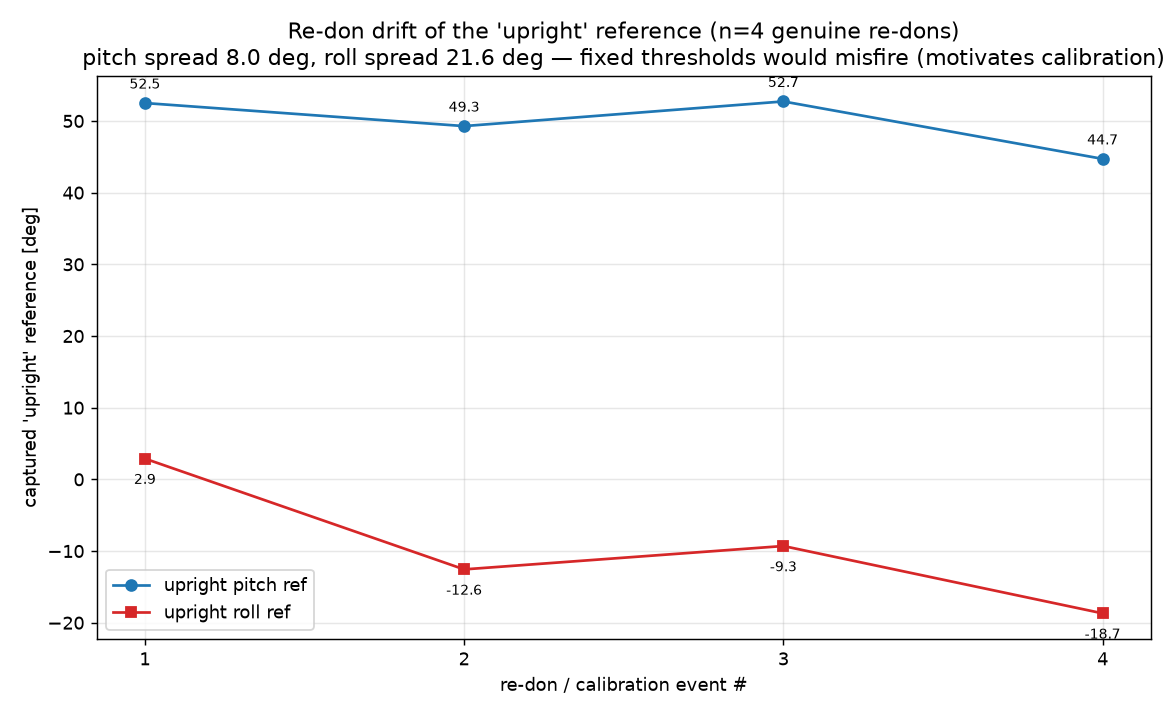
\includegraphics[width=0.80\linewidth]{04_redon_drift.png}
  \fonte{Elaborado pelo autor (2026)}
\end{figure}

Nas quatro épocas genuínas de retirada e recolocação, a referência de ereto
variou aproximadamente $8{,}0\degree{}$ em \textit{pitch} e $21{,}6\degree{}$
em \textit{roll}, valores comparáveis ou superiores ao desvio a detectar.
Isso sustenta a calibração individual em ereto. Trata-se de mudança da
montagem e da referência, não de deriva por integração do giroscópio: os
ângulos são estimados pelo acelerômetro.

O percentil 95 do módulo do desvio em ereto foi $6{,}4\degree{}$; o
percentil 5 agregado das posturas inadequadas foi $18{,}6\degree{}$.
O limiar inicial de $10\degree{}$ separou esses regimes, sem falso alarme e
com detecção de todas as posturas inadequadas nessa base. O resultado é
restrito a um participante e a movimentos pronunciados. As capturas
integradas mostram margens menores e falhas ausentes na bancada; a
orientação dos eixos na montagem final é indicada na
Seção~\ref{sec:res-capturas}.

\subsubsection{Resposta dos FSR402 e uso como pressão relativa}

A resistência do FSR1 caiu de aproximadamente 4134\,\ohm{} em
50\,g para 180\,\ohm{} no limite de aproximadamente 2\,kg da
balança. A maior redução ocorreu abaixo de 1{,}2\,kg. A curva se achatou,
mas continuou decrescendo: os valores de $160$--180\,\ohm{} nessa faixa
não representam um piso calibrado.

O ajuste por lei de potência apresentou $R^2$ de aproximadamente
$0{,}95$--$0{,}97$. A condutância, $G=1/R$, foi aproximadamente linear em
relação à carga, com $R^2$ próximo de $0{,}95$, superior ao ajuste linear da
própria resistência, próximo de $0{,}43$. A Figura~\ref{fig:res-fsr-modelo}
reproduz a comparação dos modelos e a estimativa de resolução da bancada.
A estimativa de cerca de 3\,\ohm{} por contagem em baixa resistência
corresponde ao ADC de 10 bits utilizado naquela etapa; não é a resolução do
circuito final, que lê contagens de 12 bits no XIAO.

\begin{figure}[H]
  \centering
  \caption{Modelos da resposta do FSR402 e resolução estimada na montagem de
  bancada da entrega parcial.}
  \label{fig:res-fsr-modelo}
  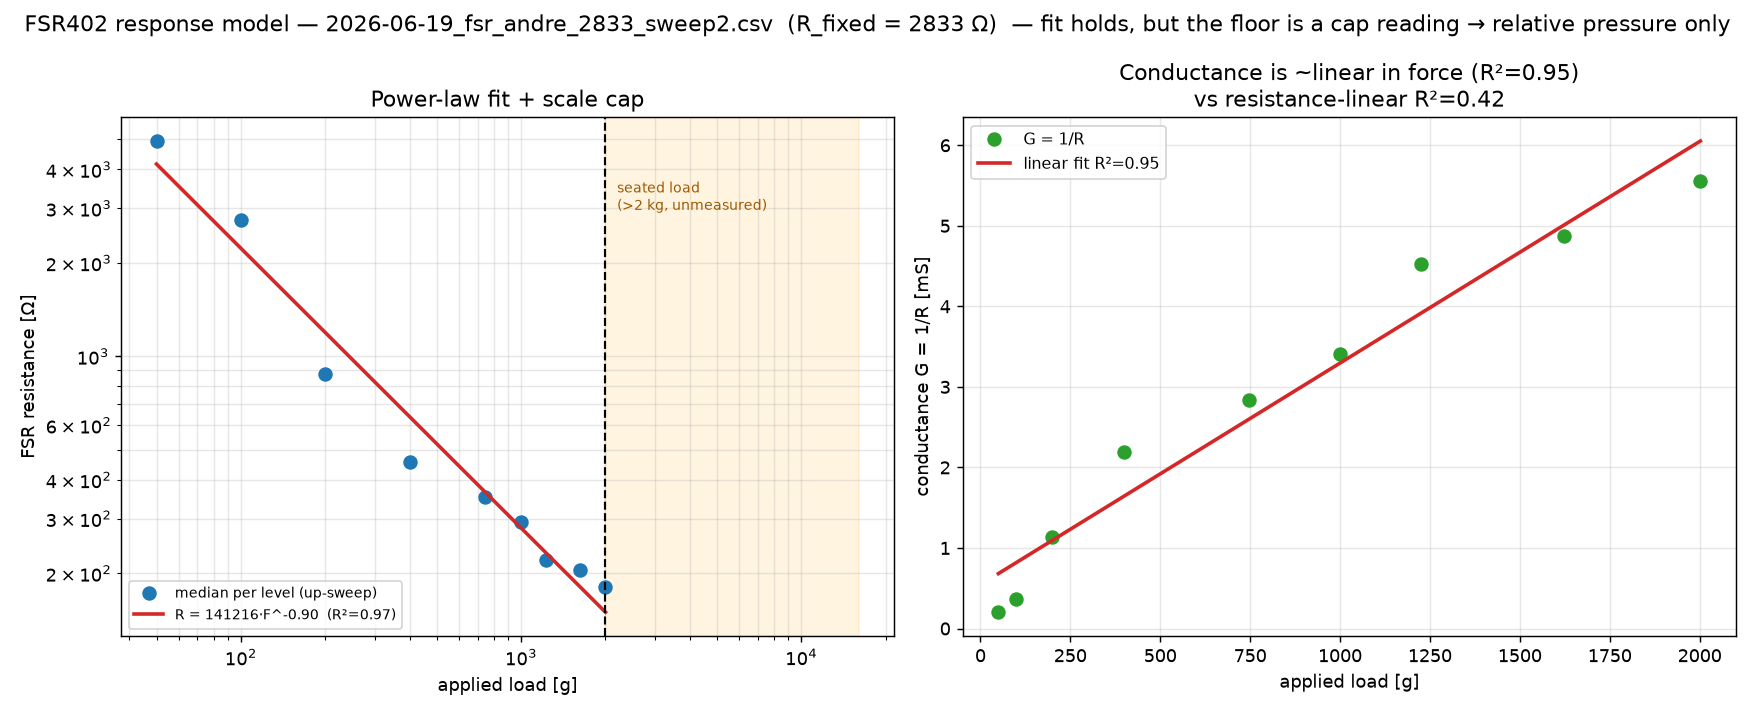
\includegraphics[width=0.96\linewidth]{fsr_model.png}
  \fonte{Elaborado pelo autor (2026)}
\end{figure}

A dependência do histórico de carga foi mais acentuada no regime leve. No
FSR2, a diferença entre descarga e carga passou de aproximadamente
$-76\,\%$ em 50\,g para $-6\,\%$ em 1\,kg. A histerese média
absoluta foi próxima de $52\,\%$ até 400\,g e de $6\,\%$ a partir de
1\,kg. Sob carga constante de 1\,kg, a resistência variou
$-7{,}4\,\%$ no FSR1 em cerca de 11 minutos e $-11{,}5\,\%$ no FSR2 em
cerca de 12 minutos. O \textit{creep} e a histerese impedem tratar cada
leitura como uma medida estável de força absoluta, mesmo que a direção da
resposta seja consistente.

A comparação entre três sensores, na Figura~\ref{fig:res-fsr-pecas}, mostrou
variações entre peças de aproximadamente $10$--$46\,\%$, conforme a carga.
Por exemplo, as medianas em 400\,g foram $453$, $514$ e 502\,\ohm{};
em 1\,kg, foram $290$, $267$ e 391\,\ohm{}. Variações maiores,
de três a onze vezes, apareceram em um transiente de acomodação do aplicador
rígido sobre um sensor. Esse transiente foi identificado como efeito da
montagem e excluído da comparação entre peças. Ele evidencia sensibilidade
à forma de aplicação da carga, mas não quantifica a variação de um FSR
instalado na espuma de uma cadeira sob um usuário.

\begin{figure}[H]
  \centering
  \caption{Variação entre três FSR402 nas varreduras de carga; os pontos
  associados à acomodação inadequada não representam dispersão entre peças.}
  \label{fig:res-fsr-pecas}
  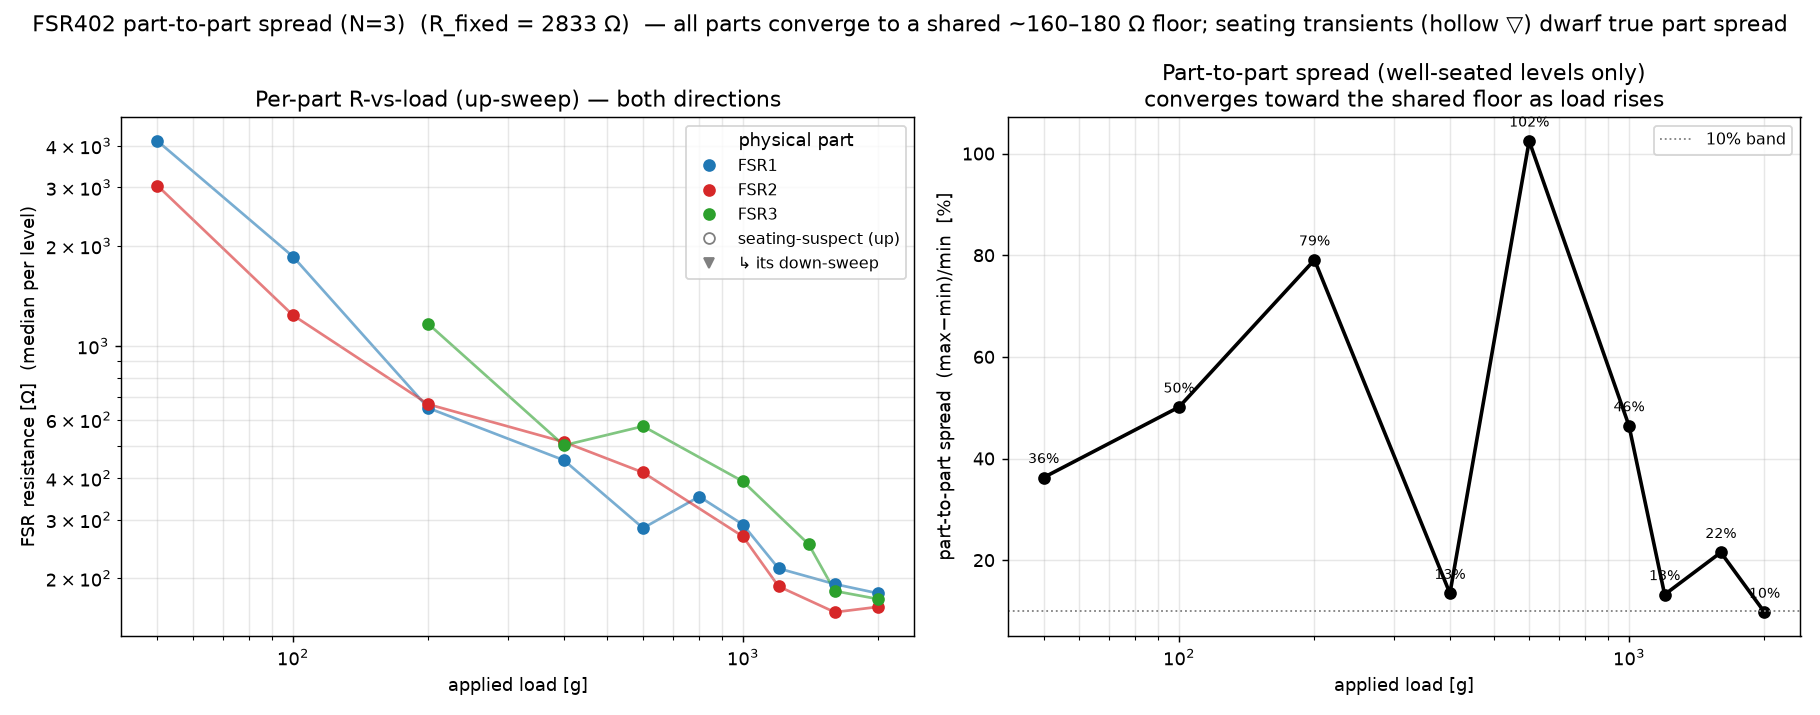
\includegraphics[width=0.94\linewidth]{fsr_parttopart.png}
  \fonte{Elaborado pelo autor (2026)}
\end{figure}

Esses resultados sustentam o uso dos FSRs como pressão relativa e contato.
A regra final utiliza somas de leituras cruas de grupos do assento e sua
relação com a linha de base individual, sem converter contagens em força.
A condutância auxilia a interpretação e a visualização; a decisão não exige
uma curva de força ajustada por sensor.

\subsection{Capturas do sistema completo em 21 de outubro de 2026}
\label{sec:res-capturas}

\subsubsection{Composição do conjunto de dados}

O conjunto integrado contém nove arquivos de oito participantes, com duas
sessões de André e uma de cada um dos demais participantes. Foram registradas
127773 amostras, em aproximadamente $106{,}5$ minutos de gravação. A
Tabela~\ref{tab:res-capturas} apresenta as durações por arquivo. O tempo com
presença estimada no assento foi de aproximadamente $103{,}5$ minutos;
transições, ajustes e intervalos sem etiqueta explicam por que esse tempo é
maior que o utilizado para pontuar as posturas.

\begin{table}[H]
  \centering
  \caption{Composição das nove capturas do sistema completo em 21/10/2026.}
  \label{tab:res-capturas}
  \begin{singlespace}
  \small
  \begin{tabularx}{\linewidth}{Xrrrr}
    \toprule
    Participante / sessão & Registro & Presença & Avaliado & Segmentos \\
                          & (min) & (min) & (min) & \\
    \midrule
    André / 1       & $5{,}62$  & $5{,}32$  & $2{,}71$  & 9 \\
    André / 2       & $23{,}87$ & $22{,}46$ & $10{,}92$ & 23 \\
    Felipe          & $8{,}36$  & $8{,}27$  & $3{,}35$  & 10 \\
    Gustavo         & $12{,}75$ & $12{,}63$ & $5{,}96$  & 16 \\
    Rafael          & $9{,}41$  & $9{,}12$  & $5{,}13$  & 11 \\
    Ryan            & $18{,}61$ & $18{,}40$ & $7{,}42$  & 18 \\
    Thiago Fita     & $13{,}07$ & $12{,}60$ & $7{,}68$  & 16 \\
    Thiago M.       & $7{,}25$  & $7{,}20$  & $3{,}87$  & 10 \\
    Vinicius        & $7{,}55$  & $7{,}53$  & $3{,}71$  & 10 \\
    \midrule
    Total           & $106{,}48$ & $103{,}54$ & $50{,}74$ & 123 \\
    \bottomrule
  \end{tabularx}
  \fonte{Elaborado pelo autor (2026)}
  \end{singlespace}
  \par\smallskip
  {\footnotesize Registro: diferença entre o último e o primeiro instante de
  cada arquivo. Presença: soma dos quatro FSRs do assento de pelo menos 2000
  contagens. Avaliado: amostras rotuladas, sob calibração válida, após excluir
  os primeiros 2\,s de cada segmento. Presença e tempo avaliado são estimados
  pelo número de amostras dividido por 20\,Hz; totais calculados antes do
  arredondamento.}
\end{table}

Foram aproveitados 123 segmentos, correspondentes a 3044{,}6\,s de
amostras estabilizadas. Desses segmentos, 62 representam posturas para as
quais se espera alerta, 39 representam ereto ou reclinado e 22 representam
pernas cruzadas, que não devem gerar alerta na versão avaliada. O número de
segmentos e o tempo por postura constam na Tabela~\ref{tab:res-posturas}.
Os códigos de postura desta campanha diferem dos utilizados na bancada de
junho; os números apresentados a seguir correspondem às etiquetas de outubro.

\begin{table}[H]
  \centering
  \caption{Distribuição dos segmentos e do tempo avaliado por postura.}
  \label{tab:res-posturas}
  \begin{singlespace}
  \begin{tabularx}{\linewidth}{cXrrc}
    \toprule
    Código & Postura & Segmentos & Tempo (s) & Alerta esperado \\
    \midrule
    1 & Ereto                 & 27 & $532{,}10$ & Não \\
    2 & Curvado à frente      & 13 & $301{,}80$ & Sim \\
    3 & Cabeça à frente       & 12 & $283{,}35$ & Sim \\
    4 & Escorregado           & 13 & $353{,}20$ & Sim \\
    5 & Inclinado à esquerda  & 12 & $326{,}95$ & Sim \\
    6 & Inclinado à direita   & 12 & $318{,}25$ & Sim \\
    7 & Reclinado             & 12 & $314{,}10$ & Não \\
    8 & Perna E sobre D       & 11 & $324{,}60$ & Não \\
    9 & Perna D sobre E       & 11 & $290{,}25$ & Não \\
    \midrule
      & Total                & 123 & $3044{,}60$ & \\
    \bottomrule
  \end{tabularx}
  \fonte{Elaborado pelo autor (2026)}
  \end{singlespace}
\end{table}

As sessões incluem ordens fixas, repetições, recalibrações e roteiros
abreviados ou embaralhados. Rafael não realizou as posturas 3 e 7.
As sessões de André foram mantidas juntas no LOSO. Os critérios estão na
Seção~\ref{sec:metodologia}. São dados exploratórios, sem estatística
inferencial nem ensaio de uso prolongado em trabalho de escritório.

\subsubsection{O que os canais inerciais distinguem}

No colar final, \texttt{dpitch} representa principalmente movimento lateral
(positivo à direita), e \texttt{droll}, sagital (positivo para trás).
A Figura~\ref{fig:res-imu-posturas} mostra as medianas por sujeito e postura,
reunindo as amostras estabilizadas das sessões de cada participante.

A curvatura pronunciada para frente produziu medianas de \texttt{droll}
entre aproximadamente $-19{,}4\degree{}$ e $-52{,}3\degree{}$, com
separação em relação ao ereto em todos os participantes. A postura de cabeça
à frente apresentou sinais menores e mais variáveis: em Gustavo, Thiago M.
e Vinicius, as medianas sagitais ficaram entre $-4{,}6\degree{}$ e
$-7{,}5\degree{}$. Esses valores explicam por que o bom resultado de bancada
não se transferiu integralmente para movimentos mais localizados no pescoço.

As inclinações laterais inverteram o sinal de \texttt{dpitch}, como esperado,
mas sua amplitude variou. Na inclinação à esquerda, Felipe apresentou mediana
de apenas $-6{,}2\degree{}$, enquanto Rafael chegou a $-27{,}1\degree{}$.
Na inclinação à direita de Vinicius, a mediana foi de aproximadamente
$10{,}5\degree{}$, próxima ao limiar. Já reclinar e escorregar para frente
produziram, em geral, desvios sagitais positivos. Esse sinal isolado não
informa se o quadril continua apoiado na parte traseira do assento, diferença
que passou a ser fornecida pelos FSRs.

\begin{figure}[H]
  \centering
  \caption{Medianas dos desvios do IMU por postura e participante nas capturas
  integradas; os valores numéricos preservam a leitura sem cores.}
  \label{fig:res-imu-posturas}
  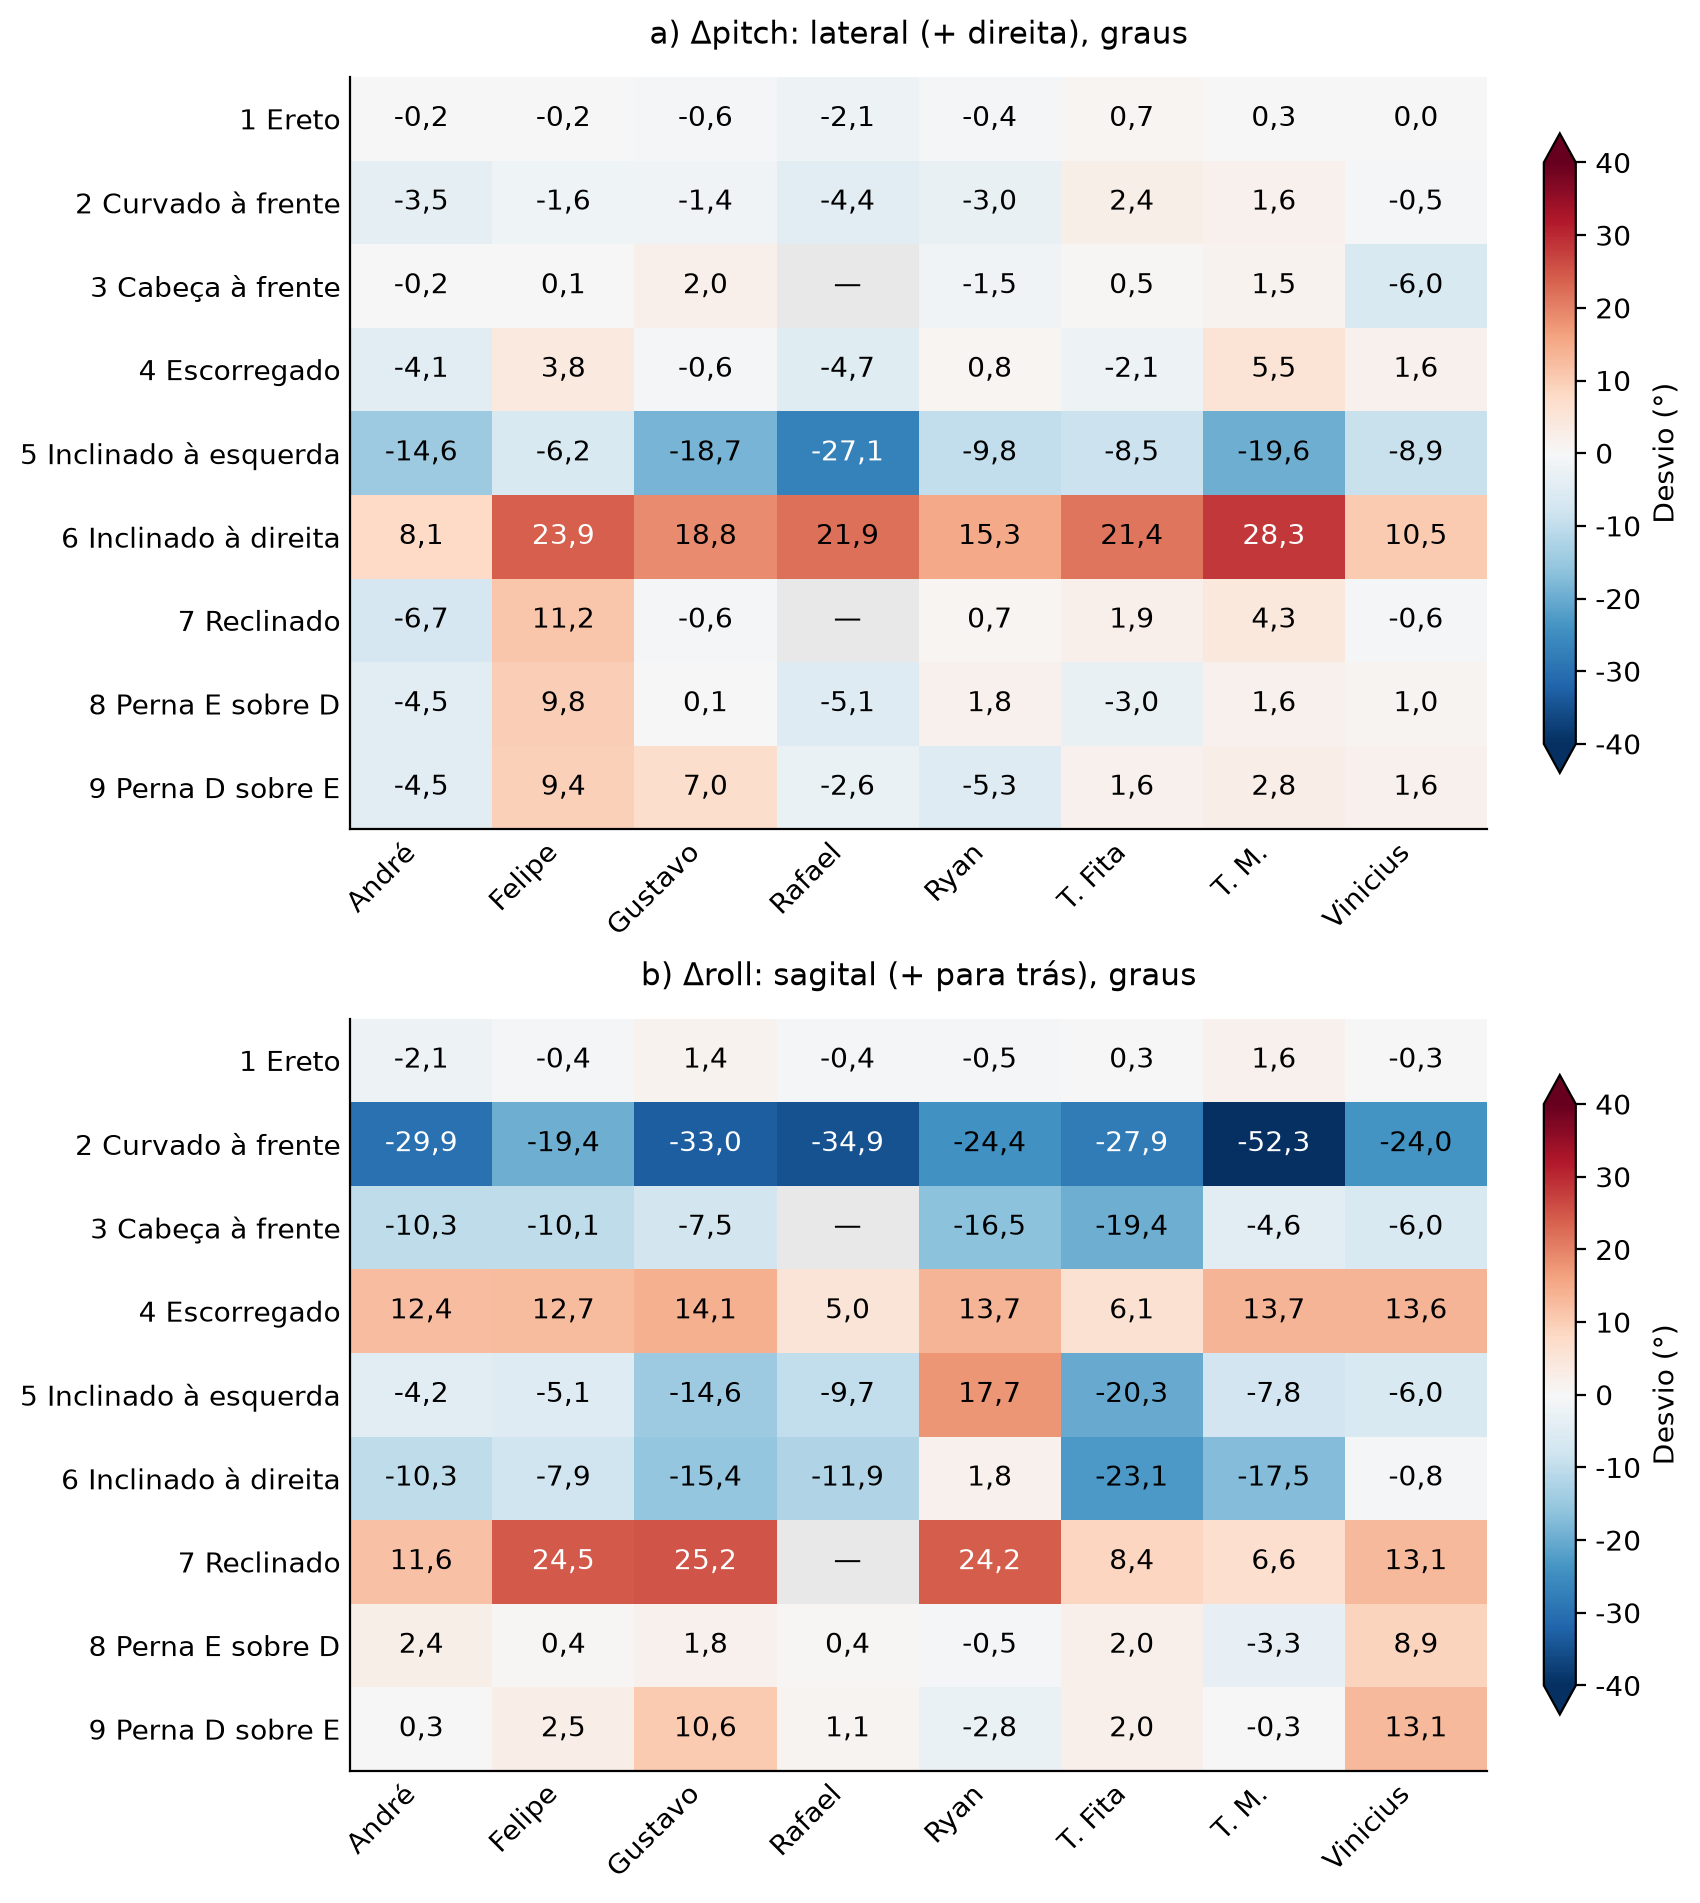
\includegraphics[width=\linewidth,height=0.76\textheight,keepaspectratio]{res_imu_posturas.png}
  \fonte{Elaborado pelo autor (2026)}
  \par\smallskip
  {\footnotesize E e D indicam esquerda e direita. T. Fita e T. M. são Thiago
  Fita e Thiago M. O traço indica postura não registrada, e não valor nulo.
  As escalas de cor são limitadas a $\pm40\degree{}$, mas as células mostram
  as medianas completas.}
\end{figure}

\subsubsection{Apoio traseiro e redistribuição lateral no assento}

A Figura~\ref{fig:res-assento-posturas} apresenta dois índices sem unidade:
a soma traseira dividida pela linha de base da calibração e a mudança do
índice esquerda/direita do assento em relação à mesma referência. A razão
traseira próxima de um indica apoio semelhante ao registrado em ereto; a
razão próxima de zero indica perda desse contato. No índice lateral, o sinal
positivo indica aumento relativo de leitura à esquerda. Essas grandezas
são razões de sinais elétricos, não frações calibradas do peso corporal.

Na postura escorregada, a mediana da razão traseira foi zero em 11 dos 13
segmentos. Os dois restantes apresentaram aproximadamente $0{,}23$ em uma
passagem de Thiago Fita e $0{,}49$ em Gustavo. Em contraste, no reclinado a
mediana agregada foi de aproximadamente $0{,}98$, com percentil 5 de
$0{,}65$. Portanto, os FSRs acrescentaram uma informação que o sentido da
inclinação do tronco não continha: a conservação ou perda de apoio do quadril.
No ereto, a razão traseira permaneceu entre $0{,}96$ e $1{,}09$ nos percentis
1 e 99 ao longo das sessões, cuja duração variou de cerca de 6 a 24 minutos.
Essa faixa ficou distante do limiar de escorregamento de $0{,}3$.

A redistribuição lateral foi menos uniforme que a perda de contato traseiro.
Em Felipe, a inclinação à esquerda combinou desvio inercial pequeno com
mediana de deslocamento lateral próxima de $+0{,}09$, suficiente para
confirmar a inclinação. Em Vinicius, a inclinação à direita produziu
aproximadamente $+0{,}04$, no sentido oposto ao esperado para essa postura,
impedindo a mesma confirmação. A mediana agregada também não descreve todas
as passagens: Ryan permaneceu escorregado durante uma inclinação à esquerda,
com perda de apoio traseiro, caracterizando uma postura mista.

Alguns canais inferiores do encosto permaneceram próximos de zero mesmo em
ereto, como em Rafael e Thiago M. Embora os oito FSRs sejam registrados,
a regra não utiliza razões individuais do encosto: seus índices decisivos
vêm dos grupos do assento. Não se demonstrou contribuição equivalente dos
oito pontos para o alerta.

\begin{figure}[H]
  \centering
  \caption{Medianas dos índices relativos do assento por postura e
  participante: apoio traseiro e deslocamento esquerda/direita.}
  \label{fig:res-assento-posturas}
  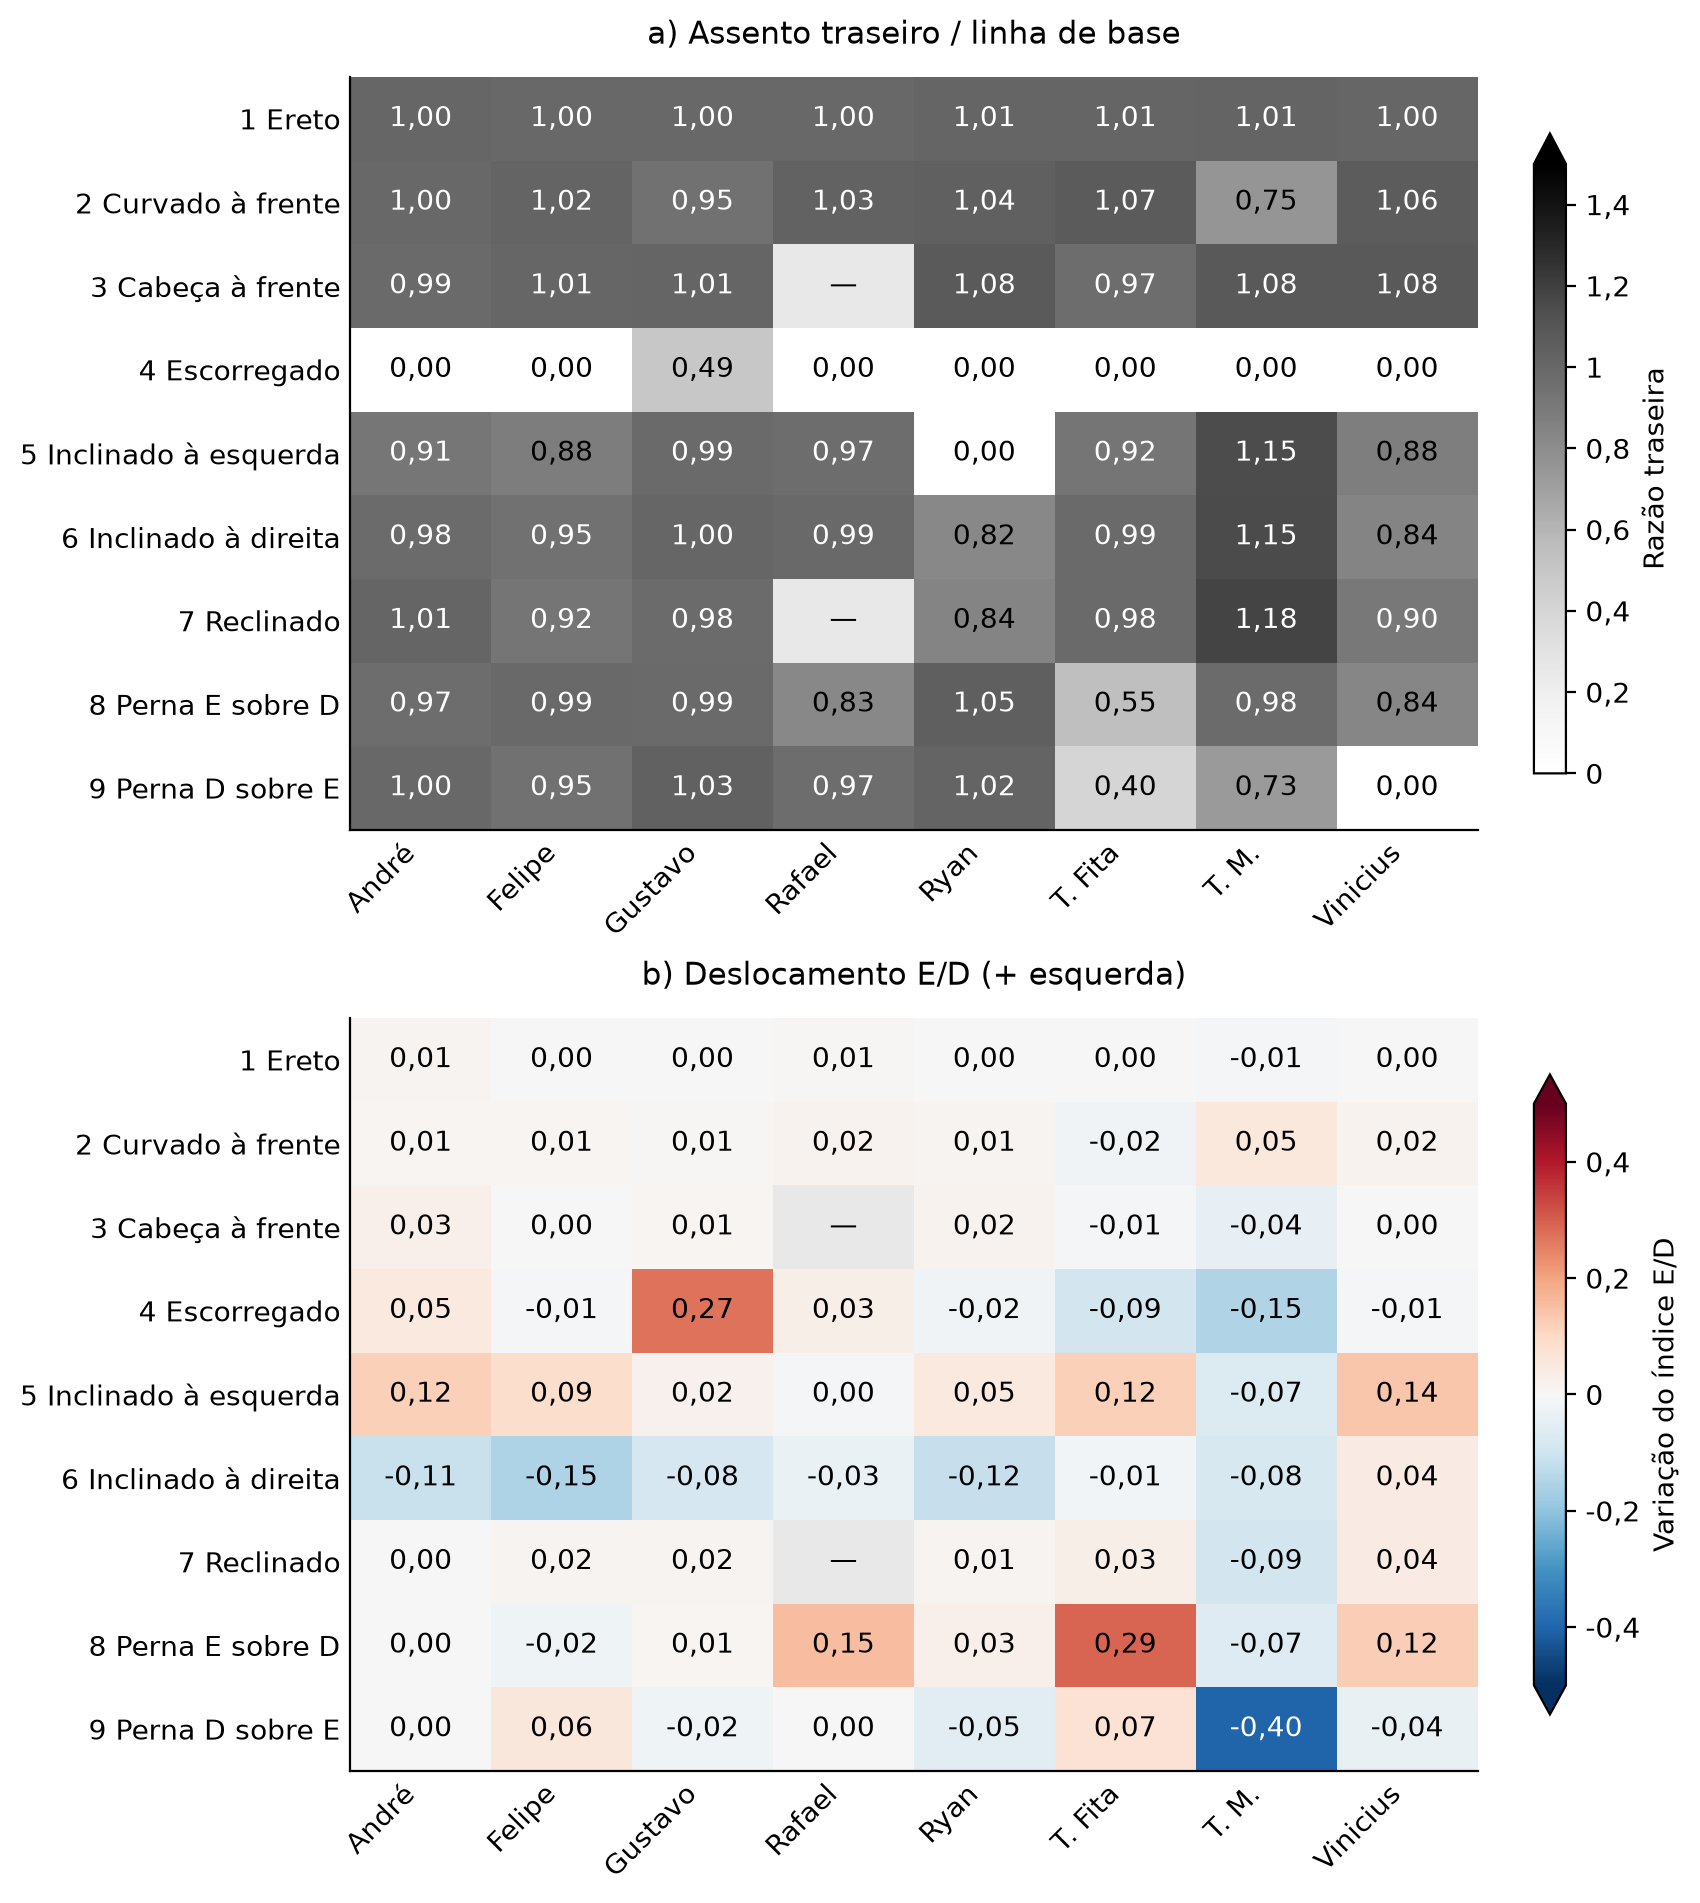
\includegraphics[width=\linewidth,height=0.76\textheight,keepaspectratio]{res_assento_posturas.png}
  \fonte{Elaborado pelo autor (2026)}
  \par\smallskip
  {\footnotesize Amostras estabilizadas sob calibração válida. O traço indica
  ausência de registro. Razão traseira igual a um e deslocamento lateral igual
  a zero correspondem à linha de base individual.}
\end{figure}

\subsection{Avaliação da regra de alerta}
\label{sec:res-alerta}

\subsubsection{Comparação global e avaliação LOSO}

A reprodução só-IMU concordou com o alerta original em
$99{,}74$--$100\,\%$ das amostras, conforme a sessão; diferenças pequenas
são compatíveis com ângulos arredondados próximos aos limiares.
Na Tabela~\ref{tab:res-comparacao}, a fusão final detectou 58/62 segmentos
prejudiciais, contra 55/62 da referência, elevando o tempo prejudicial
alertado de $84\,\%$ para $93\,\%$. O tempo ereto/reclinado alertado caiu de
$29\,\%$ para $2\,\%$. Percentuais de tempo ponderam as amostras;
a pontuação equilibra as frações por segmento conforme o protocolo.

\begin{table}[H]
  \centering
  \caption{Desempenho de detecção da referência só-IMU e da fusão nas capturas
  de 21/10/2026.}
  \label{tab:res-comparacao}
  \begin{singlespace}
  \small
  \begin{tabularx}{\linewidth}{Xccc}
    \toprule
    Indicador & Só-IMU & Fusão final & Fusão LOSO \\
    \midrule
    Segmentos prejudiciais com alerta & 55/62 & 58/62 & 58/62 \\
    Fração desses segmentos (\%) & 89 & 94 & 94 \\
    Tempo prejudicial com alerta (\%) & 84 & 93 & 92 \\
    Tempo ereto/reclinado com alerta (\%) & 29 & 2 & 3 \\
    Segmentos ereto/reclinado com alerta & 9/39 & 1/39 & 2/39 \\
    Tempo de pernas cruzadas com alerta (\%) & 10 & 11 & 28 \\
    Pontuação balanceada por segmento & $0{,}834$ & $0{,}935$ & $0{,}901$ \\
    \bottomrule
  \end{tabularx}
  \fonte{Elaborado pelo autor (2026)}
  \end{singlespace}
  \par\smallskip
  {\footnotesize Fusão final: parâmetros selecionados no conjunto completo.
  LOSO: resultado de cada sujeito com parâmetros selecionados sem seus dados.
  Segmento com alerta indica ao menos um alerta dentro do segmento, inclusive
  se iniciado antes da etiqueta. Percentuais arredondados ao inteiro.}
\end{table}

Em LOSO, a fusão conservou 58/62 segmentos detectados e $92\,\%$ do tempo
prejudicial alertado. O falso alarme foi de $3\,\%$ do tempo ereto/reclinado,
mas chegou a $28\,\%$ nas pernas cruzadas, avaliadas separadamente.
A pontuação caiu de $0{,}935$ para $0{,}901$, evidenciando a diferença entre
ajuste completo e transferência ao sujeito omitido. A referência só-IMU
não foi ajustada a essas capturas.

A execução de \texttt{analysis/fusion.py} reproduziu os totais da avaliação
documentada no repositório. A busca com todos os sujeitos retornou os
parâmetros finais: limiar angular de $10\degree{}$, limpeza abaixo de
$7\degree{}$, razão traseira de $0{,}3$ para escorregamento e de $0{,}7$
para admitir reclinação, além de confirmação lateral a partir de
$5\degree{}$ e deslocamento de $0{,}08$. Seis das oito dobras LOSO
selecionaram o limiar de $10\degree{}$; sete selecionaram cada um dos
limiares traseiros finais. Essa estabilidade parcial não elimina os casos
limítrofes discutidos a seguir.

\subsubsection{Desempenho por postura e participante}

A Tabela~\ref{tab:res-alerta-postura} mostra a fração do tempo com alerta por
postura. Valores altos são desejáveis nos códigos 2--6 e indesejáveis nos
códigos 1, 7, 8 e 9. Por isso, uma única taxa agregada de alerta não representa
a qualidade do sistema. A Figura~\ref{fig:res-alerta-sujeitos} detalha a fusão
final por participante e permite localizar os casos que limitam o resultado.

\begin{table}[H]
  \centering
  \caption{Percentual do tempo estabilizado com alerta por postura e regra.}
  \label{tab:res-alerta-postura}
  \begin{singlespace}
  \begin{tabularx}{\linewidth}{cXrrr}
    \toprule
    Código & Postura & Só-IMU & Fusão final & LOSO \\
    \midrule
    1 & Ereto                & 0 & 0 & 0 \\
    2 & Curvado à frente     & 100 & 100 & 100 \\
    3 & Cabeça à frente      & 70 & 70 & 70 \\
    4 & Escorregado          & 72 & 100 & 94 \\
    5 & Inclinado à esquerda & 94 & 100 & 100 \\
    6 & Inclinado à direita  & 87 & 93 & 94 \\
    7 & Reclinado            & 78 & 5 & 7 \\
    8 & Perna E sobre D      & 6 & 12 & 21 \\
    9 & Perna D sobre E      & 14 & 10 & 35 \\
    \bottomrule
  \end{tabularx}
  \fonte{Elaborado pelo autor (2026)}
  \end{singlespace}
\end{table}

\begin{figure}[H]
  \centering
  \caption{Tempo com alerta por participante e postura com a fusão final;
  células escuras indicam maior fração de alerta, não necessariamente acerto.}
  \label{fig:res-alerta-sujeitos}
  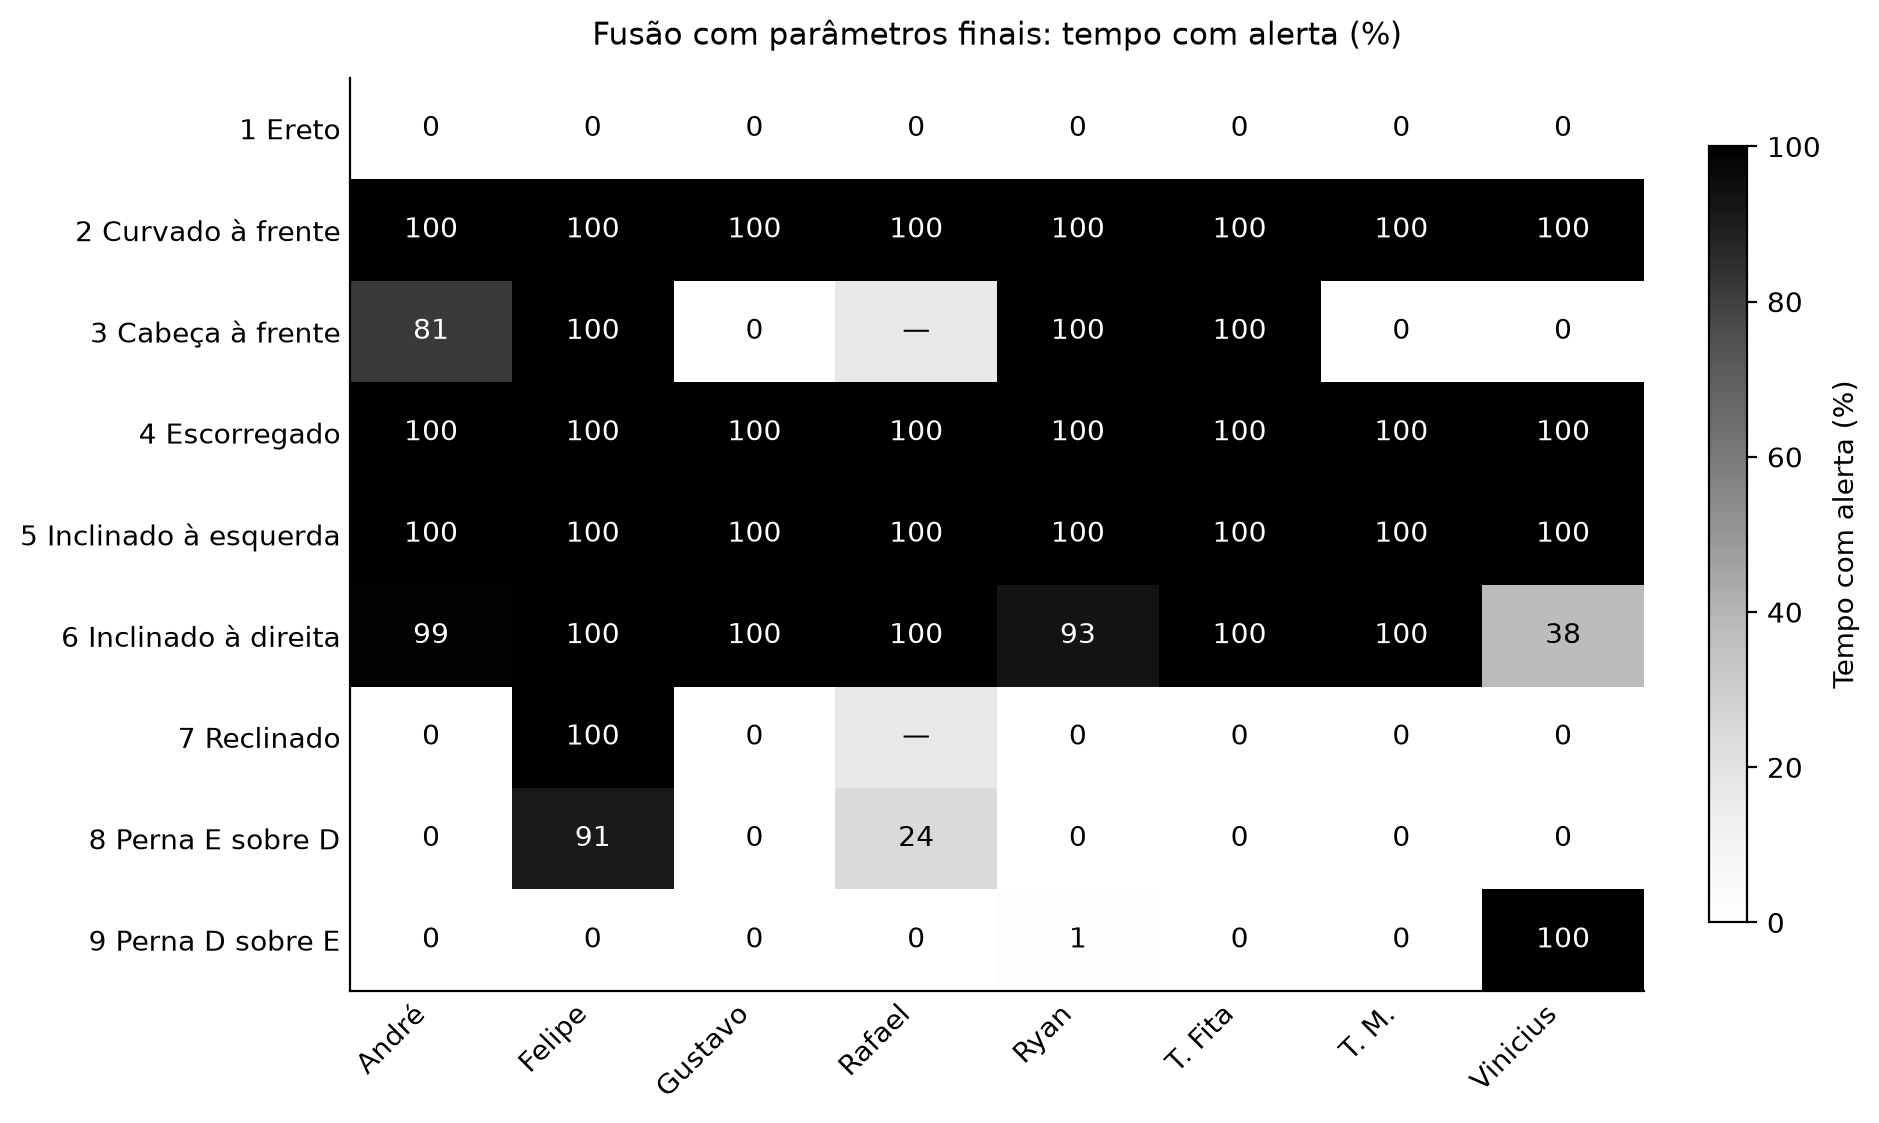
\includegraphics[width=\linewidth]{res_alerta_sujeitos.png}
  \fonte{Elaborado pelo autor (2026)}
  \par\smallskip
  {\footnotesize Percentuais ponderados pelo número de amostras estabilizadas.
  Espera-se alerta nas linhas 2--6 e ausência de alerta nas demais. Traço:
  postura não registrada.}
\end{figure}

A postura curvada para frente permaneceu alertada em todo o tempo avaliado
pelas três regras. O escorregamento passou de $72\,\%$ para $100\,\%$ com a
fusão final: a leitura do assento recuperou casos em que o tronco quase não
inclinou, como Rafael e parte das passagens de Thiago Fita. A inclinação à
esquerda passou de $94\,\%$ para $100\,\%$, incluindo o movimento de pequena
amplitude de Felipe. O reclinado apresentou a maior redução de falso alarme,
de $78\,\%$ para $5\,\%$ do tempo. O único segmento reclinado ainda alertado
com os parâmetros finais foi o de Felipe.

A pontuação de Vinicius passou de $0{,}67$ para $0{,}74$, mantida em LOSO;
a de Felipe passou de $0{,}68$ para $0{,}76$, caindo para $0{,}71$ em LOSO.
Ryan e Thiago Fita ficaram próximos de um com a fusão final. Portanto, o
resultado agregado não representa desempenho uniforme entre usuários.

\subsubsection{Contribuição de cada componente e cadeira vazia}

A ablação cumulativa, apresentada na Figura~\ref{fig:res-ablacao}, manteve os
parâmetros finais e ativou sucessivamente os componentes. A pontuação passou
de $0{,}834$ na regra só-IMU para $0{,}850$ com a detecção de escorregamento,
$0{,}922$ com o tratamento de reclinação e $0{,}935$ com a confirmação
lateral. O maior incremento correspondeu a deixar de penalizar a inclinação
para trás quando o apoio traseiro permanecia presente. Por ser uma ablação
cumulativa, os incrementos dependem da ordem de inclusão e não representam
contribuições estatisticamente independentes.

\begin{figure}[H]
  \centering
  \caption{Ablação cumulativa da regra de alerta com os parâmetros finais.}
  \label{fig:res-ablacao}
  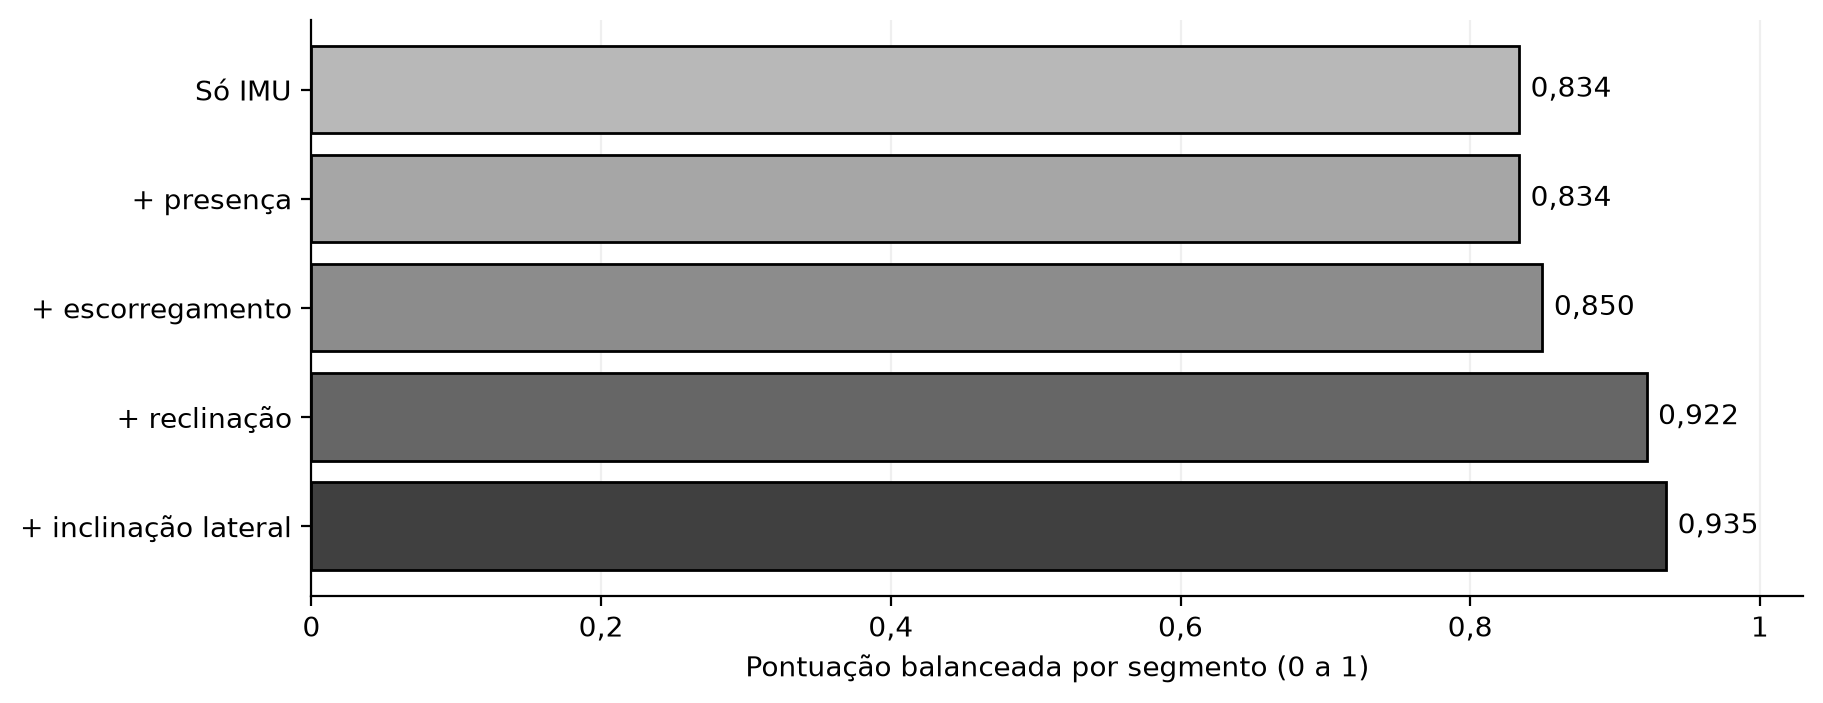
\includegraphics[width=0.98\linewidth]{res_ablacao.png}
  \fonte{Elaborado pelo autor (2026)}
\end{figure}

A supressão por presença não alterou a pontuação dos segmentos sentados,
mas evitou alertas nos intervalos de cadeira vazia. Com soma do assento
inferior a 2000 contagens, houve 176{,}30\,s de vazio: a referência alertou
em 70{,}85\,s e a fusão em 0\,s, aproximadamente os 176\,s e
71\,s documentados. Nesses intervalos, a pessoa podia estar em pé com o
colar; seu desvio inercial não indicava postura sentada inadequada.

\subsubsection{Falhas conhecidas, pernas cruzadas e limites temporais}

Na postura de cabeça à frente, Gustavo, Thiago M. e Vinicius não receberam
alerta. São três participantes entre os oito do conjunto, mas apenas sete
realizaram essa postura. A inclinação medida na região superior das costas
foi pequena e o contato com a cadeira permaneceu semelhante ao ereto. A fusão
não recuperou esses movimentos: o tempo alertado agregado continuou em
$70\,\%$. Reduzir o limiar frontal aproximaria a decisão do ereto de Rafael,
cujo percentil 5 de \texttt{droll} chegou a cerca de $-7{,}5\degree{}$.
Portanto, a falha não se resolve nos dados apenas supondo que os FSRs sempre
complementam um sinal inercial insuficiente.

Em Felipe, \texttt{dpitch} permaneceu próximo de $+10\degree{}$ após a
inclinação à direita. O reclinado alertou em $100\,\%$ do tempo e a perna
esquerda cruzada em $91\,\%$, sem mudança correspondente no assento.
A análise interpreta o padrão como deriva mecânica do colar ou da referência,
não como integração do giroscópio. A calibração inicial não assegura
estabilidade da fixação durante toda a sessão.

A inclinação à direita de Vinicius alertou em apenas $38\,\%$ do tempo:
o desvio ficou próximo do limiar e o assento deslocou no sentido oposto à
confirmação lateral. Também ocorreram posturas mistas: Vinicius escorregou
no código 9, gerando um alerta fisicamente justificável, mas contado como
falso alarme pela etiqueta; Ryan permaneceu escorregado no código 5,
continuando corretamente detectado. A classe dominante pode divergir da
etiqueta sem invalidar a detecção.

O cruzamento das pernas não apresentou padrão de pressão suficientemente
comum entre sujeitos. O módulo do deslocamento lateral excedeu $0{,}1$ em
apenas três dos oito participantes na postura 8; houve alterações por outros
índices na postura 9, mas sem direção consistente entre pessoas.
Com os parâmetros finais, os códigos 8 e 9 tiveram $12\,\%$ e $10\,\%$
do tempo alertado. Em Rafael, o código 8 apresentou $24\,\%$ de alerta por
confirmação lateral (Figura~\ref{fig:res-alerta-sujeitos}): a perna cruzada
deslocou a carga do assento enquanto o colar registrava inclinação lateral
próxima de $-5{,}7\degree{}$. A opção de não alertar
por pernas cruzadas corresponde ao escopo da regra avaliada, não a uma
conclusão clínica sobre essa posição.

O LOSO tornou algumas margens mais visíveis. Sem Thiago Fita, a escolha de
limiar traseiro $0{,}5$ passou a alertar sua postura 9, cuja razão traseira
foi de aproximadamente $0{,}40$. Sem Gustavo, o limiar de reclinação
$0{,}5$ reduziu a detecção do seu escorregamento a $23\,\%$ do tempo;
nesse caso a razão traseira era aproximadamente $0{,}49$. Sem André,
o limiar angular escolhido caiu para $8\degree{}$ e passou a gerar alertas
em trechos com pernas cruzadas e deslocamento lateral da referência.
Esses casos explicam a elevação de falso alarme nas pernas cruzadas em LOSO,
mesmo com manutenção do total de segmentos prejudiciais detectados.

Alerta em ao menos uma amostra não implica aviso sustentado. A histerese
pode transportar um alerta anterior se o desvio permanecer entre
$7\degree{}$ e $10\degree{}$. Latência zero desde a tecla também não
significa resposta instantânea: a pessoa frequentemente já havia cumprido
a espera de 3\,s durante a transição. A latência entre início físico do
movimento e vibração não foi medida.

\subsection{Validação em hardware em 22 de outubro de 2026}
\label{sec:res-hardware}

\subsubsection{Rodada guiada com participante já conhecido}

A primeira validação utilizou André, já presente no desenvolvimento, com
fusão nas placas e motor ativo (versão \texttt{c4ae8f2}). A rodada guiada,
com retenções de cerca de 16\,s, incluiu cadeira vazia, recolocação do
colar e recalibração. Os códigos 2--6 alertaram em $100\,\%$ do tempo
estabilizado; 1, 7, 8 e 9, em $0\,\%$. Os seis segmentos prejudiciais foram
detectados, incluindo duas ocorrências de escorregamento.

O participante percebeu a vibração e sua interrupção ao retornar ao ereto.
Não houve perda de pacotes nem indicação de falha do IMU. Verificou-se o
percurso entre sensores, decisão na cadeira, enlace e atuação corporal,
sem representar teste com pessoa nova ou medida de latência. Os detalhes de
ajuste do colar e da cadeira não foram registrados.

\subsubsection{Primeiro participante não utilizado no desenvolvimento}

Lucas Santos foi o primeiro participante sem dados nas capturas utilizadas
para escolher a regra. A sessão empregou a versão \texttt{b3c29b1}, com
protocolo de comunicação v5 e motor ativo. O roteiro foi parcial: ereto,
inclinado à esquerda, escorregado, perna esquerda sobre a direita, ereto,
curvado à frente e inclinado à direita, seguido de aproximadamente 10\,s
de cadeira vazia. Não foram realizadas as posturas 3, 7 e 9, a segunda
passagem, os movimentos sutis nem a recolocação do colar. Houve uma calibração,
sem perda de pacotes e sem indicação de falha do IMU.

A Tabela~\ref{tab:res-validacao} compara as duas sessões usando o alerta
registrado pelo firmware, e não uma previsão substituída pela reprodução.
Na sessão de Lucas, curvar para frente e escorregar produziram alerta em
$100\,\%$ do tempo estabilizado; ereto e cadeira vazia não produziram
alerta. Três problemas impediram a reprodução do resultado da rodada guiada:
instabilidade do alerta durante a vibração, perda da inclinação à direita
e alertas curtos com perna cruzada.

\begin{table}[H]
  \centering
  \caption{Tempo estabilizado com alerta registrado nas duas sessões de
  validação em hardware de 22/10/2026.}
  \label{tab:res-validacao}
  \begin{singlespace}
  \begin{tabularx}{\linewidth}{cXrr}
    \toprule
    Código & Postura & André (\%) & Lucas (\%) \\
    \midrule
    1 & Ereto                & 0 & 0 \\
    2 & Curvado à frente     & 100 & 100 \\
    3 & Cabeça à frente      & 100 & --- \\
    4 & Escorregado          & 100 & 100 \\
    5 & Inclinado à esquerda & 100 & $9{,}2$ \\
    6 & Inclinado à direita  & 100 & 0 \\
    7 & Reclinado            & 0 & --- \\
    8 & Perna E sobre D      & 0 & $2{,}9$ \\
    9 & Perna D sobre E      & 0 & --- \\
    \bottomrule
  \end{tabularx}
  \fonte{Elaborado pelo autor (2026)}
  \end{singlespace}
  \par\smallskip
  {\footnotesize Excluídos os primeiros 2\,s de cada segmento, como na
  avaliação anterior. Traço: postura não realizada. Os valores de Lucas
  para os códigos 5 e 8 são $11{,}6\,\%$ e $2{,}6\,\%$, respectivamente,
  quando se considera todo o intervalo rotulado, sem essa exclusão.}
\end{table}

A Figura~\ref{fig:res-validacao-lucas} mostra a perda de apoio traseiro no
escorregamento, detectado mesmo com desvio frequentemente abaixo de
$10\degree{}$, e o alerta sustentado na curvatura à frente. A inclinação
à direita não satisfez os critérios.

\begin{figure}[H]
  \centering
  \caption{Linha do tempo da sessão de Lucas: desvio registrado pela cadeira,
  razão traseira do assento, alerta registrado e etiqueta da postura.}
  \label{fig:res-validacao-lucas}
  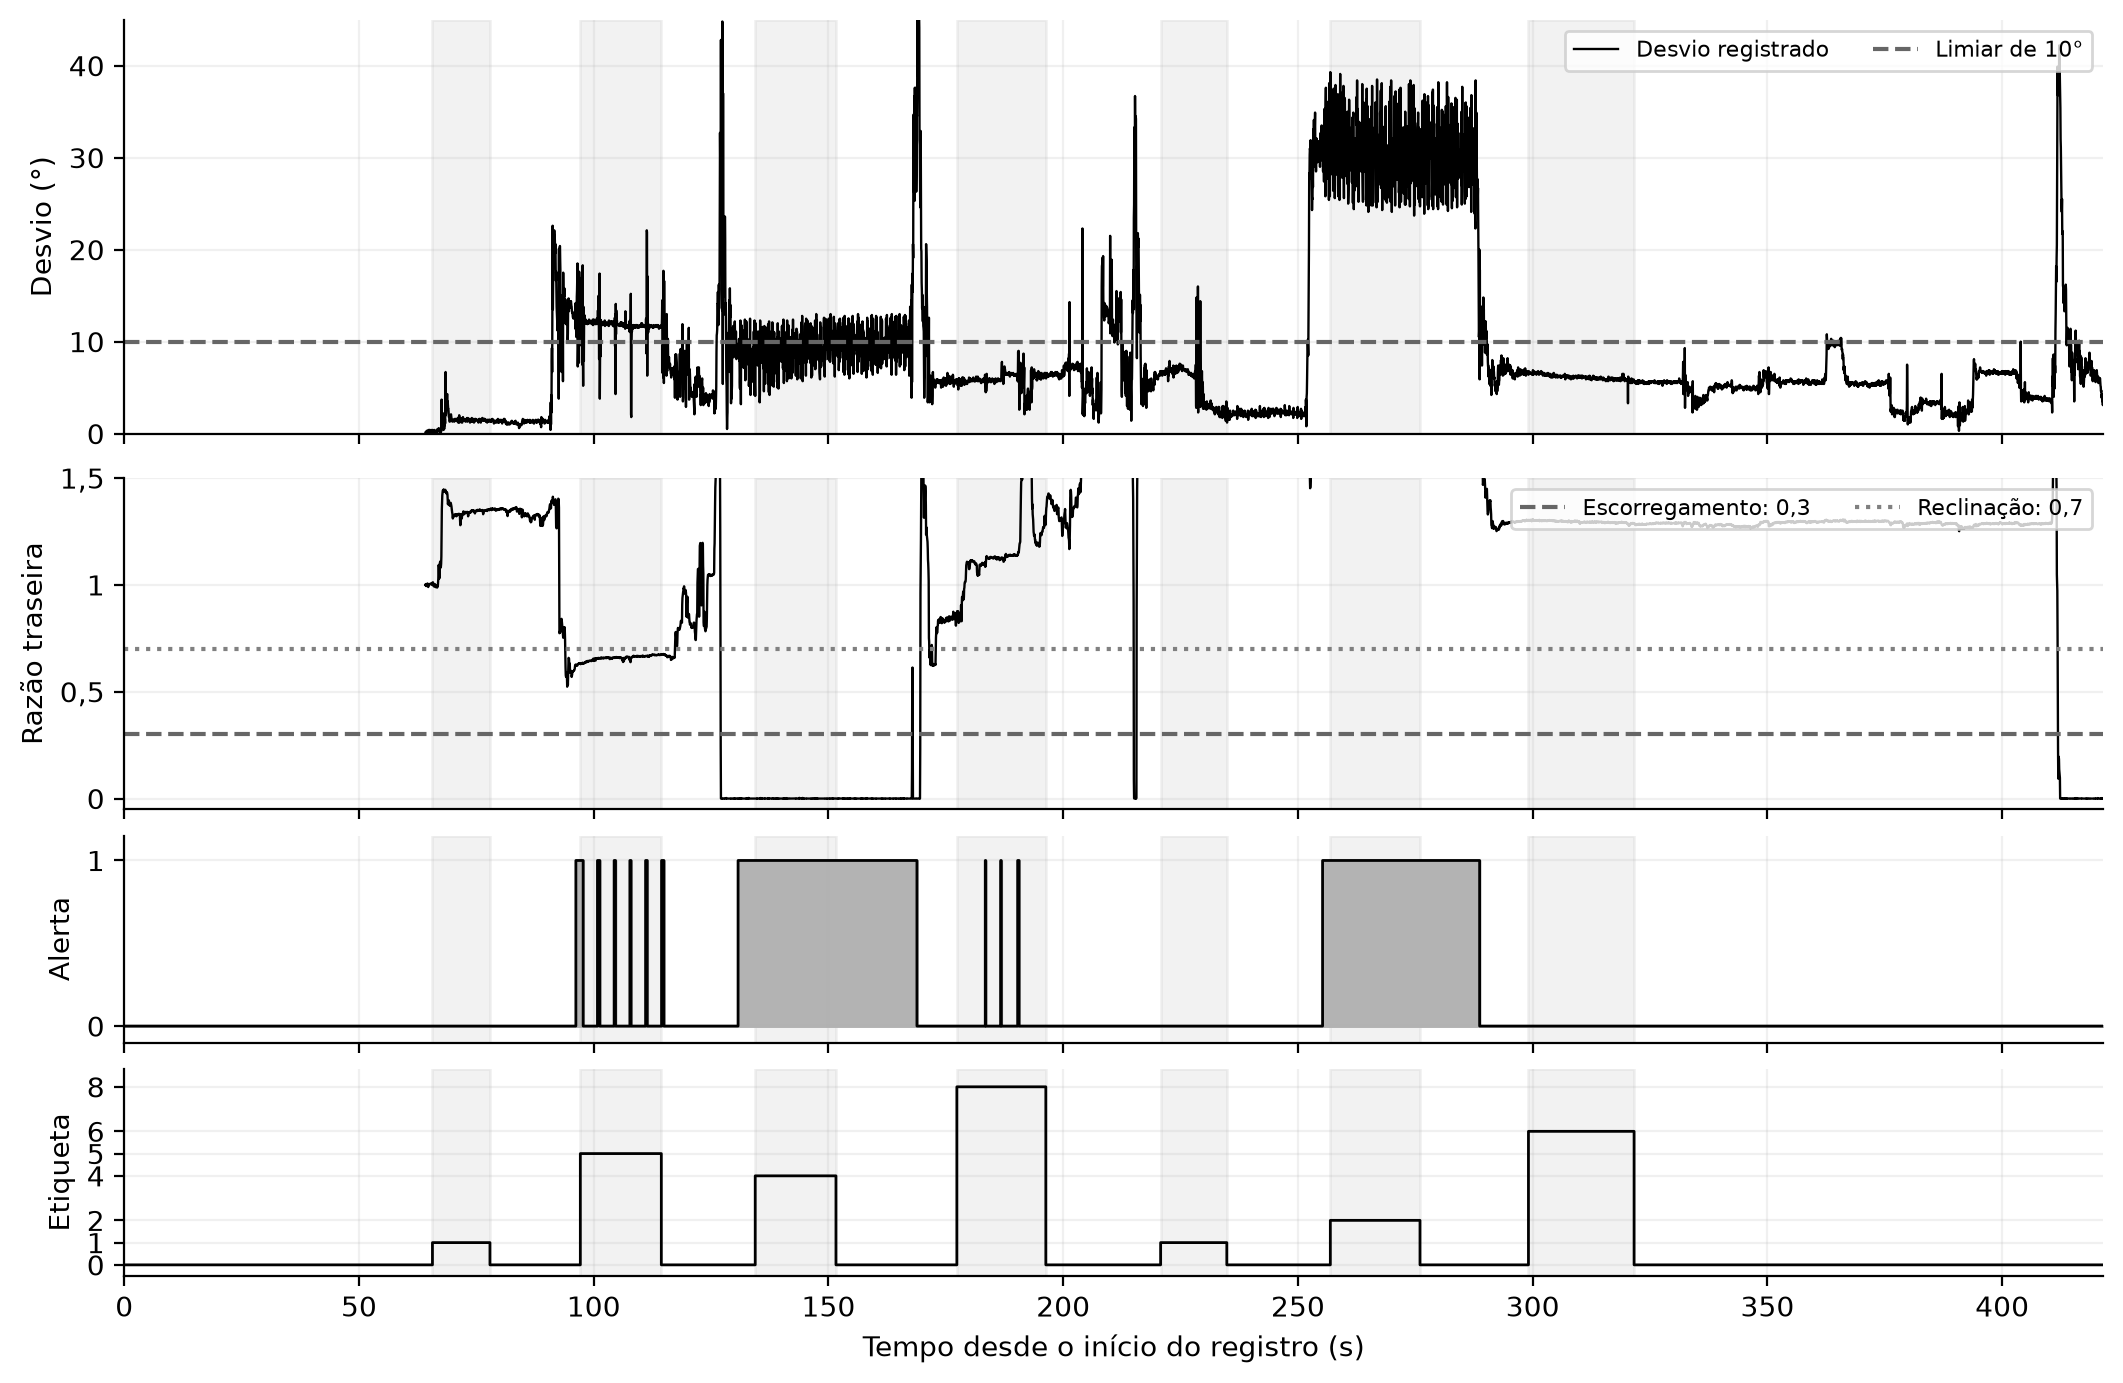
\includegraphics[width=\linewidth]{res_validacao_lucas.png}
  \fonte{Elaborado pelo autor (2026)}
  \par\smallskip
  {\footnotesize As faixas cinza indicam intervalos rotulados; etiqueta zero
  indica transição ou intervalo sem postura marcada. A leitura anterior à
  calibração não é mostrada nos dois primeiros painéis. Os eixos de desvio e
  razão traseira são limitados para favorecer a leitura das posturas mantidas;
  picos de movimento podem ultrapassar esses limites.}
\end{figure}

Na inclinação à esquerda, o desvio ficou próximo de $12\degree{}$ e a
condição de postura inadequada esteve presente entre os pulsos do motor.
Entretanto, o início da vibração provocou oscilações da ordem de
$\pm10\degree{}$ no IMU, com amostras abaixo do limiar de limpeza de
$7\degree{}$. Cada limpeza exigiu nova permanência de 3\,s para reativar
o alerta. A Figura~\ref{fig:res-motor-lucas} mostra as quedas abruptas do
desvio próximas aos pulsos reportados pelo corpo. O registro da análise
identificou seis reinícios desse tipo, produzindo avisos breves em vez de
uma sequência sustentada de vibração.

\begin{figure}[H]
  \centering
  \caption{Interferência da vibração na inclinação à esquerda de Lucas:
  oscilações do desvio, limiares e interrupções do alerta.}
  \label{fig:res-motor-lucas}
  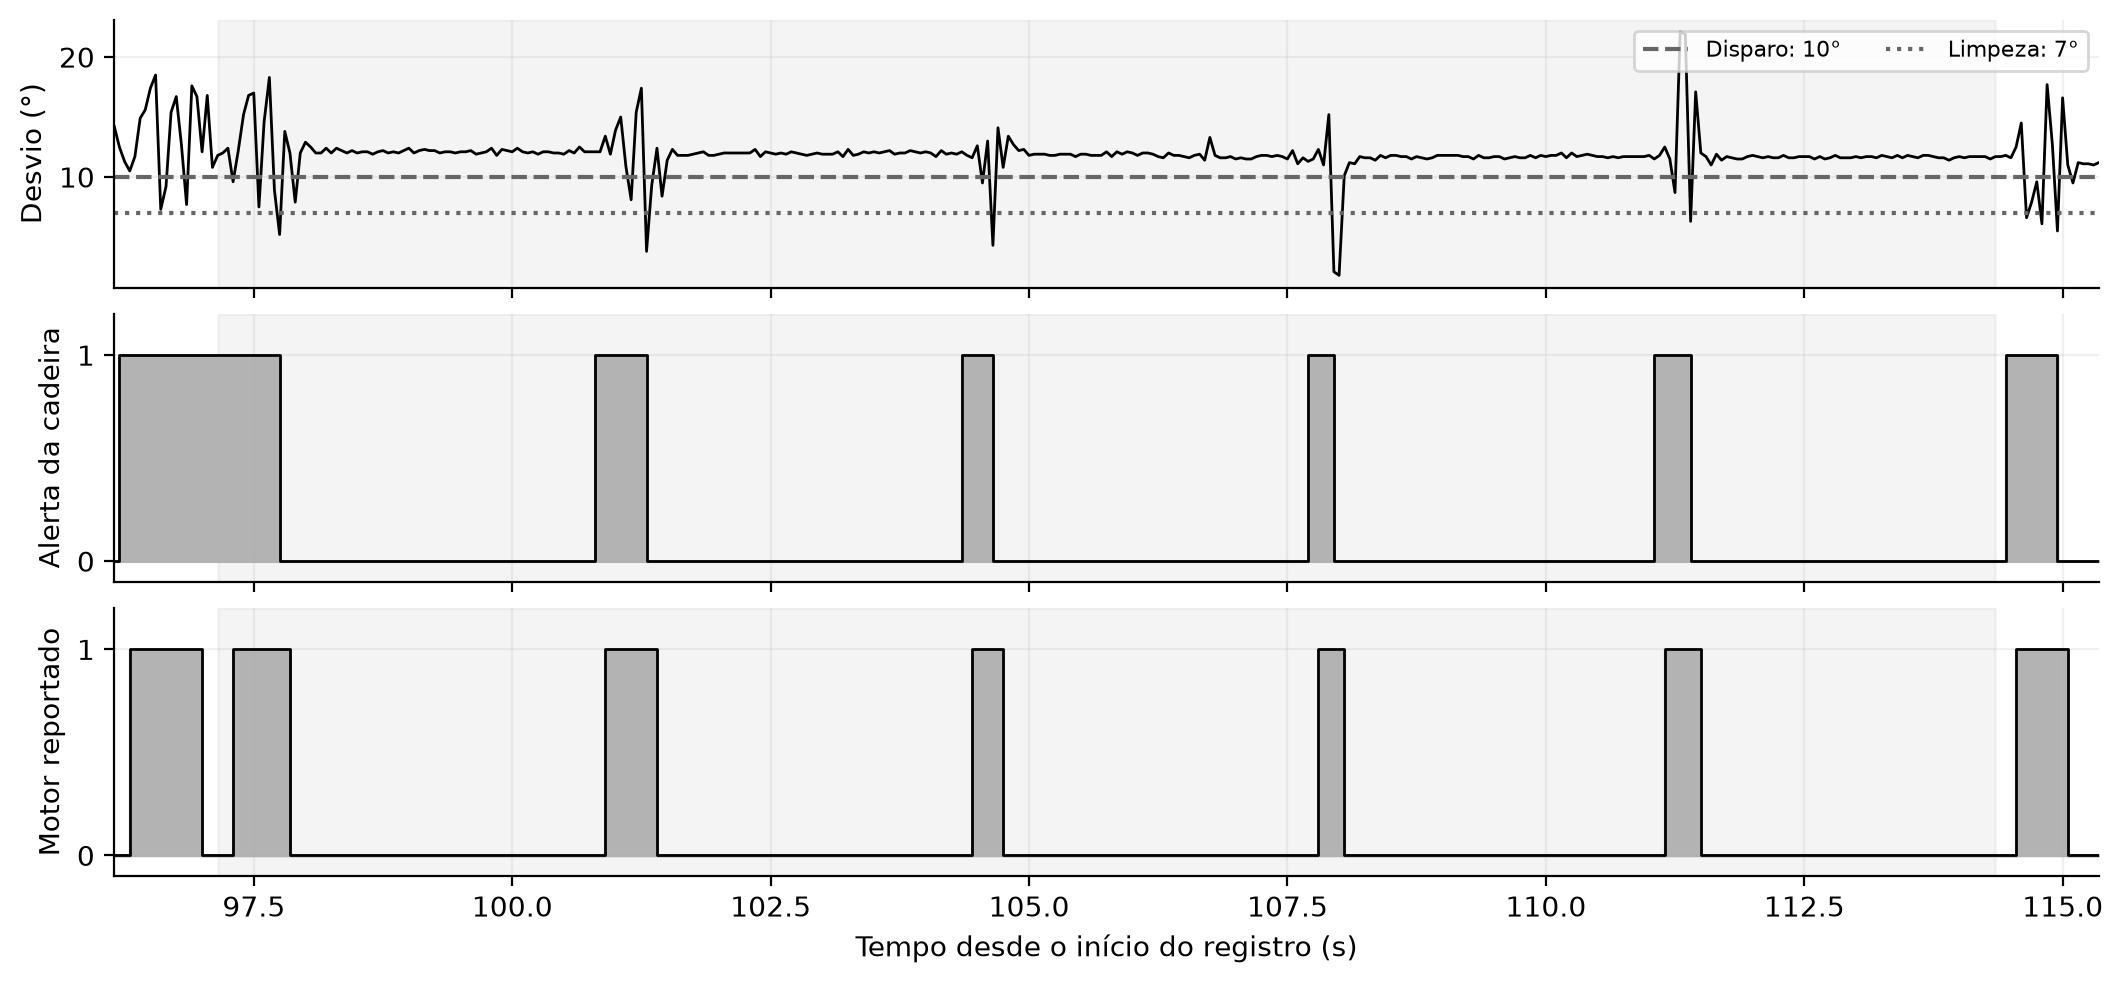
\includegraphics[width=\linewidth]{res_motor_lucas.png}
  \fonte{Elaborado pelo autor (2026)}
  \par\smallskip
  {\footnotesize O painel inferior apresenta o estado de motor reportado
  pelo corpo na coluna \texttt{bmotor}, e não uma medição elétrica do atuador.
  A faixa cinza corresponde ao segmento com etiqueta 5.}
\end{figure}

Considerando todo o segmento rotulado, o firmware alertou em
$11{,}6\,\%$ das amostras, valor arredondado para $12\,\%$ no registro
da sessão. Excluindo seus primeiros 2\,s, o valor foi $9{,}2\,\%$.
A reprodução atual fornece os mesmos $9{,}2\,\%$ nesse recorte; portanto,
a diferença entre ``12\,\% registrado'' e ``9\,\% reproduzido'' citada no
registro não se mantém ao igualar o denominador. Na postura 8, por outro
lado, o alerta registrado foi $2{,}9\,\%$ do tempo estabilizado, enquanto
a reprodução retornou $7{,}7\,\%$. Conserva-se o valor registrado na tabela
de hardware; a reprodução de ângulos arredondados em movimentos próximos aos
limiares não substitui o estado efetivamente executado nas placas.

A inclinação à direita de Lucas foi perdida: \texttt{dpitch} ficou próximo
de $+5{,}5\degree{}$, com redistribuição do assento para a esquerda,
contrária à condição de confirmação. O desvio lateral do segundo ereto
havia mudado aproximadamente $3{,}5\degree{}$ para a esquerda em relação
à referência inicial. Já a postura 8 produziu três alertas curtos associados
à condição lateral, com \texttt{dpitch} próximo de $-5{,}5\degree{}$, junto
à fronteira de $5\degree{}$. Os dois casos mostram que movimento do colar
e deslocamento causado pelas pernas podem aproximar posturas diferentes da
mesma fronteira de decisão.

\subsubsection{Correção posterior da interferência do atuador}

O histórico do firmware registra uma correção após essa validação, no
\textit{commit} \texttt{5e82e20}: enquanto o PWM do motor está ativo, o corpo
transmite a última leitura válida obtida com o motor desligado, evitando
substituí-la por uma leitura perturbada pela vibração. O limite dessa
retenção foi posteriormente ampliado para 1{,}5\,s no
\textit{commit} \texttt{6eaafbe}. A regra de fusão da cadeira permaneceu
inalterada.

A mensagem da correção relata uma reprodução com retenção dos ângulos em que
o alerta da inclinação à esquerda de Lucas passou de cerca de $9\,\%$ para
$100\,\%$, com mudança de aproximadamente $8\,\%$ para $11\,\%$ nas
pernas cruzadas e sem alteração no resultado de André. Esses números são
uma verificação por reprodução registrada no histórico, não uma nova sessão
física. Os dois arquivos de validação disponíveis foram obtidos com versões
anteriores à correção; não há nova captura registrada que confirme em hardware
o efeito da retenção. A demonstração posterior na feira, descrita a seguir,
fornece apenas evidência qualitativa e não supre essa comparação controlada.

\subsection{Demonstração na feira de ciências em novembro de 2026}
\label{sec:res-feira}

Na feira de ciências, dezenas de pessoas utilizaram cadeira instrumentada,
unidade corporal e alerta por vibração. Segundo o relato registrado no
projeto, a postura prejudicial foi detectada em praticamente todos os casos
observados. Houve nomes de postura divergentes do esperado em movimentos
combinados, mesmo com detecção da condição para alerta.

Sem arquivos das sessões, contagens de erros ou sequência padronizada,
não se calculam sensibilidade, especificidade ou taxa de acerto para a feira.
A evidência é qualitativa de funcionamento com várias pessoas fora da rodada
de desenvolvimento. Não se mediram mudança de hábito, redução de dor ou
benefício clínico.

\subsection{Enlace de comunicação e energia}
\label{sec:res-enlace-energia}

\subsubsection{Enlace ESB e monitoramento por beacon BLE}

No ensaio de bancada do enlace corpo--cadeira, a aproximadamente 1\,m, não
houve pacotes perdidos na taxa de 20\,Hz. Após a decisão ser transferida
para a cadeira e devolvida na carga útil de confirmação, foram observadas
aproximadamente 10--35 retransmissões por segundo. Portanto, ausência de
perda ao final das tentativas não significa ausência de repetição no rádio.
As sessões de validação de 22/10 também registraram zero perda de pacotes.
Esses resultados caracterizam os ensaios disponíveis, sem estabelecer alcance
máximo ou robustez sob outras condições de interferência.

O ensaio específico do \textit{beacon} BLE teve 60\,s de duração, com as
duas placas alimentadas por USB e recepção em um notebook com interface
MediaTek. Foram transmitidos 1200 anúncios e recebidos 225, correspondentes
a $3{,}75$ recepções por segundo e $18{,}75\,\%$ dos anúncios enviados.
A Tabela~\ref{tab:res-ble} sintetiza as lacunas. Os 225 registros recebidos
concordaram com os dados USB, com diferença de relógio de 0--1\,ms.
Nesse ensaio específico, o ESB manteve $20$ amostras por segundo, sem perda,
duplicação, pacotes inválidos, retransmissões ou entrada em modo de decisão
local por perda de enlace.

\begin{table}[H]
  \centering
  \caption{Recepção do beacon BLE no ensaio de bancada de 60 segundos.}
  \label{tab:res-ble}
  \begin{singlespace}
  \begin{tabularx}{\linewidth}{Xr}
    \toprule
    Indicador & Resultado \\
    \midrule
    Anúncios enviados / recebidos & 1200 / 225 \\
    Fração recebida & $18{,}75\,\%$ \\
    Taxa média de recepção & 3{,}75\,s$^{-1}$ \\
    Intensidade de sinal aproximada & $-73$\,dBm \\
    Mediana dos intervalos entre recepções & 175{,}5\,ms \\
    Percentil 90 dos intervalos & 500\,ms \\
    Maior intervalo & 1{,}9\,s \\
    \bottomrule
  \end{tabularx}
  \fonte{Elaborado pelo autor (2026)}
  \end{singlespace}
\end{table}

Os ensaios ESB com e sem retransmissões são observações distintas, sem
comparação controlada que explique a diferença ou encerre a questão.
O BLE permitiu exibir o estado recebido, mas suas lacunas impedem uma
captura completa. A decisão permanece autônoma pelo ESB; o notebook recebe
uma cópia. Os arquivos analisados neste capítulo foram obtidos por USB.

\subsubsection{Alimentação por bateria e medidas ainda ausentes}

O projeto registra funcionamento do corpo com LiPo e teste funcional
posterior da cadeira com o mesmo circuito. A célula corporal JYH LIP103450
é rotulada como 1800\,mAh e 3{,}7\,V; são especificações nominais, não
medidas de capacidade útil. O funcionamento sem USB não quantifica duração
da carga nem estabilidade do rádio durante a descarga.

No corpo, três leituras abaixo de 3{,}30\,V, sem USB e com motor desligado,
acionam \textit{System OFF}; a inicialização por bateria exige
3{,}40\,V. São limiares implementados, sem curva de descarga ou ensaio
completo registrado de corte e despertar por USB. O teste do beacon foi
alimentado por USB e não caracteriza seu consumo em bateria.

A pesquisa de alimentação registra correntes nominais de carga de $50$ ou
100\,mA e temporizador de segurança de aproximadamente dez horas.
Não se demonstrou carga completa em uma conexão ao USB, nem se mediram
tempo de recarga e energia reposta. Especificações de componentes não
fundamentam uma autonomia medida.

\pendente{Medir a corrente consumida por corpo e cadeira, discriminando
repouso operacional, comunicação e acionamento do motor, e registrando as
condições de alimentação e do beacon BLE.}

\pendente{Medir a autonomia de cada unidade por ciclo de descarga, com tensão
inicial, critério de término, padrão de alertas e condição do enlace
registrados; a capacidade nominal da bateria não substitui essa medição.}

% RASTREABILIDADE PARA INTEGRACAO (nao aparece no PDF):
% Bancada: report/relatorio_parcial.tex; analysis/archive/VALIDATION.md;
% analysis/archive/FSR_FINDINGS.md. As figuras antigas sao reaproveitadas.
% Conjunto: data/README.md; captures.py; execucao de report_figures.py.
% Fusao: docs/decisao-fusao-imu-fsr.md; execucao integral de fusion.py.
% Rafael tag 8: 24% com fusao (doc: celula '0/24' = atual/fusao).
% Lucas tag 5: log e replay = 11,594% integral, 9,180% estabilizado;
% registro compara 12% log a 9% replay sem igualar o denominador.
% Lucas tag 8: log estabilizado 2,950%, replay 7,670%; usa-se log em hardware.
% Correcao do motor: git show 5e82e20 e 6eaafbe; sem CSV posterior de validacao.
% Feira e bateria funcional das duas unidades: AGENTS.md (status nov/2026).
% ESB: AGENTS.md e TASKS.md; BLE: firmware/README.md.
% Energia: docs/pesquisa-bateria-lipo.md e firmware/README.md.
% Sem referencias bibliograficas novas; fontes internas de resultados proprios.

\section{Discussão}
\label{sec:discussao}

Este capítulo interpreta os resultados do Capítulo~\ref{sec:resultados} à luz
dos objetivos específicos, discute o papel de cada canal de sensoriamento na
decisão de alerta e consolida as limitações que restringem o alcance das
conclusões.

\subsection{Atendimento aos objetivos específicos}
\label{sec:dis-objetivos}

\paragraph{OE1 --- Variações anatômicas dos usuários.}
As variações entre pessoas apareceram em todos os níveis do sistema. Na
bancada, a simples retirada e recolocação do sensor deslocou a referência de
ereto em cerca de $8{,}0\degree{}$ (\textit{pitch}) e $21{,}6\degree{}$
(\textit{roll}), valores da mesma ordem do desvio que se deseja detectar. Nas
capturas integradas, a mesma instrução produziu amplitudes muito diferentes:
a inclinação à esquerda variou de $-6{,}2\degree{}$ (Felipe) a
$-27{,}1\degree{}$ (Rafael), e a cabeça à frente ficou entre $-4{,}6\degree{}$
e $-7{,}5\degree{}$ em três participantes, contra desvios bem maiores nos
demais. Na cadeira, alguns canais inferiores do encosto permaneceram próximos
de zero mesmo em ereto, conforme a estatura e o modo de sentar. A resposta de
projeto a essas variações foi dupla: a calibração individual da referência
angular (desvio, e não ângulo absoluto) e a normalização das leituras do
assento pela linha de base capturada na mesma janela. Com isso, a postura
ereta de cada pessoa passa a ser a origem do espaço de decisão, e o mesmo
limiar de $10\degree{}$ serviu a todos os participantes, com as exceções
discutidas na Seção~\ref{sec:dis-limitacoes}. O objetivo foi atendido no
sentido de \emph{caracterizar} as variações e \emph{acomodá-las} no projeto;
não se construiu um modelo antropométrico.

\paragraph{OE2 --- Sistema integrado com sensores.}
O sistema foi construído e operado como um todo: unidade vestível com IMU e
motor, cadeira com oito FSR402 multiplexados, enlace ESB a $20\,Hz$ com a
decisão devolvida na confirmação, alimentação por bateria nas duas unidades e
regra de fusão executada na cadeira. A regra embarcada é a mesma avaliada em
Python, verificada amostra a amostra pelo teste \texttt{test\_fusion}, o que
dá rastreabilidade entre análise e firmware. Nos ensaios de bancada e nas
sessões de validação não houve perda de pacotes no ESB. Em contrapartida, as
retransmissões aumentaram depois que a decisão passou a viajar no ACK, e o
consumo de energia não foi medido.

\paragraph{OE3 --- Comunicação com o usuário.}
O alerta háptico funcionou: na validação guiada, o participante percebeu a
vibração e sua interrupção ao voltar ao ereto, e o sistema foi operado por
dezenas de visitantes na feira. A validação com o primeiro sujeito novo
revelou, porém, uma interação não prevista entre atuador e sensor: a vibração
sacode o acelerômetro em cerca de $\pm10\degree{}$, uma amostra abaixo do
limiar de limpeza desligava o alerta e o portão de $3\,s$ recomeçava. Em vez
de um aviso sustentado, o usuário recebia pulsos esparsos. A correção
(retransmitir a última leitura obtida com o motor desligado) foi verificada
por reprodução dos dados, mas \emph{não} por uma nova sessão controlada em
hardware. Além da vibração, o LED de estado e o painel \texttt{mostra.py}
completam a comunicação; o painel, contudo, é um recurso de demonstração, e o
sistema permanece autônomo sem ele. O padrão de vibração atual (pulsos
de $700\,ms$ a cada segundo, sem pausa, enquanto durar o alerta) foi
considerado incômodo pelo autor durante os testes, o que remete ao problema de habituação e aceitação discutido na
literatura (Seção~\ref{sec:revisao}).

\paragraph{OE4 --- Eficiência do sistema.}
Tomando como critério a \emph{detecção} da postura prejudicial, a fusão,
avaliada deixando cada sujeito de fora (LOSO), alertou em 58 de 62 segmentos
prejudiciais e em $92\,\%$ do tempo prejudicial, com alerta em apenas $3\,\%$
do tempo em ereto ou reclinado. A regra só-IMU, que não foi ajustada a esses
dados, ficou em 55/62 segmentos, $84\,\%$ do tempo prejudicial e $29\,\%$ de
falso alarme em ereto/reclinado. A validação em hardware confirmou o
comportamento na rodada guiada ($100\,\%$ nas posturas 2--6 e $0\,\%$ nas
demais) e expôs, no sujeito novo, os três problemas descritos na
Seção~\ref{sec:res-hardware}. A feira acrescenta evidência qualitativa de
funcionamento com muitas pessoas. Esses números indicam viabilidade técnica
do detector; não medem a eficácia em mudar hábitos ou prevenir DORT, que
exigiria estudo longitudinal.

\subsection{O que cada canal acrescenta}
\label{sec:dis-fusao}

A hipótese que motivou o trabalho --- combinar a pressão na cadeira com a
orientação do tronco --- foi sustentada pelos dados, mas por um mecanismo
mais específico do que o previsto na entrega parcial. Ali, esperava-se que os
FSR separassem o par curvar-para-frente/cabeça-baixa, que o IMU confundia.
Nas capturas integradas, esse par não se mostrou o problema central para a
\emph{detecção}: ambas as posturas são prejudiciais, e o alerta não depende de
distingui-las. O ganho da fusão veio de três situações em que o ângulo do
tronco, sozinho, induz a decisão errada:
\begin{itemize}[nosep]
  \item \textbf{Reclinar com o quadril apoiado} produz desvio sagital semelhante
        ao de escorregar. Os FSR traseiros do assento mostram que o apoio foi
        mantido; o falso alarme no reclinado caiu de $78\,\%$ para $5\,\%$ do
        tempo. Na ablação, esse foi o maior incremento de pontuação.
  \item \textbf{Escorregar com pouca inclinação do tronco} passa despercebido
        pelo IMU, mas zera o assento traseiro; o escorregado passou de $72\,\%$
        para $100\,\%$ do tempo alertado.
  \item \textbf{Cadeira vazia}: com a pessoa em pé usando o colar, a regra
        só-IMU alertou em $71\,s$ de $176\,s$; a fusão, em nenhum instante.
\end{itemize}

A confirmação lateral pelo assento teve efeito menor e ambíguo: recuperou uma
inclinação pequena (Felipe), mas também gerou o falso alarme com pernas
cruzadas de Rafael e não confirmou a inclinação à direita de Vinicius e de
Lucas, em que a carga se deslocou no sentido oposto. Os resultados de bancada
anteciparam o modo correto de usar os FSR402: como indicadores de contato e
de pressão \emph{relativa}, comparados com a linha de base do próprio usuário,
e não como medidores de força. A regra final segue exatamente esse caminho
(somas de grupos do assento divididas pela linha de base), e a razão traseira
em ereto permaneceu entre $0{,}96$ e $1{,}09$ ao longo de sessões de até
$24$ minutos, longe dos limiares de $0{,}3$ e $0{,}7$, apesar do
\textit{creep} de $7$--$12\,\%$ medido em bancada.

\subsection{Detecção versus classificação}
\label{sec:dis-deteccao}

O sistema produz, junto com o alerta, um motivo (\texttt{SLUMP},
\texttt{IMU\_DEV}, \texttt{LEAN}) e o painel exibe um nome de postura. Os
erros de \emph{nome} observados na feira ocorreram em movimentos combinados ---
por exemplo, inclinar de lado e curvar ao mesmo tempo ---, situação para a
qual não há uma classe única correta. O mesmo fenômeno aparece nos dados
rotulados: Ryan permaneceu escorregado durante uma inclinação lateral e
Vinicius escorregou ao cruzar as pernas; nos dois casos o alerta foi
fisicamente justificado, embora a etiqueta não o previsse. Como a finalidade
do sistema é provocar a correção, e não diagnosticar a postura, avaliar pela
detecção é o critério adequado; a classificação é informação complementar
para o usuário e para a análise.

\subsection{Posicionamento em relação aos trabalhos relacionados}
\label{sec:dis-relacionados}

Os trabalhos com cadeiras instrumentadas resumidos na
Tabela~\ref{tab:rev-comparativo} buscam, em sua maioria, \emph{classificar}
posturas a partir de modelos treinados em outras pessoas, e relatam queda de
acerto quando o usuário não participou do treinamento --- de 96\,\% para
79\,\% em Tan, Slivovsky e Pentland (2001). Este trabalho segue caminho
diferente: em vez de um modelo geral, usa a postura ereta do próprio usuário
como referência e decide apenas se há desvio prejudicial. A avaliação LOSO
deste trabalho mede justamente a transferência a uma pessoa não usada no
ajuste dos parâmetros, e a perda observada (de $0{,}935$ para $0{,}901$ na
pontuação, com o mesmo número de segmentos prejudiciais detectados) foi
pequena. Os números, porém, não são comparáveis aos da tabela: as métricas,
as posturas e o tamanho das amostras diferem.

A revisão de Kappattanavar et al. (2021) não encontrou estudo que combinasse
pressão na cadeira com IMU vestível; o caso mais próximo, Zemp et al. (2016),
usa o módulo inercial no encosto, para medir a cadeira e não o usuário. Os
resultados da Seção~\ref{sec:dis-fusao} mostram por que a combinação importa:
os casos que mais pesaram na decisão --- reclinar apoiado e escorregar ---
são ambíguos para cada canal isolado e se resolvem quando os dois são
observados juntos. Em relação aos vestíveis com retorno vibratório, como o
avaliado por Kuo et al. (2021), a cadeira acrescenta contexto (presença,
apoio do quadril) que o sensor no corpo não tem; em relação ao BackWatch
(FERREIRA; SOUZA; CUBAS, 2025), que usa distância ao encosto com limiar fixo
e alerta visual, o sistema proposto acrescenta calibração individual,
orientação do tronco medida no corpo e alerta háptico. Por outro lado, a
literatura sobre biofeedback (Seção~\ref{sec:rev-feedback}) indica que o
efeito de curto prazo sobre a postura não garante benefício duradouro, o que
reforça que a eficácia clínica permanece fora do alcance deste trabalho.

\subsection{Limitações}
\label{sec:dis-limitacoes}

\begin{itemize}[nosep]
  \item \textbf{Amostra pequena e homogênea.} Oito participantes nas capturas e
        um único sujeito novo na validação em hardware. Não há estatística
        inferencial; os percentuais descrevem este conjunto.
  \item \textbf{Parâmetros ajustados nos mesmos dados.} A avaliação LOSO
        reduz, mas não elimina, o otimismo; a pontuação caiu de $0{,}935$ para
        $0{,}901$ e o falso alarme com pernas cruzadas subiu de $11\,\%$ para
        $28\,\%$ do tempo.
  \item \textbf{Posturas instruídas e mantidas.} As posturas foram executadas
        sob instrução, por cerca de $15\,s$, majoritariamente em ordem fixa e
        sem a série sutil prevista no protocolo. Não houve sessão de trabalho
        real prolongada.
  \item \textbf{Cabeça à frente.} Com o sensor no alto das costas, o movimento
        localizado do pescoço não foi detectado em três de sete participantes;
        os FSR não ajudam, pois as costas continuam apoiadas.
  \item \textbf{Fixação do colar.} A deriva da referência durante a sessão
        (Felipe, cerca de $+10\degree{}$; Lucas, cerca de $3{,}5\degree{}$)
        produziu falsos alarmes e perdas que nenhuma regra instantânea corrige.
  \item \textbf{Correção do motor não validada em hardware.} Os dois arquivos
        de validação são anteriores à retenção da leitura sem vibração.
  \item \textbf{Pernas cruzadas não tratadas.} Com quatro FSR no assento, o
        sinal não teve padrão comum entre pessoas; a regra deliberadamente não
        alerta nessa postura.
  \item \textbf{Uma cadeira, um colar.} Os limiares de contagem (vazio, linha
        de base mínima) dependem da espuma, da disposição dos sensores e do
        resistor do divisor desta cadeira.
  \item \textbf{Energia e latência não medidas.} Corrente, autonomia e o atraso
        entre o início físico da postura e a vibração não foram quantificados.
  \item \textbf{Feira sem registro.} O desempenho observado na feira é relato
        qualitativo e não entra nos números do trabalho.
\end{itemize}

\section{Conclusão}
\label{sec:conclusao}

Este trabalho investigou como um sistema inteligente pode monitorar a postura
de quem trabalha sentado e devolver, em tempo real, um aviso que leve à
autocorreção. Para isso, desenvolveu-se um protótipo completo e autônomo:
uma unidade vestível com IMU, posicionada logo abaixo do pescoço, e uma
cadeira de escritório com oito sensores de força resistivos, ligadas por um
enlace sem fio de baixa latência. A cadeira combina as duas fontes de
informação, decide quando a postura é prejudicial e envia o alerta, que a
unidade vestível converte em vibração.

Os resultados permitem três conclusões principais. Primeiro, a referência de
postura ereta varia entre pessoas e entre colocações do sensor em magnitude
comparável ao próprio desvio a detectar; por isso, a calibração individual
por botão, que define o ereto de cada usuário como origem, é condição para o
funcionamento, e não um refinamento. Segundo, sensores de força de baixo
custo, inadequados como medidores de força, mostraram-se suficientes como
indicadores de contato e de pressão relativa, desde que comparados com a
linha de base do próprio usuário. Terceiro, a fusão dessas leituras com a
orientação do tronco resolveu as falhas mais frequentes da abordagem baseada
apenas no IMU: deixou de alertar quando o usuário reclina com o quadril
apoiado ou se levanta da cadeira, e passou a detectar o escorregamento do
quadril mesmo com pouca inclinação do tronco. Nas capturas com oito
participantes, avaliadas deixando cada um de fora do ajuste, o sistema alertou
em 58 de 62 segmentos de postura prejudicial, com alerta em $3\,\%$ do tempo
em posturas aceitáveis; na demonstração pública, a postura prejudicial foi
detectada em praticamente todos os casos observados.

Esses resultados indicam a viabilidade técnica de detectar posturas
prejudiciais com a combinação proposta, mas não demonstram efeito sobre a
saúde. O conjunto de dados é pequeno, as posturas foram instruídas, e
permanecem limitações conhecidas: o movimento isolado da cabeça, a fixação do
colar ao longo da sessão, a interação entre vibração e sensor e o consumo de
energia.

\subsection{Trabalhos futuros}
\label{sec:trabalhos-futuros}

\begin{itemize}[nosep]
  \item \textbf{Validação ampliada:} novas sessões com mais participantes,
        posturas naturais e sutis, ordem embaralhada e uso prolongado em
        trabalho real, com o motor ativo e a correção da interferência do
        atuador já embarcada.
  \item \textbf{Padrão de vibração:} substituir os pulsos contínuos por um
        padrão com pausas crescentes, reduzindo incômodo e habituação, e
        avaliar a aceitação pelos usuários.
  \item \textbf{Energia:} medir corrente e autonomia de cada unidade; reduzir
        as retransmissões do enlace, desligar o rádio entre envios e baixar a
        taxa para $5$--$10\,Hz$, compatível com a dinâmica da postura.
  \item \textbf{Robustez da referência:} compensar a deriva lenta do colar
        quando o padrão dos FSR coincide com a linha de base, e aprimorar a
        fixação do invólucro.
  \item \textbf{Cabeça e pescoço:} investigar outra posição para o sensor ou
        um segundo IMU para detectar a projeção da cabeça à frente.
  \item \textbf{Assento:} avaliar mais pontos de pressão no assento para
        tratar pernas cruzadas e reduzir a dependência da espuma e do
        posicionamento de cada cadeira.
  \item \textbf{Efeito sobre o usuário:} estudo longitudinal que meça mudança
        de hábito postural e sintomas osteomusculares, por exemplo com o
        questionário nórdico, antes e depois do uso.
\end{itemize}


% =====================================================================
\clearpage
\section*{Referências}
\addcontentsline{toc}{section}{Referências}
\begin{singlespace}
\setlength{\parindent}{0pt}
\raggedright % ABNT NBR 6023: referências alinhadas à esquerda
\setlength{\parskip}{0.6em}

BOURAHMOUNE, K.; AMAGASA, T. AI-powered posture training: application of machine
learning in sitting posture recognition using the LifeChair smart cushion. In:
INTERNATIONAL JOINT CONFERENCE ON ARTIFICIAL INTELLIGENCE, 28., 2019, Macau.
\emph{Proceedings} [...]. [S.l.]: IJCAI, 2019. p. 5808--5814. DOI:
10.24963/ijcai.2019/805.

BREEN, P. P.; NISAR, A.; ÓLAIGHIN, G. Evaluation of a single accelerometer based
biofeedback system for real-time correction of neck posture in computer users.
In: ANNUAL INTERNATIONAL CONFERENCE OF THE IEEE ENGINEERING IN MEDICINE AND
BIOLOGY SOCIETY, 31., 2009, Minneapolis. \emph{Proceedings} [...]. Piscataway:
IEEE, 2009. p. 7269--7272. DOI: 10.1109/IEMBS.2009.5334726.

DUL, J.; WEERDMEESTER, B. \emph{Ergonomia prática}. 3. ed. São Paulo: Edgard
Blücher, 2012.

FERREIRA, J. A.; SOUZA, R. A. de; CUBAS, J. J. M. Desenvolvimento de um sistema
de monitoramento e alerta de postura utilizando sensores integrados em cadeira:
aplicação do BackWatch para melhoria da ergonomia. In: FEIRA BRASILEIRA DE
CIÊNCIAS E ENGENHARIA (FEBRACE), 2025, São Paulo. \emph{Mostra virtual}:
projeto SAU-8347. São Paulo: FEBRACE, 2025. Pôster. Disponível em: \url{https://virtual.febrace.org.br/2025/SAU/8347}. Acesso em: 8 nov. 2026.

GRANDJEAN, E. \emph{Manual de ergonomia}: adaptando o trabalho ao homem. 4. ed.
Porto Alegre: Bookman, 1998.

HALLER, M. et al. Finding the right way for interrupting people improving their
sitting posture. In: IFIP TC 13 INTERNATIONAL CONFERENCE ON HUMAN-COMPUTER
INTERACTION (INTERACT), 13., 2011, Lisboa. \emph{Human-Computer Interaction ---
INTERACT 2011}: part II. Berlin: Springer, 2011. p. 1--17. (Lecture Notes in
Computer Science, v. 6947). DOI: 10.1007/978-3-642-23771-3\_1.

IIDA, I.; GUIMARÃES, L. B. M. \emph{Ergonomia}: projeto e produção. 3. ed. São
Paulo: Edgard Blücher, 2016.

INTERLINK ELECTRONICS. \emph{FSR\textsuperscript{\textregistered} 400 Series data
sheet}. P/N PDS-10004-C. [S.l.]: Interlink Electronics, [2012?a]. Disponível em: \url{https://www.teachengineering.org/content/uconn_/activities/uconn-2662-contractions-calculations-force-resistance-activity/uconn-2662-contractions-calculations-FSR400series-datasheet.pdf}.
Acesso em: 8 nov. 2026.

INTERLINK ELECTRONICS. \emph{FSR\textsuperscript{\textregistered} integration
guide}. Doc. 94-00004 Rev. C. [S.l.]: Interlink Electronics, [2012?b].
Disponível em: \url{https://www.pololu.com/file/0J749/FSR400-Series-Integration-Guide-13.pdf}.
Acesso em: 8 nov. 2026.

INTERNATIONAL ORGANIZATION FOR STANDARDIZATION. \emph{ISO 11226}: ergonomics ---
evaluation of static working postures. Geneva: ISO, 2000.

KAPPATTANAVAR, A. M. et al. Monitoring of sitting postures with sensor networks in
controlled and free-living environments: systematic review. \emph{JMIR Biomedical
Engineering}, v. 6, n. 1, e21105, 2021. DOI: 10.2196/21105.

KUO, Y.-L. et al. Sitting posture during prolonged computer typing with and
without a wearable biofeedback sensor. \emph{International Journal of
Environmental Research and Public Health}, v. 18, n. 10, 5430, 2021. DOI:
10.3390/ijerph18105430.

KUORINKA, I. et al. Standardised Nordic questionnaires for the analysis of
musculoskeletal symptoms. \emph{Applied Ergonomics}, v. 18, n. 3, p. 233--237,
1987.

LUINGE, H. J.; VELTINK, P. H. Measuring orientation of human body segments using
miniature gyroscopes and accelerometers. \emph{Medical and Biological Engineering
and Computing}, v. 43, p. 273--282, 2005. DOI: 10.1007/BF02345966.

MCATAMNEY, L.; CORLETT, E. N. RULA: a survey method for the investigation of
work-related upper limb disorders. \emph{Applied Ergonomics}, v. 24, n. 2,
p. 91--99, 1993.

MEYER, J. et al. Design and modeling of a textile pressure sensor for sitting
posture classification. \emph{IEEE Sensors Journal}, v. 10, n. 8,
p. 1391--1398, 2010. DOI: 10.1109/JSEN.2009.2037330.

MOHAMMADIAN et al. Musculoskeletal disorders among office workers: prevalence,
ergonomic risk factors, and their interrelationships. \emph{Scientific Reports},
v. 15, 2025. DOI: 10.1038/s41598-025-30155-6.

MUTLU, B. et al. Robust, low-cost, non-intrusive sensing and recognition of
seated postures. In: ANNUAL ACM SYMPOSIUM ON USER INTERFACE SOFTWARE AND
TECHNOLOGY, 20., 2007, Newport. \emph{Proceedings} [...]. New York: ACM, 2007.
p. 149--158. DOI: 10.1145/1294211.1294237.

OKEZUE, O. C. et al. Work-Related Musculoskeletal Disorders among Office Workers
in Higher Education Institutions: A Cross-Sectional Study. \emph{Ethiopian
Journal of Health Sciences}, v. 30, n. 5, p. 715--724, 2020.

PAREDES-MADRID, L. et al. Underlying physics of conductive polymer composites and
force sensing resistors (FSRs): a study on creep response and dynamic loading.
\emph{Materials}, v. 10, n. 11, 1334, 2017. DOI: 10.3390/ma10111334.

PEDLEY, M. \emph{Tilt sensing using a three-axis accelerometer}. Application
Note AN3461, Rev. 6. [S.l.]: Freescale Semiconductor, 2013. Disponível em: \url{https://www.nxp.jp/docs/en/application-note/AN3461.pdf}. Acesso em: 8 nov. 2026.

RIBEIRO, D. C.; SOLE, G.; ABBOTT, J. H.; MILOSAVLJEVIC, S. The effectiveness of a
lumbopelvic monitor and feedback device to change postural behavior: a
feasibility randomized controlled trial. \emph{Journal of Orthopaedic \& Sports
Physical Therapy}, v. 44, n. 9, p. 702--711, 2014. DOI: 10.2519/jospt.2014.5009.

RIBEIRO, D. C. et al. Effectiveness of a lumbopelvic monitor and feedback device
to change postural behaviour: the ELF cluster randomised controlled trial.
\emph{Occupational and Environmental Medicine}, v. 77, n. 7, p. 462--469, 2020.
DOI: 10.1136/oemed-2019-106293.

ROBERTSON, M.; CIRIELLO, V.; GARABET, A. Office ergonomics training and a
sit-stand workstation: effects on musculoskeletal and visual symptoms and
performance of office workers. \emph{Applied Ergonomics}, v. 44, n. 1,
p. 73--85, 2013.

ROH, J. et al. Sitting posture monitoring system based on a low-cost load cell
using machine learning. \emph{Sensors}, v. 18, n. 1, 208, 2018. DOI:
10.3390/s18010208.

SONNE, M.; VILLALTA, D. L.; ANDREWS, D. M. Development and evaluation of an
office ergonomic risk checklist: ROSA --- Rapid Office Strain Assessment.
\emph{Applied Ergonomics}, v. 43, n. 1, p. 98--108, 2012.

TAN, H. Z.; SLIVOVSKY, L. A.; PENTLAND, A. A sensing chair using pressure
distribution sensors. \emph{IEEE/ASME Transactions on Mechatronics}, v. 6, n. 3,
p. 261--268, 2001. DOI: 10.1109/3516.951364.

WONG, W. Y.; WONG, M. S. Trunk posture monitoring with inertial sensors.
\emph{European Spine Journal}, v. 17, n. 5, p. 743--753, 2008. DOI:
10.1007/s00586-008-0586-0.

XU, W. et al. eCushion: a textile pressure sensor array design and calibration
for sitting posture analysis. \emph{IEEE Sensors Journal}, v. 13, n. 10,
p. 3926--3934, 2013. DOI: 10.1109/JSEN.2013.2259589.

ZEMP, R. et al. Application of machine learning approaches for classifying
sitting posture based on force and acceleration sensors. \emph{BioMed Research
International}, v. 2016, 5978489, 2016. DOI: 10.1155/2016/5978489.

ZHENG, Y.; MORRELL, J. B. Comparison of visual and vibrotactile feedback methods
for seated posture guidance. \emph{IEEE Transactions on Haptics}, v. 6, n. 1,
p. 13--23, 2013. DOI: 10.1109/TOH.2012.3.
\end{singlespace}


\end{document}
